%stylefile for "Progress in Particle and Nuclear Physics" from 20. March 2003
\documentclass[twoside,12pt]{article}
\usepackage{epsfig}
%\usepackage{amssymb}
\usepackage{amsmath, amssymb}

%%%%%%% TEMPORARY %%%%%%%%%
\usepackage{color}
%\usepackage{hyperref}% add hypertext capabilities

\definecolor{gray}{rgb}{0.5,0.5,0.5}
\newcommand{\com}[1]{{\color{red} \sffamily (#1)}}
\newcommand{\omi}[1]{{\color{gray}\tiny\bfseries [#1]}}
\newcommand{\add}[1]{{\bfseries #1}}
%%%%%%%%%%%%%%%%%%%%%%%

\def\Journal#1#2#3#4{{#1} {#2} (#4) #3 }
\def\NCA{{\em Nuovo Cimento} A}
\def\PHYS{{\em Physica}}
\def\NPA{{\em Nucl. Phys.} A}
\def\MATH{{\em J. Math. Phys.}}
\def\PRO{{\em Prog. Theor. Phys.}}
\def\NPB{{\em Nucl. Phys.} B}
\def\PLA{{\em Phys. Lett.} A}
\def\PLB{{\em Phys. Lett.} B}
\def\PLD{{\em Phys. Lett.} D}
\def\PL{{\em Phys. Lett.}}
\def\PRL{\em Phys. Rev. Lett.}
\def\PREV{\em Phys. Rev.}
\def\PREP{\em Phys. Rep.}
\def\PRA{{\em Phys. Rev.} A}
\def\PRD{{\em Phys. Rev.} D}
\def\PRC{{\em Phys. Rev.} C}
\def\PRB{{\em Phys. Rev.} B}
\def\ZPC{{\em Z. Phys.} C}
\def\ZPA{{\em Z. Phys.} A}
\def\ANNP{\em Ann. Phys. (N.Y.)}
\def\RMP{{\em Rev. Mod. Phys.}}
\def\CHEM{{\em J. Chem. Phys.}}
\def\INT{{\em Int. J. Mod. Phys.} E}
\def\r{\vec r}
\def\R{\vec R}
\def\p{\vec p}
\def\P{\vec P}
\def\q{\vec q}
\def\ss{\mbox{\boldmath $\sigma$}}
\newcommand{\be}{\begin{equation}}
\newcommand{\eeq}{\end{equation}}
\newcommand{\bea}{\begin{eqnarray}}
\newcommand{\eea}{\end{eqnarray}}
\newcommand{\nn}{\nonumber}
\topmargin-2.8cm
\oddsidemargin-1cm
\evensidemargin-1cm
\textwidth18.5cm
\textheight25.0cm


\input symbols


%%% ??????
%\bibliographystyle{elsarticle-harv} 
\bibliographystyle{ieeetr}

\begin{document}

%\begin{frontmatter}

%% Title, authors and addresses

%% use the tnoteref command within \title for footnotes;
%% use the tnotetext command for theassociated footnote;
%% use the fnref command within \author or \address for footnotes;
%% use the fntext command for theassociated footnote;
%% use the corref command within \author for corresponding author footnotes;
%% use the cortext command for theassociated footnote;
%% use the ead command for the email address,
%% and the form \ead[url] for the home page:
%% \title{Title\tnoteref{label1}}
%% \tnotetext[label1]{}
%% \author{Name\corref{cor1}\fnref{label2}}
%% \ead{email address}
%% \ead[url]{home page}
%% \fntext[label2]{}
%% \cortext[cor1]{}
%% \address{Address\fnref{label3}}
%% \fntext[label3]{}

\title{Neutrino oscillations: the rise of the PMNS paradigm}

%% use optional labels to link authors explicitly to addresses:
%% \author[label1,label2]{}
%% \address[label1]{}
%% \address[label2]{}
\author{C. Giganti$^1$, S.\ Lavignac$^2$, M.\ Zito$^3$ \\
\\
$^1$ LPNHE, CNRS/IN2P3, UPMC, Universit\'{e} Paris Diderot, Paris 75252, France\\
$^2$Institut de Physique Th\'{e}orique,
Universit\'e Paris Saclay, CNRS, CEA,\\
Gif-sur-Yvette, France\footnote{Unit\'e Mixte de Recherche
du CEA/DRF et du CNRS (UMR 3681).}\\
$^3$IRFU/SPP, CEA-Saclay, Gif-sur-Yvette, France}

\maketitle
\begin{abstract}
%% Text of abstract

In the last two decades neutrino physics has undergone a tremendous progress following the discovery of neutrino oscillations. 
Since this milestone, experimental progress has been very fast with the first indications in 2011 by T2K of the last unknown mixing angle $\theta_{13}$, the discovery of $\nu_\mu \rightarrow \nu_e$ appearance by that same experiment,  and the discovery and precision measurement of $\theta_{13}$ by the reactor experiments Daya Bay, RENO and Double Chooz. 

Today a very large set of experimental results obtained with a variety of experimental configurations and techniques can be interpreted in the framework of three active massive neutrinos, whose mass and flavour eigenstates are related by  the Pontecorvo-Maki-Nakagawa-Sakata (PMNS) 3 $\times$ 3 unitary mixing matrix parameterized by the mixing angles $\theta_{12}$,$\theta_{23}$ and $\theta_{13}$, and the CP-violation phase \dcp. Additional parameters governing the neutrino oscillations are the squared mass differences $\Delta m^2_{ij}=m^2_j-m^2_i$  between the three neutrino mass eigenstates with eigenvalues $m_1$, $m_2$, and $m_3$. This review covers the rise of this PMNS three neutrinos mixing paradigm and the current status of the experimental determination of its parameters.

The next years will continue to see a rich program of experimental endeavour coming to fruition and addressing the three last missing pieces of the puzzle, namely the precision determination of the $\theta_{23}$ value and octant, the unveiling of the neutrino mass ordering (whether $m_1 < m_2 < m_3$ or $m_3 < m_1 < m_2$) and the measurement of the CP-violating phase \dcp.


\end{abstract}

%\begin{keyword}
%% keywords here, in the form: keyword \sep keyword

%% PACS codes here, in the form: \PACS code \sep code

%% MSC codes here, in the form: \MSC code \sep code
%% or \MSC[2008] code \sep code (2000 is the default)

%\end{keyword}

%\end{frontmatter}

%% \linenumbers

%% main text

\tableofcontents
%% Introduction
\section{Introduction}
\label{sec:intro}

In the last two decades neutrino physics has undergone a tremendous progress related to the discovery of neutrino oscillations. It is remarkable that after a very long period of theoretical and experimental work, sometimes marked by heated controversies and debates, the original intuition by Bruno Pontecorvo in 1957 \cite{pontecorvo1, pontecorvo2} was at last confirmed in the few years between 1996 and 2003 by the beautiful discoveries of the neutrino oscillations in the atmospheric and in the solar sectors. These discoveries have been properly recognized with the 2015 Nobel Prize in Physics to Takaaki Kajita and Arthur Mc Donald.

Since this milestone, experimental progress has been very fast with the first indications by T2K\cite{t2k2011} of the last mixing angle $\theta_{13}$ and then its discovery by the reactor experiments Double Chooz, RENO and Daya Bay. While experiments with natural sources have been at the forefront of the discovery of neutrino oscillations, recent precision measurements have been mainly been carried out with man-made sources, like nuclear reactors and neutrino beams. 

Today a very large set of experimental results obtained with an amazing variety of experimental configurations and techniques can be interpreted in the framework of the Pontecorvo-Maki-Nakagawa-Sakata (PMNS) framework, consisting of a 3 $\times$ 3 unitary mixing matrix and the mass squared differences of the mass eigenstates. This review covers mainly the rise of this PMNS three neutrinos mixing paradigm and the current status of the experimental determination of its parameters.

As we will discuss later, the next years will continue to see a rich program of experimental endeavour coming to fruition and addressing the three last missing pieces of the puzzle, namely the precision determination of the $\theta_{23}$ value and octant, the unveiling of the neutrino mass ordering and the measurement of the CP-violating phase $\delta$.

The study of neutrinos, and of neutrino oscillations in particular, plays a special role in our understanding of particle physics and at the frontier of our knowledges in this domain. Indeed, the measurement of the neutrino mass as different from zero, whose only experimental evidence comes from neutrino oscillations, is our first positive indication of physics beyond the Standard Model (add reference). Moreover, the global picture of the neutrino mixing matrix is radically different from the analogous CKM mixing matrix in the quark sector and this in itself represents a deep question that needs to be addressed and understood.

Interestingly, the large mixing angles of the PMNS matrix open the possibility for significant CP violation in the lepton sector. These studies might help our understanding of the baryon asymmetry in the universe, whose best interpretive framework is today represented by the leptogenesis model.
 
This review is organized as follows. We first introduce the massive neutrino mixing formalism, with particular emphasis on a pedagogical approach for students and scholars entering this field. Then we discuss the experimental evidence for neutrino oscillations in the three historical sectors, namely the study of solar neutrinos and $\theta_{12}$ angle, then the atmospheric neutrinos and the $\theta_{23}$ angle and finally the last discovered sector parametrized by the $\theta_{13}$ angle. In each of these sectors, the relation between experimental results and theory can be easily understood on the basis of effective two neutrino mixing formulae, even though the experimental precision increasingly requires to take into account higher order effects. We then turn to the new phenomena that can only be interpreted as genuine three neutrino effects, and especially the study of CP violation effects that has been initiated by the T2K and NOvA experiments. To conclude this section, we briefly summarize our current level of understanding of the various parameters of the PMNS framework and the role played by global fits.

After briefly mentioning the remaining anomalies that can not be interpreted inside the PMNS framework, we turn to the presenting an overview of the future experimental program and how it can answer the remaining questions. 


%% Theoretical description
\section{Theory and phenomenology of oscillations 15 pg SL}
\label{sec:th}


Neutrino oscillations are a quantum-mechanical phenomenon that is made possible
by the existence of non-degenerate neutrino masses and lepton flavour mixing.
As for quarks, the origin of flavour mixing in the lepton sector is the mismatch between
the basis of (weak) gauge eigenstates %(also called {\it flavour eigenstates})
and the basis of mass eigenstates,
namely the fact that the neutrino mass matrix is not diagonal when written in the flavour basis
(i.e. the weak eigenstate basis corresponding to the charged lepton mass eigenstates
$e$, $\mu$ and $\tau$).
%the neutrino to which a given charged lepton (electron, muon or tau) couples
%via the charged current is not a mass eigenstate, but a coherent superposition
%of mass eigenstates.
The relative rotation between the flavour and the mass eigenstate left-handed neutrino fields
is the {\it lepton mixing matrix}, known as the PMNS (Pontecorvo-Maki-Nakagawa-Sakata) matrix:
%
\be
  \left(\!\! \begin{array}{c} \nu_e(x) \\ \nu_\mu(x) \\ \nu_\tau(x) \end{array}\!\! \right)_{\!\!L}
  =\, U\, \left(\!\! \begin{array}{c} \nu_1(x) \\ \nu_2(x) \\ \nu_3(x) \end{array}\!\! \right)_{\!\!L}
  =\, \left(\! \begin{array}{ccc} U_{e1} & U_{e2} & U_{e3} \\ U_{\mu1} & U_{\mu2} & U_{\mu3} \\ U_{\tau 1}
    & U_{\tau2} & U_{\tau3} \end{array}\! \right)\! \left(\!\!
    \begin{array}{c} \nu_1(x) \\ \nu_2(x) \\ \nu_3(x) \end{array}\!\! \right)_{\!\!L}\, .
\label{eq:flavour_mass_relation_long}
\eeq
%
In Eq.~(\ref{eq:flavour_mass_relation_long}),
$\nu_{e L} (x)$, $\nu_{\mu L} (x)$ and $\nu_{\tau L} (x)$ are the fields describing
the left-handed {\it flavour eigenstate} neutrinos,
defined as the neutrinos that couple via charged weak current to the electron, the muon
and the tau, respectively,
and $\nu_{1 L} (x)$, $\nu_{2 L} (x)$ and $\nu_{3 L} (x)$ describe the left-handed
mass eigenstate neutrinos with masses $m_1$, $m_2$ and $m_3$.
%%
%\be
%  \left(\! \begin{array}{c} \nu_e(x) \\ \nu_\mu(x) \\ \nu_\tau(x) \end{array}\! \right)_{\!\!L}
%  =\, U_{\rm PMNS} \left(\! \begin{array}{c} \nu_1(x) \\ \nu_2(x) \\ \nu_3(x) \end{array}\! \right)_{\!\!L}
%  =\, \left(\! \begin{array}{ccc} U_{e1} & U_{e2} & U_{e3} \\ U_{\mu1} & U_{\mu2} & U_{\mu3} \\ U_{\tau 1}
%    & U_{\tau2} & U_{\tau3} \end{array}\! \right)\! \left(\!
%    \begin{array}{c} \nu_1(x) \\ \nu_2(x) \\ \nu_3(x) \end{array}\! \right)_{\!\!L}\, .
%\eeq
%%
In shorthand notations, the relation~(\ref{eq:flavour_mass_relation_long}) reduces to
%between the flavour and mass eigenstate neutrino fields
%
\be
  \nu_{\alpha L} (x)\, =\, \sum_i U_{\alpha i} \nu_{i L} (x)\, ,
\label{eq:flavour_mass_relation}
\eeq
%
where $\alpha = e, \mu, \tau$ and $i=1,2,3$.
In the following, we shall omit the subscript ``$L$'' for simplicity.
As a consequence of flavour mixing,
the neutrino that couples to a charged lepton of a given flavour (an electron,
a muon or a tau) is not a mass eigenstate, but a {\it coherent superposition of mass eigenstates}:
%%
%\be
%  {\cal L}_{\rm CC}\, =\, \frac{g}{\sqrt{2}}\ W^-_\mu \sum_\alpha\, \bar e_{\alpha L} \gamma^\mu \nu_{\alpha L}\,
%    =\, \frac{g}{\sqrt{2}}\ W^-_\mu \sum_{\alpha, i}\, U_{\alpha i}\, \bar e_{\alpha L} \gamma^\mu \nu_{i L}\, .
%\ee
%%
%
\be
  {\cal L}_{\rm CC}\, =\, \frac{g}{\sqrt{2}}\ W^-_\mu
    \sum_{\alpha = e, \mu, \tau}\! \bar e_{\alpha L} \gamma^\mu \nu_{\alpha L}\,
  =\, \frac{g}{\sqrt{2}}\ W^-_\mu \sum_{\alpha = e, \mu, \tau}\! \bar e_{\alpha L} \gamma^\mu
    \sum_{i = 1,2,3}\! U_{\alpha i}\, \nu_{i L}\, .
\label{eq:L_CC}
\eeq
%
%%
%\be
%  {\cal L}_{\rm CC}\, =\, \frac{g}{\sqrt{2}}\ W^-_\mu\!
%    \sum_{\alpha = e, \mu, \tau}\! \bar e_{\alpha L} \gamma^\mu \nu_{\alpha L}\,
%  =\, \frac{g}{\sqrt{2}}\ W^-_\mu\! \sum_{\alpha = e, \mu, \tau}\! \bar e_{\alpha L} \gamma^\mu\,
%    \sum_i\, U_{\alpha i} \nu_{i L}\, .
%\label{eq:L_CC}
%\eeq
%%
%%
%\be
%  {\cal L}_{\rm CC}\, =\, \frac{g}{\sqrt{2}}\ W^-_\mu \sum_\alpha\, \bar e_{\alpha L} \gamma^\mu \nu_{\alpha L}\,
%    =\, \frac{g}{\sqrt{2}}\ W^-_\mu \sum_\alpha\, \bar e_{\alpha L} \gamma^\mu \sum_i\, U_{\alpha i} \nu_{i L}\, .
%\eeq
%%
It is this coherence that makes neutrino oscillations possible.
%\omi{Neutral current, on the contrary,
%is not sensitive to flavour mixing, since $\sum_\alpha \bar \nu_{\alpha L} \gamma^\mu \nu_{\alpha L}
%= \sum_{i,j} \sum_\alpha U^*_{\alpha j} U_{\alpha i}\, \bar \nu_{j L} \gamma^\mu \nu_{i L}
%= \sum_{i,j} \delta_{i j}\, \bar \nu_{j L} \gamma^\mu \nu_{i L} = \sum_i \bar \nu_{i L} \gamma^\mu \nu_{i L}$.}

Being associated with a change of basis, the PMNS matrix is a unitary matrix. Like the CKM matrix,
it satisfies unitary relations, derived from $U U^\dagger = U^\dagger U = \mathbf{1}$:
%
\be
  \sum_i\, U_{\alpha i} U^*_{\beta i}\, =\, \delta_{\alpha \beta} \quad \left( \alpha, \beta = e, \mu, \tau \right) ,
  \qquad  \sum_\alpha\, U^*_{\alpha i} U_{\alpha j}\, =\, \delta_{ij} \quad \left( i, j = 1,2,3 \right) .
\eeq
%
Like any $3 \times 3$ unitary matrix, $U$ can be parametrized by 3 mixing angles and 6 phases.
However, not all of these phases are physical, since lepton fields can be rephased
to absorb some of them. Namely, if neutrinos are Dirac fermions, one can rephase
both the charged lepton and the neutrino fields, $e_\alpha (x) \to e^{i\phi_\alpha}\, e_\alpha (x)$
and $\nu_i (x) \to e^{i\phi_i}\, \nu_i (x)$, where $e_\alpha (x)$ and $\nu_i (x)$ denote
the 4-component Dirac fields (i.e. the phases of the left-handed and right-handed lepton fields
are shifted by the same amount, in order not to affect the mass terms
$- \sum_\alpha m_{\ell_\alpha} \bar e_{R \alpha} e_{L \alpha} - \sum_i m_i  \bar \nu_{R i} \nu_{L i} + \mbox{h.c.}$).
%This leaves the Lagrangian invariant, including the charged current
%term~(\ref{eq:L_CC}), provided that the PMNS matrix is redefined in the following way:
This leaves the charged current term~(\ref{eq:L_CC}) invariant, provided that one redefines
the PMNS matrix in the following way:
%
\be
  U_{\alpha i}\, \to\, e^{i (\phi_\alpha - \phi_i)}\, U_{\alpha i}\, .
\eeq
%
Since there are 5 independent phase differences $\phi_\alpha - \phi_i$, one can
remove 5 phases from the PMNS matrix, leaving only one physical CP-violating
phase, as in the CKM matrix. If neutrinos are Majorana fermions, however, it is
not possible to rephase the left-handed neutrino fields, because this would make
their masses complex (indeed, Majorana mass terms are of the form
$- \frac{1}{2}\, m_i\, \nu^T_{L i} C \nu_{L i} + \mbox{h.c.}$, where $C$ is the charge
conjugation matrix satisfying $C \gamma_\mu C^{-1} = - \gamma^T_\mu$).
%Thus only the charged lepton fields can be rephased and only 3 phases can be removed
%from the PMNS matrix (as $U_{\alpha i}\, \to\, e^{i \phi_\alpha}\, U_{\alpha i}$),
%leaving 3 physical CP-violating phases.
Thus only the charged lepton fields can be rephased, leading to
%
\be
  U_{\alpha i}\, \to\, e^{i \phi_\alpha}\, U_{\alpha i}\, .
\eeq
%
One is therefore left with 3 physical CP-violating phases in the Majorana case,
instead of a single one in the Dirac case\footnote{This parameter counting can be
generalized to an arbitrary number $N$ of lepton flavours,
%but this exercise is of rather academic interest, given that the number of active neutrinos
%is known to be 3 without ambiguity (sterile neutrinos may however exist, but the counting
although the number of active neutrinos
is known to be 3 without ambiguity (sterile neutrinos may exist, but the counting
of physical mixing parameters is different in this case, see Section~\ref{subsec:steriles}).
One finds, in the Dirac case, $N(N-1)/2$ mixing angles
and $(N-1)(N-2)/2$ phases, and $N-1$ additional phases in the Majorana case.
Thus, at variance with the quark sector, CP violation is possible already with 2 generations
of leptons if neutrinos are Majorana fermions. Nevertheless, for reasons that will become clear below,
CP violation in oscillations requires at least 3 generations.}.


%The standard parametrization of the PMNS matrix is
%The PMNS matrix can therefore be written as the product of three rotations
Based on this parameter counting, the PMNS matrix can be written as the product of three rotations
through angles $\theta_{23}$, $\theta_{13}$ and $\theta_{12}$,  where the second
(unitary) rotation depends on a phase $\delta$, and of a diagonal matrix of phases $P$:
%
\bea
  U\! & =\! & \left( \begin{array}{ccc} 1 & 0 & 0 \\ 0 & c_{23} & s_{23} \\ 0 & - s_{23} & c_{23} \end{array} \right)
    \left( \begin{array}{ccc} c_{13} & 0 & s_{13} e^{-i \delta} \\ 0 & 1 & 0 \\ - s_{13} e^{i \delta} & 0 & c_{13} \end{array} \right)
    \left( \begin{array}{ccc} c_{12} & s_{12} & 0 \\ - s_{12} & c_{12} & 0 \\ 0 & 0 & 1 \end{array} \right) P  \nn \\
  & =\! & \left( \begin{array}{ccc} c_{12} c_{13} & s_{12} c_{13} & s_{13} e^{-i \delta} \\
    - s_{12} c_{23} - c_{12} s_{13} s_{23} e^{i \delta} & c_{12} c_{23} - s_{12} s_{13} s_{23} e^{i \delta} & c_{13} s_{23} \\
    s_{12} s_{23} - c_{12} s_{13} c_{23} e^{i \delta} & - c_{12} s_{23} - s_{12} s_{13} c_{23} e^{i \delta} & c_{13} c_{23} 
   \end{array} \right) P\ .
\label{eq:PMNS}
\eea
%
In Eq.~(\ref{eq:PMNS}), $c_{ij} \equiv \cos \theta_{ij}$, $s_{ij} \equiv \sin \theta_{ij}$ and $P$
is either the unit matrix $\mathbf{1}$ in the Dirac case, or a diagonal matrix containing
the two phases associated with the Majorana nature of neutrinos in the Majorana case.
Without loss of generality, one can take $\theta_{ij} \in \left[ 0, \frac{\pi}{2} \right]$ and
$\delta \in \left[ 0, 2 \pi \right[$.
%Except for the explicit form of $P$ in the Majorana case, this parametrization has now become
%standard. The following conventions for the Majorana phases can be found in the literature:
This parametrization has now become standard, except for the explicit form of the matrix $P$
in the Majorana case, for which different conventions can be found in the literature, e.g.
%
\be
  P_{\rm Majorana}\, =\, \left( \begin{array}{ccc} e^{i \alpha_1} & 0 & 0 \\ 0 & e^{i \alpha_2} & 0 \\ 0 & 0 & 1 \end{array} \right) ,
    \quad %\mbox{or} \quad
  \left( \begin{array}{ccc} 1 & 0 & 0 \\ 0 & e^{i \phi_2} & 0 \\ 0 & 0 & e^{i \phi_3} \end{array} \right) ,
    \quad %\mbox{or} \quad
  \left( \begin{array}{ccc} e^{i \rho} & 0 & 0 \\ 0 & 1 & 0 \\ 0 & 0 & e^{i \sigma} \end{array} \right) .
    %\quad \mbox{or \dots}  \hskip .3cm
\eeq
%
All these choices are related by rephasings of the charged lepton fields and are
therefore physically equivalent.
%All these conventions are physically equivalent, since one can change from one to another
%by an overall rephasing of the charged lepton fields, $e_\alpha (x) \to e^{i\phi}\, e_\alpha (x)$.
The phase $\delta$ is often called the ``Dirac phase'' of the PMNS matrix, while
the phases contained in $P$, which can be restricted to the range $\left[ 0, \pi \right[$
without loss of generality, are dubbed ``Majorana phases''. 
We will not be concerned with Majorana phases in this review because, as we are
going to see, they do not enter oscillation probabilities.
They appear only in lepton number violating processes like neutrinoless double beta decay,
in which the Majorana nature of neutrinos plays a crucial role.
The phase $\delta$, on the contrary, is relevant to neutrino oscillations and gives
rise to an asymmetry between neutrino and antineutrino oscillations in vacuum,
as will be discussed in Section~\ref{subsec:CPV}.

%The parameter counting performed in the three-generation case can be
%generalized to an arbitrary number $N$ of lepton flavours,
%although the number of active neutrinos
%is known to be 3 without ambiguity (sterile neutrinos may exist, but the counting
%of physical mixing parameters is different in this case, see Section~\ref{subsec:steriles}).
%One finds, in the Dirac case, $N(N-1)/2$ mixing angles
%and $(N-1)(N-2)/2$ phases, and $N-1$ additional phases in the Majorana case.
%Thus, at variance with the quark sector, CP violation is possible already with 2 generations
%of leptons if neutrinos are Majorana fermions. Nevertheless, CP violation in oscillations
%requires at least 3 generations.


%%%%%%%%%%%%%%%%%%%%%%
\subsection{\it Oscillations in vacuum     %
\label{subsec:vacuum}}                          %
%%%%%%%%%%%%%%%%%%%%%%

Schematically, an (idealized) oscillation experiment involves three steps.
The first one is the production of a pure flavour state from a charged current process,
e.g. a $\nu_\mu$ from a charged pion decay $\pi^+ \to \mu^+ \nu_\mu$. This flavour eigenstate
is a coherent superposition of mass eigenstates determined by the PMNS matrix\footnote{Note
that the relation between the flavour and mass eigenstate neutrino {\it states} involves the
complex conjugate of the PMNS matrix, as opposed to the PMNS matrix itself for neutrino
{\it fields}, Eq.~(\ref{eq:flavour_mass_relation}). This is because the quantum neutrino field
$\nu_\alpha(x)$ annihilates a neutrino of flavour $\alpha$, while the neutrino state
$\left| \nu_\alpha (\vec{p}) \right>$ is obtained by acting with the creation operator
$a^\dagger_\alpha (\vec{p})$ on the vacuum. For antineutrinos, one has
$\bar \nu_\alpha(x) = \sum_i U^*_{\alpha i} \bar \nu_i(x)$ and
$|\bar \nu_\alpha \rangle = \sum_i U_{\alpha i} |\bar \nu_i\rangle$.}:
%
\be
  |\nu (t=0) \rangle\, =\, |\nu_\alpha \rangle\, =\, \sum_i U^*_{\alpha i} |\nu_i\rangle\, .
\eeq
%
The second step is the propagation of the neutrino. Each mass eigenstate,
being en eigenstate of the Hamiltonian in vacuum, evolves with its own phase factor
$e^{-i E_i t}$ (in the standard convention $\hbar = 1$),
where $E_i = \sqrt{p^2 + m^2_i}$ is the energy of the $i$-th mass eigenstate.
This modifies the coherent superposition, which is no longer a pure flavour eigenstate:
%
\be
  |\nu (t) \rangle\, =\, \sum_i U^*_{\alpha i}\, e^{-i E_i t}\, |\nu_i \rangle\,
    =\, \sum_i U^*_{\alpha i}\, e^{-i E_i t} \sum_\beta U_{\beta i} |\nu_\beta \rangle\, .
\eeq
%
The last step is the detection of a specific flavour via a charged current interaction.
The probability amplitude for the flavour $\alpha$ neutrino to have oscillated into
a different flavour $\beta$ at the time $t$ is given by $\langle \nu_\beta |\nu (t) \rangle$,
yielding an oscillation probability
%
\be
  P (\nu_\alpha \to \nu_\beta)\, =\, \left| \langle \nu_\beta |\nu (t) \rangle \right|^2\,
    =\, \left| \sum_i U_{\beta i} U^*_{\alpha i}\, e^{-i E_i t} \right|^2\, .
\eeq
%
Since neutrinos are ultra-relativistic in all practical experimental conditions, one
can expand $E_i = \sqrt{p^2 + m^2_i}\, \simeq\, p + m^2_i/(2E)$ (using $E \simeq p$).
The neutrino oscillation formula then reads\footnote{In deriving the oscillation
formula~(\ref{eq:oscillation_probability}), we made several simplifying assumptions:
the propagating mass eigenstates were described by plane waves with well-defined
momenta $\vec{p}_i$, which were further assumed to be equal ($\vec{p}_i = \vec{p}$).
The proper treatment of neutrino oscillations should be done in the wave-packet
formalism, or even in the framework of quantum field theory. However, under appropriate
coherence conditions, these approaches lead to the same oscillation probability
as the standard derivation presented here. See e.g. [Akhmedov, Smirnov] for a discussion.}
%
\bea
  P (\nu_\alpha \to \nu_\beta)\ = &\! \delta_{\alpha \beta}\!\! &
    -\ 4 \sum_{i < j}\, \mbox{Re} \left[ U_{\alpha i} U^*_{\beta i} U^*_{\alpha j} U_{\beta j} \right]
    \sin^2 \left( \frac{\Delta m^2_{ji} L}{4 E} \right)  \nn \\
    && +\ 2 \sum_{i < j}\, \mbox{Im} \left[ U_{\alpha i} U^*_{\beta i} U^*_{\alpha j} U_{\beta j} \right]
    \sin \left( \frac{\Delta m^2_{ji} L}{2 E} \right) ,
\label{eq:oscillation_probability}
\eea
%
in which $\Delta m^2_{ji} \equiv m^2_j - m^2_i$ and $L \simeq c t$ is the distance
travelled by the neutrino. For antineutrino oscillations, one must replace $U$ by
$U^*$ in Eq.~(\ref{eq:oscillation_probability}), which amounts to change the sign
of the last term.

From Eq.~(\ref{eq:oscillation_probability}), a few obvious comments can be made
about the properties of neutrino oscillations. First of all, oscillations require neutrinos
to have non-degenerate masses ($\Delta m^2_{ji} \neq 0$) and non-trivial flavour
mixing ($U \neq \mathbf{1}$). The oscillation probability $P (\nu_\alpha \to \nu_\beta)$
depends on the three mixing angles $\theta_{12}$, $\theta_{23}$, $\theta_{13}$
and on two independent squared-mass differences, which can be chosen to be
$\Delta m^2_{21}$ and $\Delta m^2_{31}$ (then $\Delta m^2_{32}$ is determined
by $\Delta m^2_{32} = \Delta m^2_{31} - \Delta m^2_{21}$).
Oscillations also depend on the ``Dirac'' CP-violating phase $\delta$, but not
on the ``Majorana phases'', as can be seen from the fact that the PMNS matrix
entries appear in Eq.~(\ref{eq:oscillation_probability}) only
in the combinations $U_{\alpha i} U^*_{\beta i}$, to which the phases contained
in the diagonal matrix $P$ in Eq.~(\ref{eq:PMNS}) do not contribute.
Therefore, Dirac and Majorana
neutrinos have the same oscillation probabilities. This fact can be understood
on more general grounds, since oscillations %violate lepton flavour but
conserve total lepton number,
while the Majorana nature of neutrinos manifests itself in processes that violate
lepton number, like neutrinoless double beta decay.
%
Another consequence of formula~(\ref{eq:oscillation_probability}) is that
CP violation (namely, the fact that
$P (\bar \nu_\alpha \to \bar \nu_\beta) \neq P (\nu_\alpha \to \nu_\beta)$)
is possible only in appearance channels ($\beta \neq \alpha$), not in disappearance
channels ($\beta = \alpha$). Indeed, the survival (i.e. non-oscillation) probability
is the same for neutrinos and antineutrinos:
%
\bea
  P (\nu_\alpha \to \nu_\alpha)\, =\, 1 - 4 \sum_{i < j}\, \left| U_{\alpha i} U_{\alpha j} \right|^2
    \sin^2 \left( \frac{\Delta m^2_{ji} L}{4 E} \right) =\, P (\bar \nu_\alpha \to \bar \nu_\alpha) \, ,
\eea
%
because the combination $U_{\alpha i} U^*_{\beta i} U^*_{\alpha j} U_{\beta j}$
is real for $\alpha = \beta$.

While a detailed description of neutrino oscillations, including subleading and
CP-violation effects, necessitates the use of the full three-flavour formula,
it is a good aproximation in some experimental situations to neglect the subleading
terms in Eq.~(\ref{eq:oscillation_probability}). One is then left with effective
two-flavour oscillations, governed by a single $\Delta m^2$ and a single mixing
angle $\theta$:
%%
%\be
%  P (\nu_\alpha \to \nu_\beta)\, =\, \left\{ \begin{array}{cl}
%    \sin^2 2 \theta\, \sin^2 \left( \frac{\Delta m^2 L}{4E} \right) & \mbox{appearance mode}\ (\beta \neq \alpha)  \\
%    1 - \sin^2 2 \theta\, \sin^2 \left( \frac{\Delta m^2 L}{4E} \right) & \mbox{disappearance mode}\ (\beta = \alpha)
%    \end{array} \right.\ .
%\eeq
%%
%
\be
  P (\nu_\alpha \to \nu_\beta)\, =\, P (\bar \nu_\alpha \to \bar \nu_\beta)\, =\,
    \sin^2 2 \theta\, \sin^2 \left( \frac{\Delta m^2 L}{4E} \right) \qquad (\beta \neq \alpha)\, ,
\label{eq:2f_oscillations}
\eeq
%
(we note in passing that oscillations do not violate the  CP symmetry in the two-flavour case).
%as the probabilities are the same for neutrinos and antineutrinos).
In this case, the amplitude of oscillations is simply given by $\sin^2 2 \theta$,
and the oscillation length is proportional to the neutrino energy $E$ and inversely
proportional to $\Delta m^2$:
%
\be
  L_{\rm osc.} \mbox{(km)}\, =\, 2.48\, E \mbox{(GeV)} / \Delta m^2 (\mbox{eV}^2)\, , \qquad
  P (\nu_\alpha \to \nu_\beta)\, =\, \sin^2 2 \theta\, \sin^2 \left( \pi L / L_{\rm osc.} \right) .
\eeq
%
%Another useful formula is
%%
%\be
%  P (\nu_\alpha \to \nu_\beta)\, =\, \sin^2 2 \theta\,
%    \sin^2 \left( 1.27\ \frac{\Delta m^2 (\mbox{eV}^2) L (\mbox{km})}{4E (\mbox{GeV})} \right) .
%\eeq
%%
This is the well-known two-flavour oscillation formula, which has been used
in phenomenological studies for decades, before experiments reached
a level of precision that made them sensitive to subdominant effects.
In particular, the oscillations of solar and atmospheric neutrinos turned out
to be well described by the two-flavour formula~(\ref{eq:2f_oscillations}) with parameters
($\Delta m^2_\odot$, $\theta_\odot$) and ($\Delta m^2_\oplus$, $\theta_\oplus$),
respectively, such that $\Delta m^2_\odot \ll \Delta m^2_\oplus$ and both mixing
angles $\theta_\odot$ and $\theta_\oplus$ are large. In order to interpret these
results in the framework of three-flavour oscillations, the following conventions
were adopted: {\it (i)} $\Delta m^2_\odot$ is identified with the squared-mass splitting
between $\nu_1$ and $\nu_2$; {\it (ii)} these mass eigenstates are labelled
in such a way that $m_2 > m_1$, i.e. $\Delta m^2_{21} = \Delta m^2_\odot > 0$.
%{\it (i)} the smaller squared-mass difference $\Delta m^2_\odot$
%is identified with $|\Delta m^2_{21}|$; {\it (ii)} the corresponding mass eigenstates
%$\nu_1$ and $\nu_2$ are labelled in such a way that $m_2 > m_1$,
%i.e. $\Delta m^2_{21} = \Delta m^2_\odot > 0$.
%Once this is done, there is no other choice than identifying $\Delta m^2_\oplus$
Then $\Delta m^2_\oplus$ must be identified with $|\Delta m^2_{31}|$ or $|\Delta m^2_{32}|$.
Since $\Delta m^2_\odot \ll \Delta m^2_\oplus$, this implies
%
\be
  \Delta m^2_\odot = \Delta m^2_{21}\, \ll\, |\Delta m^2_{31}| \simeq |\Delta m^2_{32}| \simeq \Delta m^2_\oplus\, .
\label{eq:Delta_m2}
\eeq
%
%%
%\be
%  \Delta m^2_{21}\, \ll\, |\Delta m^2_{31}| \simeq |\Delta m^2_{32}|\, .
%\label{eq:Delta_m2}
%\eeq
%%
We are left with two possibilities for the mass spectrum: either $m_1 < m_2 < m_3$,
which is referred to as the normal mass ordering or {\it normal hierarchy}, characterized by
$\Delta m^2_{31} > 0$; or $m_3 < m_1 < m_2$, which is known as the inverted mass ordering
or {\it inverted hierarchy}, characterized by $\Delta m^2_{31} < 0$. The mass ordering
$m_1 < m_3 < m_2$ is excluded, as it is not consistent with Eq.~(\ref{eq:Delta_m2}).
%not allowed, as it would imply $|\Delta m^2_{31}| < \Delta m^2_{21}$.
%\com{faut-il ajouter un sch\'ema?}

Experiments characterized by a baseline $L$ and a beam energy $E$ such that $\Delta m^2_{21} L / E \ll 1$
can be described to a good approximation by setting $\Delta m^2_{21} = 0$ in the
three-flavour formula~(\ref{eq:oscillation_probability}), so that one is left with a single
oscillation ``frequency'' $\Delta m^2_{31} = \Delta m^2_{32}$. The oscillation (appearance)
probability becomes
%
\be
  P (\nu_\alpha \to \nu_\beta)\, =\, \sin^2 2 \theta^{\rm eff}_{\alpha \beta}\,
    \sin^2 \left( \frac{\Delta m^2_{31} L}{4E} \right) ,  \qquad
    \sin^2 2 \theta^{\rm eff}_{\alpha \beta}\, \equiv\, 4 \left| U_{\alpha 3} U_{\beta 3} \right|^2 \qquad (\beta \neq \alpha)\, ,
\eeq
%
while for the non-oscillation (disappearance) probability:
%
\be
  P (\nu_\alpha \to \nu_\alpha)\, =\, 1 - \sin^2 2 \theta^{\rm eff}_{\alpha \alpha}\,
    \sin^2 \left( \frac{\Delta m^2_{31} L}{4E} \right) ,  \qquad  \sin^2 2 \theta^{\rm eff}_{\alpha \alpha}\,
    \equiv\, 4 \left| U_{\alpha 3} \right|^2 \left( 1 - \left| U_{\alpha 3} \right|^2 \right) .
\eeq
%
These formulae describe the dominant oscillations in atmospheric neutrinos,
long-baseline accelerator neutrino experiments and short-baseline reactor experiments.
For instance, the probability of muon neutrino disappearance is
%
\bea
  P (\nu_\mu \to \nu_\mu)\!\! & =\!\! &  1 - 4 \cos^2 \theta_{13} \sin^2 \theta_{23}\!
    \left( 1 - \cos^2 \theta_{13} \sin^2 \theta_{23} \right) \sin^2 \left( \frac{\Delta m^2_{31} L}{4E} \right)  \\
  & \simeq\!\! & 1 - \sin^2 2 \theta_{23}\, \sin^2 \left( \frac{\Delta m^2_{31} L}{4E} \right) ,
\eea
%
where terms proportional to $\sin^2 \theta_{13}$ were neglected in the second line.
This justifies the widely-used terminology ``atmospheric mixing angle'' for $\theta_{23}$
and ``atmospheric $\Delta m^2$'' for $\Delta m^2_{31}$ (or $\Delta m^2_{32}$).
For electron and tau neutrino appearance in a muon neutrino beam, one has
%
\bea
  P (\nu_\mu \to \nu_e)\!\! & =\!\! & \sin^2 \theta_{23} \sin^2 2 \theta_{13}\, \sin^2 \left( \frac{\Delta m^2_{31} L}{4E} \right) ,  \\
  P (\nu_\mu \to \nu_\tau)\!\! & =\!\! & \cos^4 \theta_{13} \sin^2 2 \theta_{23}\, \sin^2 \left( \frac{\Delta m^2_{31} L}{4E} \right) ,
\eea
%
while for short-baseline disappearance of reactor antineutrinos:
%
\be
  P (\bar \nu_e \to \bar \nu_e)\, =\, 1 - \sin^2 2 \theta_{13}\, \sin^2 \left( \frac{\Delta m^2_{31} L}{4E} \right) .
\eeq
%
It should be kept in mind that the above expressions receive corrections from three-flavour effects,
which must be taken into account to comply with the precision of present-day experiments.

%When instead $\Delta m^2_{31} L / E \gg 1$ and $\Delta m^2_{21} L / E \gtrsim 1$,
%$\Delta m^2_{31}$-driven oscillations are averaged and oscillations of electron neutrinos
%are dominated by $\Delta m^2_{21}$ rather than $\Delta m^2_{31}$.
%%
%\bea
%  P (\nu_e \to \nu_e)\, =\, P (\bar \nu_e \to \bar \nu_e) & = & \sin^4 \theta_{13}
%    + \cos^4 \theta_{13} \left( 1 - \sin^2 2 \theta_{12}\, \sin^2 \left( \frac{\Delta m^2_{21} L}{4E} \right) \right)  \\
%  & \simeq & 1 - \sin^2 2 \theta_{12}\, \sin^2 \left( \frac{\Delta m^2_{21} L}{4E} \right) ,
%\eea
%%
%where again terms suppressed by $\sin^2 \theta_{13}$ were neglected in the second line.

When instead $\Delta m^2_{31} L / E \gg 1$ and $\Delta m^2_{21} L / E \gtrsim 1$,
$\Delta m^2_{31}$-driven oscillations are averaged and oscillations of electron neutrinos
are dominated by $\Delta m^2_{21}$ rather than $\Delta m^2_{31}$.
Neglecting terms suppressed by $\sin^2 \theta_{13}$, one obtains
%
\be
  P (\nu_e \to \nu_e)\, =\, P (\bar \nu_e \to \bar \nu_e)\, \simeq\,
    1 - \sin^2 2 \theta_{12}\, \sin^2 \left( \frac{\Delta m^2_{21} L}{4E} \right) .
\eeq
%
This formula applies to the long-baseline reactor neutrino experiment KamLAND and to
low-energy solar neutrinos (with the oscillating term averaged), for which matter effects
are subdominant compared with vacuum oscillations. This justifies the popular terminology
``solar mixing angle'' for $\theta_{12}$ and ``solar $\Delta m^2$'' for $\Delta m^2_{21}$.
Restoring $\theta_{13}$, one obtains the more accurate expression
%
\be
  P (\nu_e \to \nu_e)\, =\, P (\bar \nu_e \to \bar \nu_e)\, =\, \sin^4 \theta_{13}
    + \cos^4 \theta_{13} \left( 1 - \sin^2 2 \theta_{12}\, \sin^2 \left( \frac{\Delta m^2_{21} L}{4E} \right) \right) .
\label{eq:nue_nue_2f_improved}
\eeq
%


%%%%%%%%%%%%%%%%%%%%%%%%%%%%%%%%%%%%%
\subsection{\it CP violation in oscillations and three-flavour effects    %
\label{subsec:CPV}}                                                                         %
%%%%%%%%%%%%%%%%%%%%%%%%%%%%%%%%%%%%%

As we have seen in Section~\ref{subsec:vacuum}, oscillations depend on the
phase $\delta$ of the PMNS matrix, making it possible to observe the violation of the CP
symmetry in neutrino oscillations -- namely, the fact that neutrinos and antineutrinos
oscillate with different probabilities. Before discussing this possibility in detail, let us
summarize the action of the different discrete symmetries on oscillation probabilities\footnote{It
should be stressed that $P (\bar \nu_\alpha \to \bar \nu_\beta)$ is the image of
$P (\nu_\alpha \to \nu_\beta)$ by CP, not by the charge conjugation C. Indeed,
$\nu_\alpha$ and $\nu_\beta$ are left-handed neutrinos, whose antiparticles
$\bar \nu_\alpha$ and $\bar \nu_\beta$ are right-handed antineutrinos, i.e. the
CP conjugates of $\nu_\alpha$ and $\nu_\beta$. Their charge conjugates would be
hypothetical left-handed antineutrinos, which do not couple to the $W$ and $Z$ bosons
and are not produced in weak processes.}:
%
\bea
  P (\nu_\alpha \to \nu_\beta) & \xrightarrow{\mbox{  CP  }} & P (\bar \nu_\alpha \to \bar \nu_\beta)\ ,  \\
  & \xrightarrow{\mbox{\phantom{P}T\phantom{P}}} & P (\nu_\beta \to \nu_\alpha)\ ,  \\
  & \xrightarrow{\mbox{CPT}} & P (\bar \nu_\beta \to \bar \nu_\alpha)\ .
\eea
%
Thus, if CPT conservation is assumed, $P (\nu_\alpha \to \nu_\beta) = P (\bar \nu_\beta \to \bar \nu_\alpha)$,
implying that the CP and T asymmetries in neutrino oscillations are equal:
%
\be
  A_{\alpha \beta}\, \equiv\, \frac{P (\nu_\alpha \to \nu_\beta) - P (\bar \nu_\alpha \to \bar \nu_\beta)}
    {P (\nu_\alpha \to \nu_\beta) + P (\bar \nu_\alpha \to \bar \nu_\beta)}\,
  =\, \frac{P (\nu_\alpha \to \nu_\beta) - P (\nu_\beta \to \nu_\alpha)}
    {P (\nu_\alpha \to \nu_\beta) + P (\nu_\beta \to \nu_\alpha)}\ .
\eeq
%
Another implication of CPT conservation is $P (\nu_\alpha \to \nu_\alpha) = P (\bar \nu_\alpha \to \bar \nu_\alpha)$,
i.e. there is no CP violation in disappearance experiments, a fact we have
already deduced from the general three-flavour oscillation formula.

In order to study the effect of CP violation in neutrino oscillations, it is convenient
to introduce the quantity
$\Delta P_{\alpha \beta} \equiv P (\nu_\alpha \to \nu_\beta) - P (\bar \nu_\alpha \to \bar \nu_\beta)$,
which is nothing but twice the CP-odd part in the three-flavour oscillation
probability~(\ref{eq:oscillation_probability}). One can show that it can be expressed as
%
\be
  \Delta P_{\alpha \beta}\, =\, \pm 16 J\, \sin \left( \frac{\Delta m^2_{21} L}{4 E} \right)
    \sin \left( \frac{\Delta m^2_{31} L}{4 E} \right) \sin \left( \frac{\Delta m^2_{32} L}{4 E} \right) ,\ \ \quad
    J\, \equiv\, \mbox{Im} \left[ U_{e 1} U^*_{\mu 1} U^*_{e 2} U_{\mu 2} \right] ,
\label{eq:CP_asymmety}
\eeq
%
%which is a rewriting of
%%
%\be
%  \Delta P_{\alpha \beta}\, =\, \pm 4\, J
%    \left( \sin \left( \frac{\Delta m^2_{21} L}{2 E} \right) - \sin \left( \frac{\Delta m^2_{31} L}{2 E} \right)
%    + \sin \left( \frac{\Delta m^2_{32} L}{2 E} \right) \right) .
%\eeq
%%
with a $+$ sign when $(\alpha, \beta, \gamma)$ (with $\gamma \neq \alpha, \beta$)
is an even permutation of $(e, \mu, \tau)$, and a $-$ sign when it is an odd permutation.
The quantity $J$ in Eq.~(\ref{eq:CP_asymmety}) is a measure of CP violation from the
``Dirac'' phase of the PMNS matrix and is called {\it Jarlskog invariant}~\!\footnote{The name
``invariant'' refers to the fact that $J$ does not depend on the phase convention of the PMNS
matrix, i.e. it is invariant under rephasings of the lepton fields. Historically, the Jarlskog
invariant has been introduced to parametrize CP violation in the quark sector;
%There it can be expressed as $J = \mbox{Im} \left[ V_{ud} V^*_{c d} U^*_{us} V_{cs} \right]$,
%where $V$ denotes the CKM matrix.
the invariant $J$ in Eq.~(\ref{eq:CP_asymmety}) is its generalization to the lepton sector.}.
Using the standard parametrization of the PMNS matrix, one can write
%
\be
  J\, =\, \frac{1}{8}\, \cos \theta_{13} \sin 2 \theta_{12} \sin 2 \theta_{13} \sin 2 \theta_{23} \sin \delta\, .
\eeq
%
Therefore, a necessary condition for CP violation in neutrino oscillations
is that all three mixing angles $\theta_{ij}$ are nonzero and that the phase
$\delta$ is different from $0$ and $\pi$.
Furthermore, one can see from Eq.~(\ref{eq:CP_asymmety}) that $\Delta m^2_{21}$,
$\Delta m^2_{31}$ and $\Delta m^2_{32}$ must be non vanishing, i.e. all neutrinos masses
should be different:
%
\bea
  \mbox{\it Conditions for CPV in oscillations :} \qquad
  \theta_{ij} \neq 0\, , \quad \delta \neq 0, \pi\, , \quad m_1 \neq m_2\, , \ m_2 \neq m_3\, , \ m_3 \neq m_1\, .
\eea
%
These criteria parallel the ones for CP violation in the quark sector.
They are of rather academic interest now that all $\theta_{ij}$'s and
$\Delta m^2_{ji}$'s have been measured, but until 2011 the only
experimental information we had on $\theta_{13}$ was an upper bound.
A value of $\theta_{13}$ below $1^\circ$ would have made it extremely
difficult to observe CP violation in oscillation experiments, even if the CP-violating
phase $\delta$ were maximal.

The formula~(\ref{eq:CP_asymmety}) contains a lot of information. First of all, it tells us
that the CP-violating term in neutrino oscillations is universal, i.e. it does not depend
on the oscillation channel (up to a sign). This follows from the unitarity of the PMNS
%matrix ($\sum_\alpha U_{\alpha 1} U^*_{\alpha 2} = 0$), which implies
matrix, which implies
%
\bea
  \mbox{Im} \left[ U_{e 1} U^*_{\mu 1} U^*_{e 2} U_{\mu 2} \right]
    = - \mbox{Im} \left[ U_{e 1} U^*_{\tau 1} U^*_{e 2} U_{\tau 2} \right]
    = \mbox{Im} \left[ U_{\mu 1} U^*_{\tau 1} U^*_{\mu 2} U_{\tau 2} \right] .
\eea
%
Another important information contained in Eq.~(\ref{eq:CP_asymmety}) is that
the effect of CP violation is proportional to $\sin ( \Delta m^2_{21} L / 4 E )$,
i.e. it can be observed only in experiments that are sensitive to the subdominant
oscillations governed by $\Delta m^2_{21}$. This is why experiments searching
for CP violation involve long baselines (several hundreds of km),
intense neutrino beams and large detectors.
%(e.g. a 50 kton liquid scintillator detector, a 100 kton liquid Argon TPC
%or a Mton-class water \v{C}erenkov detector).
Typically, the experimental conditions are such that $\Delta m^2_{31} L / E \sim 1$
and $\Delta m^2_{21} L / E \ll 1$, hence Eq.~(\ref{eq:CP_asymmety}) can be simplified to,
at second order in the small parameters $\sin \left( \Delta m^2_{21} L / 4 E \right)$ and $\sin \theta_{13}$:
%at second order in the small parameters $\Delta m^2_{21} / \Delta m^2_{31}$ and $\theta_{13}$:
%%
%\be
%  \Delta P_{\alpha \beta}\, \simeq\, \pm 16 J
%    \left( \frac{\Delta m^2_{21} L}{4 E} \right) \sin^2 \left( \frac{\Delta m^2_{31} L}{4 E} \right) .
%\label{eq:CP_asymmety_approx}
%\eeq
%%
%
\be
  \Delta P_{\alpha \beta}\, \simeq\, \pm 16 J\,
    \sin \left( \frac{\Delta m^2_{21} L}{4 E} \right) \sin^2 \left( \frac{\Delta m^2_{31} L}{4 E} \right) .
\label{eq:CP_asymmety_approx}
\eeq
%
Long baselines however imply that neutrinos propagate in the Earth crust, so that
their oscillations are affected by their interactions with matter (see Section~\ref{subsec:constant}).
This in turn creates, in the $\nu_\mu$--$\nu_e$ channel relevant to long-baseline experiments,
an asymmetry between neutrino and antineutrino oscillations
whose sign is related to the type of mass hierarchy,
normal ($\Delta m^2_{31} > 0$) or inverted ($\Delta m^2_{31} < 0$).
%It is therefore necessary to disentangle matter effects from CP violation
%in the experimental data.
It is therefore necessary to disentangle the effect of neutrino interactions with matter
from the one of CP violation in the experimental data.
%from the one of the CP-violating phase $\delta$ in the experimental data.

Neglecting matter effects (which is a reasonable approximation for a long-baseline experiment
like T2K), one can expand the full $\nu_\mu \to \nu_e$ oscillation probability to second order
%in the small quantities $\Delta m^2_{21} / \Delta m^2_{31}$ and $\sin \theta_{13}$:
in the small quantities $\sin \left( \Delta m^2_{21} / \Delta m^2_{31} \right)$ and $\sin \theta_{13}$:
%One thus obtains, for the channel $\nu_\mu \to \nu_e$ relevant to long-baseline experiments:
%
%\bea
%  P (\nu_\mu \to \nu_e)\!\! & \simeq\!\! & \sin^2 \theta_{23} \sin^2 2 \theta_{13}\, \sin^2 \left( \frac{\Delta m^2_{31} L}{4 E} \right)
%    + \cos^2 \theta_{23} \sin^2 2 \theta_{12}\, \sin^2 \left( \frac{\Delta m^2_{21} L}{4 E} \right)  \nn \\
%  && +\, \frac{1}{2} \cos \theta_{13} \sin 2 \theta_{12} \sin 2 \theta_{13} \sin 2 \theta_{23} \cos \delta
%    \left( \frac{\Delta m^2_{21} L}{4 E} \right) \sin \left( \frac{\Delta m^2_{31} L}{2 E} \right)  \nn \\
%  && -\, \cos \theta_{13} \sin 2 \theta_{12} \sin 2 \theta_{13} \sin 2 \theta_{23} \sin \delta
%    \left( \frac{\Delta m^2_{21} L}{4 E} \right) \sin^2 \left( \frac{\Delta m^2_{31} L}{4 E} \right) .
%\label{eq:numu_nue}
%\eea
%%
%
\bea
  P (\nu_\mu \to \nu_e)\!\! & \simeq\!\! & \sin^2 \theta_{23} \sin^2 2 \theta_{13}\, \sin^2 \left( \frac{\Delta m^2_{31} L}{4 E} \right)
    + \cos^2 \theta_{23} \sin^2 2 \theta_{12}\, \sin^2 \left( \frac{\Delta m^2_{21} L}{4 E} \right)  \nn \\
  && +\, \frac{1}{2} \cos \theta_{13} \sin 2 \theta_{12} \sin 2 \theta_{13} \sin 2 \theta_{23} \cos \delta\,
    \sin \left( \frac{\Delta m^2_{21} L}{4 E} \right) \sin \left( \frac{\Delta m^2_{31} L}{2 E} \right)  \nn \\
  && -\, \cos \theta_{13} \sin 2 \theta_{12} \sin 2 \theta_{13} \sin 2 \theta_{23} \sin \delta\,
    \sin \left( \frac{\Delta m^2_{21} L}{4 E} \right) \sin^2 \left( \frac{\Delta m^2_{31} L}{4 E} \right) .
\label{eq:numu_nue}
\eea
%
The first term corresponds to the dominant, $\Delta m^2_{31}$-driven oscillations;
the second one to the $\Delta m^2_{21}$-driven oscillations; the third and fourth terms involve
both $\Delta m^2_{21}$ and $\Delta m^2_{31}$ and are CP-even and CP-odd, respectively.
Eq.~(\ref{eq:numu_nue}) can be rewritten in the more compact form
%
\be
  P (\nu_\mu \to \nu_e)\, \simeq\, A^2_\oplus + A^2_\odot + 2 \cos \theta_{13} A_\oplus A_\odot
    \cos \left( \frac{\Delta m^2_{31} L}{4 E} + \delta \right) ,
\label{eq:numu_nue_compact}
\eeq
%
where $A_\oplus \equiv \sin \theta_{23} \sin 2 \theta_{13}\, \sin \left( \frac{\Delta m^2_{31} L}{4 E} \right)$
and $A_\odot \equiv \cos \theta_{23} \sin 2 \theta_{12}\, \sin \left( \frac{\Delta m^2_{21} L}{4 E} \right)$.
%
%%
%\bea
%  P (\nu_\mu \to \nu_e)\!\! & \simeq\!\! & \sin^2 \theta_{23} \sin^2 2 \theta_{13}\, \sin^2 \left( \frac{\Delta m^2_{31} L}{4 E} \right)
%    + \cos^2 \theta_{23} \sin^2 2 \theta_{12}\, \sin^2 \left( \frac{\Delta m^2_{21} L}{4 E} \right)  \nn \\
%  & +\!\! & \! \cos \theta_{13} \sin 2 \theta_{12} \sin 2 \theta_{13} \sin 2 \theta_{23}\,
%    \cos \left( \frac{\Delta m^2_{31} L}{4 E} + \delta \right)
%    \sin \left( \frac{\Delta m^2_{21} L}{4 E} \right) \sin \left( \frac{\Delta m^2_{31} L}{2 E} \right) .  \hskip .5cm
%\label{eq:numu_nue_compact}
%\eea
%%
The corresponding formulae for $P (\bar \nu_\mu \to \bar \nu_e)$ can be derived by
switching the sign of the phase $\delta$ in the above expressions, which amounts
in particular to change the sign of the last term in Eq.~(\ref{eq:numu_nue}).
%and of the phase $\delta$
%in the argument of the cosine in the second line of Eq.~(\ref{eq:numu_nue_compact}).
One can quantify the amount of CP violation in the $\nu_\mu$--$\nu_e$ channel
with the CP asymmetry parameter
%
\be
  A_{\mu e}\, \equiv\, \frac{P (\nu_\mu \to \nu_e) - P (\bar \nu_\mu \to \bar \nu_e)}
    {P (\nu_\mu \to \nu_e) + P (\bar \nu_\mu \to \bar \nu_e)}\ \simeq\,
%    \frac{- 8\, J \left( \frac{\Delta m^2_{21} L}{4 E} \right)}{\sin^2 \theta_{23} \sin^2 2 \theta_{13}}\, =\,
    -\, \frac{ \cos \theta_{23} \sin 2 \theta_{12}}{\sin \theta_{23} \sin \theta_{13}}\
    \sin \left( \frac{\Delta m^2_{21} L}{4 E} \right) \sin \delta\, .
\eeq
%


%%%%%%%%%%%%%%%%%%%%%%%%
\subsection{\it Other three-flavour effects    %
\label{subsec:3-flavour}}                              %
%%%%%%%%%%%%%%%%%%%%%%%%

%As discussed in Section~\ref{subsec:vacuum}, long-baseline reactor neutrino experiments
Long-baseline reactor neutrino experiments
such that $\Delta m^2_{21} L / E \sim 1$ are sensitive to $\Delta m^2_{21}$-driven oscillations,
while $\Delta m^2_{31}$- and $\Delta m^2_{32}$-driven oscillations are averaged
due to the limited energy resolution of the detector, leading to the survival
probability~(\ref{eq:nue_nue_2f_improved}). However, an improvement of the energy
resolution could in principle render such experiments sensitive to the subdominant
oscillations governed by $\Delta m^2_{31}$ and $\Delta m^2_{32}$. In this case, the survival
probability of the reactor antineutrinos is given by the three-flavour formula
%
\bea
  P (\bar \nu_e \to \bar \nu_e)\!\! & =\!\! & 1
    - \cos^4 \theta_{13} \sin^2 2 \theta_{12} \sin^2 \left( \frac{\Delta m^2_{21} L}{4 E} \right)
    - \cos^2 \theta_{12} \sin^2 2 \theta_{13} \sin^2 \left( \frac{\Delta m^2_{31} L}{4 E} \right)  \nn \\
  && \phantom{1 } - \sin^2 \theta_{12} \sin^2 2 \theta_{13} \sin^2 \left( \frac{\Delta m^2_{32} L}{4 E} \right) .
\label{eq:nue_nue}
\eea
%
Eq.~(\ref{eq:nue_nue}) describes fast, small-amplitude oscillations governed by
$\Delta m^2_{31}$ and $\Delta m^2_{32}$ developping on top of the dominant
$\Delta m^2_{21}$-driven oscillations. It has been suggested that a precision measurement
of the energy spectrum of reactor antineutrinos at a far detector would make it possible
to distinguish between the normal and inverted mass hierarchies. Indeed, the last two terms
in Eq.~(\ref{eq:nue_nue}) lead to different distorsions of the energy spectrum
depending on whether the hierarchy is normal (in which case $|\Delta m^2_{31}| > |\Delta m^2_{32}|$)
or inverted (in which case $|\Delta m^2_{32}| > |\Delta m^2_{31}|$).



%%%%%%%%%%%%%%%%%%%%%%%%%%
\subsection{\it Neutrino propagation in matter    %
\label{subsec:matter}}                                         %
%%%%%%%%%%%%%%%%%%%%%%%%%%

The interactions of neutrinos with matter (electrons, protons and neutrons) affect
their propagation. This leads to two distinct phenomena: oscillations in matter with
modified parameters with respect to vacuum oscillations, and adiabatic flavour conversion
in a medium of varying density.

Neutrino propagation in matter can be described by a Schr\"odinger-like equation:
%
\be
  i \frac{d}{dt} \left| \nu(t) \right>\, =\, H \left| \nu(t) \right> ,
\label{eq:Schroedinger}
\eeq
%
where $\left| \nu(t) \right>$ is the neutrino state vector at time $t$, and the Hamiltonian $H$
can be split into a free (kinetic energy) part $H_0$ describing neutrino propagation in vacuum,
and a potential term $V$ induced by the interactions of neutrinos in the medium:
%
\be
  H\, =\, H_0 + V\, .
\eeq
%
It is convenient to write the evolution equation~(\ref{eq:Schroedinger}) in
the flavour eigenstate basis $\{\, \left| \nu_e \right>, \left| \nu_\mu \right>, \left| \nu_\tau \right>, \cdots \}$,
where the dots stand for possible additional neutrino species, i.e. sterile neutrinos:
%
\be
  i \frac{d}{dt}\, \nu_\beta(t)\, =\, \sum_\gamma H_{\beta \gamma}\, \nu_\gamma(t)\, , \qquad \qquad
    \beta, \gamma = e, \mu, \tau, \cdots\ .
\label{eq:Schroedinger_components}
\eeq
%
In Eq.~(\ref{eq:Schroedinger_components}),
%where
the $H_{\beta \gamma} \equiv \left< \nu_\beta \right| H \left| \nu_\gamma \right>$ are
the Hamiltonian matrix elements in the flavour basis,
and $\nu_\beta(t) \equiv \left< \nu_\beta | \nu(t) \right>$ %is the component of the neutrino
%state vector along the basis vector $\left| \nu_\beta \right>$,
is the projection of the neutrino state vector onto the basis vector $\left| \nu_\beta \right>$,
%($\left| \nu(t) \right> = \sum_\beta \nu_\beta(t) \left| \nu_\beta \right>$)
i.e. the probability amplitude to find
the neutrino in the flavour eigenstate $\left| \nu_\beta \right>$ at time $t$.
Thus, if the neutrino is produced at $t=0$ in the flavour eigenstate $\left| \nu_\alpha \right>$,
the oscillation probability
%probability of flavour transition
is given by $P(\nu_\alpha \to \nu_\beta; t) = |\nu_\beta(t)|^2$.

Let us first consider the vacuum Hamiltonian. In the flavour basis, it is given by\footnote{This expression
can be easily derived by noting that, in the mass eigenstate basis, the vacuum Hamiltonian is
diagonal with eigenvalues $E_i$:  $\left< \nu_i \right| H \left| \nu_j \right> = E_i \delta_{ij}$.
Using $\left|\nu_\beta \right> = \sum_i U^*_{\beta i} \left|\nu_i \right>$, one then arrives at
$H_{\beta \gamma} = \left< \nu_\beta \right| H \left| \nu_\gamma \right>
= \sum_{i,j} U_{\beta i} U^*_{\gamma j} \left< \nu_i \right| H \left| \nu_j \right>
= \sum_i U_{\beta i} U^*_{\gamma i} E_i$.}:
%\be
%  i \frac{d}{dt}\, \nu_i(t)\, =\, E_i\, \nu_i(t)\, ,
%\eeq
%where $\nu_i (t) \equiv \left< \nu_i | \nu(t) \right>$.
%
\be
  H_0\, =\, U\, \mbox{Diag}\, (E_1, E_2, E_3, \cdots)\, U^\dagger ,  \qquad \qquad  E_i = \sqrt{p^2 + m^2_i}\ ,
\eeq
%
%%
%\be
%  H_0\, =\, U \left(\!\! \begin{array}{ccc} E_1 & 0 & \cdots \\ 0 & E_2 & \cdots \\ \vdots & \vdots & \ddots \end{array}\!\! \right)
%    U^\dagger ,  \qquad \qquad  E_i = \sqrt{p^2 + m^2_i}\ .
%\eeq
%%
%%%  2x2 CaSE   %%%
%\be
%  H_0\, =\, U \left(\!\! \begin{array}{cc} E_1 & 0 \\ 0 & E_2 \end{array}\!\! \right) U^\dagger , \qquad \qquad
%    E_i = \sqrt{p^2 + m^2_i}\ .
%\eeq
%%%%%%%
%
where $p$ is the modulus of the neutrino momentum,
$m_i$ is the mass of the $i^{\rm th}$ neutrino mass eigenstate ($i = 1,2, \cdots n$, with
$n>3$ in the presence of sterile neutrinos) and $U$ is the $n \times n$ lepton mixing matrix.
Assuming ultrarelativistic neutrinos, one can expand
%$E_i = \sqrt{p^2 + m^2_i}\, \simeq\, p +  \frac{m^2_i}{2p}\, \simeq p + \frac{m^2_i}{2E}$
%$E_i = \sqrt{p^2 + m^2_i}\, \simeq\, p + m^2_i/(2p) \simeq p + m^2_i/(2E)$ (identifying $E \simeq p$)
$E_i \simeq p + m^2_i/(2E)$ (in which $E \simeq p$)
and redefine $H_0 \to H_0 - p \mathbf{1}$ to obtain:
%
\be
  H_0\, =\, \frac{1}{2E}\ U\, \mbox{Diag}\, (m^2_1, m^2_2, m^2_3, \cdots)\, U^\dagger\,
    =\, \frac{M^\dagger_\nu M_\nu}{2E}\ ,
\label{eq:H0}
\eeq
%
where $M_\nu$ is the neutrino mass matrix in the flavour basis.
Indeed, removing a piece proportional to the unit matrix from $H$ only affects the overall
%phase of the neutrino state vector, which leaves oscillation probabilities unchanged
phase of the neutrino state vector\footnote{This is true even if this piece is time-dependent.
If $\nu_\beta(t)$ satisfies the evolution equation~(\ref{eq:Schroedinger_components})
with Hamiltonian $H$, then
$\nu'_\beta(t) = e^{i \int_0^t E_0(t')dt'}\, \nu_\beta(t)$ satisfies the same equation  
with the shifted Hamiltonian $H' = H - E_0(t) \mathbf{1}$. $H$ and $H'$ lead to the same
oscillation probabilities since $|\nu'_\beta(t)|^2 = |\nu_\beta(t)|^2$.}, which is unobservable.
%Note that Majorana phases do not affect neutrino oscillations, since the PMNS
%entries appear in the combination $U_{\beta i} U^*_{\gamma i}$ in $H_0$.
In the 2-flavour case, Eq.~(\ref{eq:H0}) reduces to (after subtracting another piece
%$(m^2_1 \sin^2 \theta + m^2_2 \cos^2 \theta)\, \mathbf{1} /(2p)$
proportional to $\mathbf{1}$ from $H_0$):
%
\be
  H_0\, = \left(\!\! \begin{array}{cc}
    - \frac{\Delta m^2}{2E} \cos 2 \theta &  \frac{\Delta m^2}{4E} \sin 2 \theta  \\
    \frac{\Delta m^2}{4E} \sin 2 \theta & 0  \end{array}\!\! \right) ,
\eeq
%
where $\Delta m^2 = m^2_2 - m^2_1$ and $\theta$ is the angle that parametrizes the
$2 \times 2$ lepton mixing matrix.


The matter potential $V$ is induced by coherent forward scatterings of neutrinos
on electrons and nucleons in the medium, which leave the neutrino momentum
unchanged and can therefore interfere with the propagation of the unscattered neutrinos.
It receives a contribution from W boson exchange (charged current) that
%It receives two contributions: one from W boson exchange (charged current), which
is present only for electron neutrinos, as ordinary matter does not contain muons nor taus,
and another one from Z boson exchange (neutral current) that is identical for all neutrino flavours.
%Since lepton flavour is conserved by weak interactions,
The matter potential is diagonal in the flavour basis:
%
\be
  V_{\alpha \beta}\, =\, V_\alpha\, \delta_{\alpha \beta}\,
    = \left( V^{\rm CC}_\alpha + V^{\rm NC}_\alpha \right) \delta_{\alpha \beta}\, ,
\eeq
%
%\be
%  V^{\rm CC}_\alpha\, =\, \begin{cases} \sqrt{2}\, G_F n_e(x) & \alpha = e \\ 0 & \alpha = s \end{cases}\, ,
%    \qquad  V^{\rm NC}_\alpha\, =\, \begin{cases} - \sqrt{2}\, \frac{G_F}{\sqrt{2}}\, n_n(x) & \alpha = e \\ 0 & \alpha = s \end{cases}\, ,
%\eeq
%
where $V^{\rm CC}_\alpha$ and $V^{\rm NC}_\alpha$ depend on the neutrino flavour $\alpha$
($\alpha = e, \mu, \tau$ for active neutrinos, $\alpha = s$ for a sterile neutrino):
%
\be
  V^{\rm CC}_\alpha\, =\, \left\{\!\! \begin{array}{cl}
      \sqrt{2}\, G_F n_e(x) & \quad \alpha = e \\ 0 & \quad \alpha = \mu, \tau, s \end{array} \right. ,  \qquad
  V^{\rm NC}_\alpha\, =\, \left\{\!\! \begin{array}{cl}
%      - G_F n_n(x) / \sqrt{2} & \quad \alpha = e, \mu, \tau \\ 0 & \quad \alpha = s \end{array} \right.\! ,
      - \frac{G_F}{\sqrt{2}}\, n_n(x) & \quad \alpha = e, \mu, \tau \\ 0 & \quad \alpha = s \end{array} \right.\! .
\label{eq:V_CC_NC}
\eeq
%
%%
%\be
%  V^{\rm CC}_\alpha\, =\, \cases{
%      \sqrt{2}\, G_F n_e(x) & $\quad \alpha = e$ \cr 0 & $\quad \alpha = \mu, \tau, s$ } ,  \qquad
%  V^{\rm NC}_\alpha\, =\, \cases{
%%%%      - G_F n_n(x) / \sqrt{2} & $\quad \alpha = e, \mu, \tau$ \cr 0 & $\quad \alpha = s$ } ,
%      - \frac{G_F}{\sqrt{2}}\, n_n(x) & $\quad \alpha = e, \mu, \tau$ \cr 0 & $\quad \alpha = s$ } ,
%\eeq
%%
In Eq.~(\ref{eq:V_CC_NC}), $G_F = 1.166 \times 10^{-5}\, \mbox{GeV}^{-2}$
is the Fermi constant and $n_e(x)$, $n_n(x)$ are the electron and neutron densities
in the medium\footnote{Note that the neutral current contribution to the matter potential
only depends on the neutron density: the proton and electron contributions cancel out
in $V^{\rm NC}$ due to the assumed neutrality of the medium, which implies $n_p = n_e$.},
which a priori depend on the spatial position $x$. For antineutrinos,
the matter potential has the opposite sign:
%
\be
  V_\alpha (\bar \nu)\, =\, - V_\alpha (\nu)\, .
\eeq
%
Summing up, the matter Hamiltonian for neutrinos is given by, in the flavour basis:
%%
%\be
%  H_{\beta \gamma}\, =\, \sum_i U_{\beta i} U^*_{\gamma i} E_i + V_\beta\, \delta_{\beta \gamma}\, .
%\eeq
%%
%
\be
  H_{\beta \gamma}\, =\, \frac{1}{2E}\, \sum_i U_{\beta i} U^*_{\gamma i} m^2_i + V_\beta\, \delta_{\beta \gamma}\, .
\label{eq:H_components}
\eeq
%
%%
%\be
%  H\, =\, \frac{1}{2E}\ U \left(\!\! \begin{array}{ccc} m^2_1 & 0 & \cdots \\ 0 & m^2_2 &  \\ \vdots &  & \ddots \end{array}\!\! \right)
%    U^\dagger + \left(\!\! \begin{array}{ccc} V_e & 0 & \cdots \\ 0 & V_\mu &  \\ \vdots &  & \ddots \end{array}\!\! \right) .
%\eeq
%%
For antineutrinos, the following replacements should be made in Eq.~(\ref{eq:H_components}):
%
\be
  U\, \to\, U^*\, ,  \qquad  V\, \to\, - V\, .
\eeq
%
%as $\left| \nu_\beta \right> = \sum_i U^*_{\beta i} \left| \nu_i \right>$ implies
%$\left| \bar \nu_\beta \right> = \sum_i U_{\beta i} \left| \bar \nu_i \right>$.


%In vacuum, the propagation eigenstates, i.e. the eigenstates of the Hamiltonian,
%coincide with the mass eigenstates $\left|\nu_i \right>$. They are related to the flavour
%eigenstates $\left|\nu_\alpha \right>$ by the lepton mixing matrix $U$, which diagonalizes
%the vacuum Hamiltonian $H_0$:
%%
%\be
%  H_0\, =\, U \left(\!\! \begin{array}{ccc} E_1 & 0 & \cdots \\ 0 & E_2 &  \\ \vdots &  & \ddots \end{array}\!\! \right) U^\dagger\, ,
%%%%%  \qquad  E_i = \sqrt{p^2 + m^2_i}\ ,
%  \qquad \qquad  \left(\!\! \begin{array}{c} \left|\nu_e \right> \\ \left|\nu_\mu \right> \\ \vdots \end{array}\!\! \right)
%    =\, U^* \left(\!\! \begin{array}{c} \left|\nu_1 \right> \\ \left|\nu_2 \right> \\ \vdots \end{array}\!\! \right) ,
%\eeq
%%
%where $E_i = \sqrt{p^2 + m^2_i}\,$.
%Similarly, in matter, the propagation eigenstates $\left|\nu^m_i \right>$ (dubbed {\it matter eigenstates})
%are the eigenstates of the matter Hamiltonian $H$.

In matter, the propagation eigenstates are not the mass eigenstates $\left|\nu_i \right>$ as in vacuum,
but the eigenstates of the matter Hamiltonian $\left|\nu^m_i \right>$, dubbed {\it matter eigenstates}. 
They are related to the flavour eigenstates
by the mixing matrix in matter $U_m$, which diagonalizes $H$:
%
\be
  H\, =\, U_m \left(\!\! \begin{array}{ccc} E^m_1 & 0 & \cdots \\ 0 & E^m_2 &  \\
    \vdots &  & \ddots \end{array}\!\! \right) U^\dagger_m\, ,
  \qquad  \qquad  \left(\!\! \begin{array}{c} \left|\nu_e \right> \\ \left|\nu_\mu \right> \\ \vdots \end{array}\!\! \right)
    =\, U^*_m \left(\!\! \begin{array}{c} \left|\nu^m_1 \right> \\ \left|\nu^m_2 \right> \\ \vdots \end{array}\!\! \right) .
\label{eq:H_diagonalization}
\eeq
%
The eigenvalues $E^m_i$ of the matter Hamiltonian $H$ are called the {\it energy levels in matter}.
%Similarly to $\nu_\beta(t)$, one can define $\nu^m_i(t) = \left< \nu^m_i | \nu(t) \right>$
%as the probability amplitude to find the neutrino in the matter eigenstate $\left| \nu^m_i \right>$
%at the time $t$.
The amplitude of probability to find the neutrino in the matter eigenstate $\left| \nu^m_i \right>$
at the time $t$, $\nu^m_i(t) = \left< \nu^m_i | \nu(t) \right>$, is related to the amplitude
of probability $\nu_\beta(t)$ to find it in the flavour eigenstate $\left| \nu_\beta \right>$
%$\nu_\beta(t) \equiv \left< \nu_\beta | \nu(t) \right>$
by the mixing matrix in matter:
%%
%\be
%  \left(\!\! \begin{array}{c} \nu_e(t) \\ \nu_\mu(t) \\ \vdots \end{array}\!\! \right)
%    =\, U_m \left(\!\! \begin{array}{c} \nu^m_1(t) \\ \nu^m_2(t) \\ \vdots \end{array}\!\! \right) .
%\eeq
%%
%
\be
  \nu_\beta(t)\, =\, \sum_i (U_m)_{\beta i}\, \nu^m_i(t)\, .
\label{eq:nu^m_i-nu_alpha}
\eeq
%
Eq.~(\ref{eq:nu^m_i-nu_alpha}) is nothing but the generalization of the vacuum relation
$\nu_\beta(t)\, =\, \sum_i U_{\beta i}\, \nu_i(t)$.


In many physical contexts, such as neutrino propagation in the Sun, it is a good approximation
to consider the 2-flavour case.
%It is instructive to discuss in greater detail the 2-flavour case, which is a good approximation
%%%To understand the phenomenology of neutrino propagation in matter, it is convenient
%%%to consider the 2-flavour case, which is a good approximation
%to many physical situations, such as the propagation of neutrinos in the Sun.
In the flavour eigenstate basis $\{\, \left| \nu_\alpha \right>, \left| \nu_\beta \right> \}$:
%Assuming that the two flavours are $\alpha = e$ and $\beta = \mu, \tau$ or $s$, one has:
%
\be
  H\, = \left(\!\! \begin{array}{cc}
    - \frac{\Delta m^2}{2E} \cos 2 \theta \pm \sqrt{2}\, G_F n&  \frac{\Delta m^2}{4E} \sin 2 \theta  \\
    \frac{\Delta m^2}{4E} \sin 2 \theta & 0  \end{array}\!\! \right) ,
\eeq
%
with a $+$ sign for neutrinos and a $-$ sign for antineutrinos, and
%%
%\be
%  n\ = \left\{ \begin{array}{ll} n_e(x) & \quad \mbox{if}\ \, \beta = \mu, \tau \\
%    n_e(x) - \frac{1}{2}\, n_n(x) & \quad \mbox{if}\ \, \beta = s \end{array} \right. .
%\eeq
%%
%(if we had considered instead $\alpha = \mu$ or $\tau$ and $\beta = s$, one would
%have $n = - \frac{1}{2}\, n_n(x)$.)
%
\be
  n\ = \left\{ \begin{array}{ll} n_e(x) & \quad \mbox{if}\ \, \alpha = e\ \mbox{and}\ \beta = \mu, \tau \\
    n_e(x) - \frac{1}{2}\, n_n(x) & \quad \mbox{if}\ \, \alpha = e\ \mbox{and}\ \beta = s \\
    - \frac{1}{2}\, n_n(x) & \quad \mbox{if}\ \, \alpha = \mu, \tau\ \mbox{and}\ \beta = s \end{array} \right. .
\eeq
%
The Hamiltonian $H$ is diagonalized by the mixing angle in matter $\theta_m$:
%
\be
  H\, =\, U_m \left(\!\! \begin{array}{cc} E^m_1 & 0 \\ 0 & E^m_2 \end{array}\!\! \right) U^\dagger_m\ , \qquad \qquad
  U_m\, = \left(\!\! \begin{array}{cc} \cos \theta_m & \sin \theta_m \\ - \sin \theta_m & \cos \theta_m \end{array}\!\! \right) ,
\eeq
%
%where (the $-$ sign refers to neutrinos, and the $+$ sign to antineutrinos)
%%
%\bea
%  && E^m_2 - E^m_1\, =\, \frac{\Delta m^2}{2E}\,
%    \sqrt{\left( 1 \mp \frac{n}{n_{\rm res}} \right)^2 \cos^2 2 \theta + \sin^2 2 \theta}\ ,  \\
%  && \sin 2 \theta_m\, =\, \frac{\sin 2 \theta}
%    {\sqrt{\left( 1 \mp \frac{n}{n_{\rm res}} \right)^2 \cos^2 2 \theta + \sin^2 2 \theta}}\ ,  \\
%  && \cos 2 \theta_m\, =\, \frac{\left( 1 \mp \frac{n}{n_{\rm res}} \right) \cos 2 \theta}
%    {\sqrt{\left( 1 \mp \frac{n}{n_{\rm res}} \right)^2 \cos^2 2 \theta + \sin^2 2 \theta}}\ ,
%\eea
%%
where (with a $-$ sign for neutrinos and a $+$ sign for antineutrinos)
%(the corresponding formulae for antineutrinos can be obtained
%by replacing $1 - \frac{n}{n_{\rm res}} \to 1 + \frac{n}{n_{\rm res}}$)
%
\bea
  && E^m_2 - E^m_1\, =\, \frac{\Delta m^2}{2E}\,
    \sqrt{\left( 1 \mp \frac{n}{n_{\rm res}} \right)^2 \cos^2 2 \theta + \sin^2 2 \theta}\ ,  \label{eq:Delta_Em}  \\
  && \sin 2 \theta_m\, =\, \frac{\sin 2 \theta}
    {\sqrt{\left( 1 \mp \frac{n}{n_{\rm res}} \right)^2 \cos^2 2 \theta + \sin^2 2 \theta}}\ ,  \label{eq:sin_theta_m}  \\
  && \cos 2 \theta_m\, =\, \frac{\left( 1 - \frac{n}{n_{\rm res}} \right) \cos 2 \theta}
    {\sqrt{\left( 1 \mp \frac{n}{n_{\rm res}} \right)^2 \cos^2 2 \theta + \sin^2 2 \theta}}\ ,  \label{eq:cos_theta_m}
\eea
%
in which we have introduced the {\it resonance density}
%
\be
  n_{\rm res}\, =\, \frac{\Delta m^2 \cos 2 \theta}{2 \sqrt{2}\, G_F E}\ .
\eeq
%
If $\Delta m^2 \cos 2 \theta > 0$ (resonance condition for neutrinos), the mixing angle
in matter $\theta_m$ is maximal when $n = n_{\rm res}$, irrespective of the (nonzero) value
of the vacuum mixing angle $\theta$:
%
\be
  \sin^2 2 \theta_m\, =\, 1 \quad \mbox{for}\ n = n_{\rm res}  \qquad \qquad
    \mbox{(case $\Delta m^2 \cos 2 \theta > 0$)}\, .
\eeq
%
This the well-known {\it MSW (Mikheev-Smirnov-Wolfenstein) resonance}. For antineutrinos,
the resonance condition is $\Delta m^2 \cos 2 \theta < 0$, and the resonance occurs
for $n = - n_{\rm res}$ (in this case, it is $- n_{\rm res}$ that is positive and can be
interpreted as a resonance density).

%Note that neutrino interactions with matter have
%only a small effect on oscillation parameters when the vacuum mixing angle $\theta$
%is close to maximal ($\sin 2 \theta \simeq 1$), while their effects can be spectacular
%for $\sin 2 \theta \ll 1$.

%Depending on whether the matter density is constant or not, the physics of neutrino
%flavour conversion in matter can be very different. We discuss both cases in turn below.

The physics of neutrino flavour transitions in matter depends on whether the matter density
is constant or not. We discuss both cases in turn below.




%%%%%%%%%%%%%%%%%%%%%%%%%%%%%%%%%%%%%%%%%%
\subsubsection{\it Medium with constant matter density: oscillations in matter  %
\label{subsec:constant}}                                                                                     %
%%%%%%%%%%%%%%%%%%%%%%%%%%%%%%%%%%%%%%%%%%

%Let us first discuss the case where neutrino propagation in a medium with constant matter density,
%$n(x) = \mbox{const.}$. 
Let us first consider the case of a medium with constant matter density, $n(x) = n = const$.
In this case, the Hamiltonian remains constant during the propagation of the neutrinos;
hence the matter eigenstates $\left|\nu^m_i \right>$, the energy levels $E^m_i$ and the mixing
matrix $U_m$ do not depend on time.
%We can therefore rewrite the evolution
%equation~(\ref{eq:Schroedinger_components}) in the basis of matter eigenstates
Inserting Eq.~(\ref{eq:nu^m_i-nu_alpha}) into Eq.~(\ref{eq:Schroedinger_components}), one
then obtains $n$ decoupled evolution equations for the probability amplitudes $\nu^m_i(t)$:
%%
%\be
%   i \frac{d}{dt} \left(\!\! \begin{array}{c} \nu^m_1(t) \\ \nu^m_2(t) \\ \vdots \end{array}\!\! \right)
%    = \left(\!\! \begin{array}{ccc} E^m_1 & 0 & \cdots \\ 0 & E^m_2 & \\ \vdots & & \ddots \end{array}\!\! \right)
%    \left(\!\! \begin{array}{c} \nu^m_1(t) \\ \nu^m_2(t) \\ \vdots \end{array}\!\! \right) ,
%\eeq
%%
%
\be
   i \frac{d}{dt}\, \nu^m_i(t)\, =\, E^m_i \nu^m_i(t)\, ,
\eeq
%
%in which $\nu^m_i(t) = \left< \nu^m_i | \nu(t) \right>$ is the amplitude of probability to find
%the neutrino in the matter eigenstate $\left| \nu^m_i \right>$ at the time $t$, and we have used
%%
%\be
%  \nu_\beta(t)\, =\, \sum_i (U_m)_{\beta i}\, \nu^m_i(t)\, .
%\eeq
%%
which are trivially solved by $\nu^m_i (t) = e^{-i E^m_i t}\, \nu^m_i(0)\, $. Using again
Eq.~(\ref{eq:nu^m_i-nu_alpha}), one arrives at the oscillation probability in matter:
%
\be
  P_m (\nu_\alpha \to \nu_\beta)\, =\, \left| \nu_\beta (t) \right|^2\, =\, \left| \sum_i (U_m)_{\beta i}\, \nu^m_i (t) \right|^2\,
    =\, \left| \sum_i (U_m)_{\beta i} (U_m)^*_{\alpha i}\, e^{-i E^m_i t} \right|^2\, .
%    =\, \sin^2 2 \theta_m \sin^2 \frac{(E^2_m - E^1_m) t}{2}\ .
\label{eq:Pm_alpha_beta}
\eeq
%
%Comparing this expression with the one valid in vacuum, one concludes that neutrino
%oscillations in a medium of constant density are governed by the same formula
Thus neutrino oscillations in a medium of constant density are governed by the same formula
as vacuum oscillations, with the oscillation parameters in vacuum replaced by the
oscillation parameters in matter. More specifically, in the 2-flavour case:
%
\be
  P_m (\nu_\alpha \to \nu_\beta)\, =\, \sin^2 2 \theta_m \sin^2 \frac{(E^2_m - E^1_m) t}{2}
    \qquad \qquad (\alpha \neq \beta)\ .
\eeq
%
%%%As can be seen from Eqs.~(\ref{eq:Delta_Em}--\ref{eq:cos_theta_m}), neutrino interactions
%While neutrino interactions with matter have a rather limited effect on oscillations when the vacuum mixing
%angle $\theta$ is close to maximal ($\sin^2 2 \theta \simeq 1$), their impact can be spectacular
%for $\sin^2 2 \theta \ll 1$ (a condition that is met only by $\theta_{13}$ in practice).
Matter effects can have a spectacular impact on oscillations when the vacuum
mixing angle is small (this is the case only for $\theta_{13}$ in practice).
%(which can be said only from $\theta_{13}$)
%
%Assuming $\sin^2 2 \theta < 1$, one can identify three noticeable regimes:
%{\it (i)} low density ($n \ll |n_{\rm res}|$):
%$\sin^2 2 \theta_m \simeq \sin^2 2 \theta \left( 1 \pm \frac{2 n}{n_{\rm res}}\, \cos^2 2 \theta \right)$,
%(the $+$ sign is for neutrinos, the $-$ sign is for antineutrinos)
%vacuum oscillations dominate, with subleading matter effects;
%{\it (ii)} close to the resonance ($n \simeq |n_{\rm res}|$), oscillations are enhanced
%with respect to vacuum oscillations ($\sin^2 2 \theta_m \simeq 1$) if the resonance condition
%is satisfied, while they are suppressed if it is not satisfied
%($\sin^2 2 \theta_m \simeq \tan^2 2 \theta / (4 + \tan^2 2 \theta)$);
%{\it (iii)} high density ($n \gg |n_{\rm res}|$):
%$\sin^2 2 \theta_m \simeq \tan^2 2 \theta / (\frac{n}{n_{\rm res}})^2$
%oscillations are suppressed by matter effects.
%
Assuming $\sin^2 2 \theta < 1$, one can identify three noticeable regimes:
%
\begin{itemize}
%
\item[{\it (i)}] low density ($n \ll |n_{\rm res}|$):
$\sin^2 2 \theta_m \simeq \sin^2 2 \theta \left( 1 \pm \frac{2 n}{n_{\rm res}}\, \cos^2 2 \theta \right)$,
where the $+$ sign is for neutrinos, and the $-$ sign for antineutrinos.
Vacuum oscillations dominate, with subleading matter effects;
%{\it (ii)} close to the resonance ($n \simeq \pm n_{\rm res}$), if the resonance condition is
%staisfied: $\sin^2 2 \theta_m \simeq 1$ oscillations are enhanced with respect to vacuum oscillations;
%
\item[{\it (ii)}] close to the resonance ($n \simeq |n_{\rm res}|$), oscillations are enhanced
with respect to vacuum oscillations ($\sin^2 2 \theta_m \simeq 1$) if the resonance condition
%$\sin^2 2 \theta_m \simeq 1 - (1 - \frac{n}{n_{\rm res}})^2 / \tan^2 2 \theta$
is satisfied, while they are suppressed if it is not satisfied
($\sin^2 2 \theta_m \simeq \tan^2 2 \theta / (4 + \tan^2 2 \theta)$);
%
\item[{\it (iii)}] high density ($n \gg |n_{\rm res}|$):
$\sin^2 2 \theta_m \simeq \tan^2 2 \theta / (\frac{n}{n_{\rm res}})^2$.
Oscillations are suppressed by matter effects.
%(except if the vacuum angle is close to maximum, i.e. $\sin^2 2 \theta \approx 1$).
%
\end{itemize}

%A remarkable property of matter effects is that they lead to different oscillation probabilities
%for neutrinos and antineutrinos, even in the absence of CP violation. This is a noticeable
%difference with oscillations in vacuum. The matter-induced asymmetry between
%neutrino and antineutrino oscillations is maximal at the resonance.
%This property is used by experiments aiming at determining the mass hierarchy, i.e. whether
%$\Delta m^2_{31} > 0$ or $\Delta m^2_{31} < 0$. In the first case, $n_{\rm res} > 0$
%and neutrino oscillations are enhanced over antineutrino oscillations, while the opposite
%is true in the second case.

%A remarkable difference between oscillations in matter and oscillations in vacuum is that
%the former are different for neutrinos and antineutrinos, even in the absence of CP violation.

%While, in the absence of CP violation, neutrinos and antineutrinos oscillate with the same
%proba\-bility in vacuum, this is not the case in matter.
Due to their different interactions with matter, neutrinos and antineutrinos oscillate with unequal
probabilities when they travel through a medium, even in the absence of CP violation.
This effect %The matter-induced asymmetry
is maximal at the resonance, where depending on the sign of $\Delta m^2 \cos 2 \theta$
either neutrino or antineutrino oscillations are resonantly enhanced.
%but not both.
This property is used by experiments aiming at determining the mass hierarchy, i.e. whether
$\Delta m^2_{31} > 0$ or $\Delta m^2_{31} < 0$. In the first case (normal mass ordering),
%$n_{\rm res} > 0$ and
%$n_{\rm res} = \Delta m^2_{31} \cos 2 \theta_{13} / (2 \sqrt{2} G_F E) > 0$ and
neutrino oscillations are enhanced over antineutrino oscillations,
while the opposite is true in the second case (inverted mass ordering).

Earth matter effects must be taken into account in the analysis of solar and atmospheric
neutrino data\footnote{While the electron density is not constant in the Earth, it is a good
approximation to consider it as made of layers of constant density (the crust, the mantle,
the outer core and the inner core).}.
%hence the above formalism applies in each of these layers.}.
Indeed, at night, neutrinos emitted by the Sun travel through the Earth
before reaching the detector, leading to the so-called {\it Earth regeneration effect}:
part of the solar neutrinos that have oscillated into muon or tau
neutrinos are converted back to electron neutrinos in the Earth. As a result, one can
observe a day-night asymmetry in the solar neutrino data (which is numerically small
in practice, see Section~\ref{subsec:solar}). %\com{modifier cette r\'ef\'erence le cas \'ech\'eant}
The origin of this effect
is simply that oscillation parameters in matter differ from oscillation parameters in vacuum.
In particular, high-energy solar neutrinos exit the Sun in the mass eigenstate
$\left| \nu_2 \right>$ (see Section~\ref{subsec:varying}), which is a propagation eigenstate
in vacuum, but not in matter; %thus they undergo oscillations when they travel through the Earth.
hence they remain in the same state on their way from the Sun to the Earth,
but they oscillate when they travel through the Earth.
Upward-going atmospheric neutrinos are also subject to Earth matter effects,
%as they propagate in the Earth before reaching the detector. This affects
which affects the angular distribution of atmospheric neutrinos. 
The size of the effect is related to the value of the mixing angle $\theta_{13}$
(which controls $\nu_\mu \leftrightarrow \nu_e$ oscillations) and of $\Delta m^2_{21}$,
and also depends on the mass hierarchy and on the precise value of the atmospheric
mixing angle $\theta_{23}$.
%\com{commenter l'importance de ces effets? r\'ef\'erer \`a la section~\ref{subsec:atm}?}


%%%%%%%%%%%%%%%%%%%%%%%%%%%%%%%%%%%%%%%%%%%%%%
\subsubsection{\it Medium with varying matter density: adiabatic flavour conversion    %
\label{subsec:varying}}                                                                                                   %
%%%%%%%%%%%%%%%%%%%%%%%%%%%%%%%%%%%%%%%%%%%%%%

When the density of the medium varies along the neutrino trajectory, $n(x) \neq const$,
the Hamiltonian governing the evolution of the system becomes time-dependent. As a result,
the matter eigenstates, energy levels and mixing angles in matter all depend on time,
and are called {\it instantaneous} quantities. 
The relations~(\ref{eq:H_diagonalization}) and~(\ref{eq:nu^m_i-nu_alpha}) are still valid,
but with instantaneous energy levels $E^m_i(t)$, mixing matrix $U_m(t)$ and matter
eigenstates $\left|\nu^m_i(t) \right>$. It follows that the evolution equations for the probability
amplitudes $\nu^m_i(t) = \left< \nu^m_i(t) | \nu(t) \right>$ are now coupled:
%%
%\be
%  i \frac{d}{dt}\, \nu^m_i(t)\, =\, E^m_i(t) \nu^m_i(t)
%    + i \sum_\gamma\, \frac{d(U^*_m)_{\gamma i}}{dt}\,  (U_m)_{\gamma j}(t)\, \nu^m_j(t)\, ,
%\eeq
%%
%
\be
  i \frac{d}{dt}\, \nu^m_i(t)\, =\, E^m_i(t) \nu^m_i(t)
    - i \sum_\gamma\, (U^*_m)_{\gamma i}(t) (\dot{U}_m)_{\gamma j}(t)\, \nu^m_j(t)\, ,
\eeq
%
where a dot on a quantity means derivative with respect to time, e.g. $\dot{U}_m(t) \equiv \frac{d}{dt}\, U_m(t)$.
In the 2-flavour case, these equations reduce to
%
\be
  i \frac{d}{dt} \left(\!\! \begin{array}{c} \nu^m_1(t) \\ \nu^m_2(t) \end{array}\!\! \right)
    = \left(\!\! \begin{array}{cc} E^m_1(t) & -i \dot{\theta}_m(t) \\ i \dot{\theta}_m(t) & E^m_2(t) \end{array}\!\! \right)
    \left(\!\! \begin{array}{c} \nu^m_1(t) \\ \nu^m_2(t) \end{array}\!\! \right) .
\eeq
%
The terms proportional to $\sum_\gamma\, (U^*_m)_{\gamma i}(t) (\dot{U}_m)_{\gamma j}(t)$
(or $\dot{\theta}_m(t)$ in the 2-flavour case) in the evolution equations induce transitions between
different matter eigenstates $\left|\nu^m_i(t) \right>$ and $\left|\nu^m_j(t) \right>$, which are therefore
no longer propagation eigenstates: a neutrino has a certain probability to ``jump'' from one matter
eigenstate to another while travelling through a medium of varying density.
However, it turns out that in most physical environments (in particular in the Sun), the variation of the
matter density is slow enough that these off-diagonal terms can be neglected.
%these transitions between matter eigenstates occur rarely;
In this case, the evolution of the neutrino system is said to be {\it adiabatic}\footnote{One can define
an adiabaticity criterion by introducing the parameter
$\gamma\ \equiv\ \left. \frac{E^m_2 - E^m_1}{2 |\dot \theta_m(t)|} \right|_{\rm res}\,
    =\ \frac{\Delta m^2 \sin^2 2 \theta}{2 E \cos 2 \theta}\
    \left| \frac{1}{n_{res}} \left( \frac{d n}{d x} \right)_{\rm res} \right|^{-1}$,
where the subscript ``res'' on a quantity means that it should be evaluated in the resonance layer.
The evolution is adiabatic when $\gamma \gg 1$. Given the electron density profile
in the Sun and the values of the oscillation parameters $\Delta m^2_{21}$ and $\theta_{12}$,
this criterion is satisfied for all solar neutrino energies.}: a neutrino produced
in a given instantaneous matter eigenstate will follow the change in matter density during its
propagation and remain in the same matter eigenstate. However,
%the crucial difference with the case of a constant matter density is that the neutrino
its flavour composition will evolve, since the instantaneous matter eigenstates change
as the matter density varies along the neutrino trajectory. This mechanism of neutrino flavour
transition is qualitatively different from oscillations in a medium with constant matter density,
and is called {\it (MSW) adiabatic flavour conversion}.

A particular situation, realized in dense astrophysical environments like supernovae or the Sun,
is the one of {\it level-crossing}. It arises when the electron density in the neutrino production
region (e.g. the center of the Sun) is much larger than the resonant density\footnote{The
terminology ``level-crossing'' is justified by the fact that the asymptotes (corresponding to
the limit $n \to \infty$) of the energy levels cross at the resonance.}. When this
is the case, matter eigenstates approximately coincide with flavour eigenstates.
%For instance, in the two-flavour framework which is well suited to the study of solar neutrinos
%(with $\nu_\alpha = \nu_e$ and $\nu_\beta$ a combination of $\nu_\mu$ and $\nu_\tau$),
%one has $\left|\nu_e\right> \simeq \left|\nu^m_2 (r=0) \right>$ and
%$\left|\nu_\beta\right> \simeq - \left|\nu^m_1 (r=0) \right>$.
For instance, in the center of the Sun, one has $\left|\nu_e\right> \simeq \left|\nu^m_2 (r=0) \right>$
and $\left|\nu_\beta\right> \simeq - \left|\nu^m_1 (r=0) \right>$ (with $\left| \nu_\beta \right>$
a combination of $\left| \nu_\mu \right>$ and $\left| \nu_\tau \right>$) for neutrino energies
$E \gtrsim 5\, \mbox{MeV}$, for which the condition $n_e(r=0) \gg n_{\rm res}$ is satisfied.
Hence high-energy solar neutrinos are produced as quasi pure eigenstates of propagation in matter,
and since their evolution is adiabatic, they remain in the instantaneous matter eigenstate
$\left|\nu^m_2 (r) \right>$ during their propagation. Eventually, they exit the Sun in the mass
eigenstate $\left|\nu_2 \right>$, since by continuity $\left|\nu^m_2 (r) \right> = \left|\nu_2 \right>$
at the radial coordinate $r$ where the electron density vanishes.
%since by continuity $\left|\nu^m_2 (r=R_\odot) \right> = \left|\nu_2 \right>$,
%assuming the electron density vanishes at the Sun radius $R_\odot$.
%
%since by continuity $\left|\nu^m_2 (r=R_\odot) \right> = \left|\nu_2 \right>$,
%where $R_\odot$ is the Sun radius.
In other words, their flavour composition has changed as a result of the evolution
of the instantaneous matter eigenstates: produced as pure electron neutrinos,
they exit the Sun as mass eigenstates, i.e. as admixtures of all neutrino flavours.
Finally, mass eigenstates being eigenstates of propagation in vacuum, they reach
the Earth in the state $\left|\nu_2 \right>$, leading to a survival probability
$P_{ee} = | \langle \nu_e | \nu_2 \rangle |^2 \simeq \sin^2 \theta_{12}$.
Let us add for completeness that low-energy solar neutrinos ($pp$ neutrinos) do not undergo
adiabatic flavour conversions, but rather vacuum oscillations. Indeed, they
are characterized by a higher resonant density for which $n_e(r=0) \ll n_{\rm res}$,
so that matter effects %play a subdominant role.
can be neglected to a good approximation.


%%%%%%%%%%%%%%%%%%%%%%%%%%%%%%%%%%%
\subsubsection{\it Three-flavour oscillations with matter effects   %
\label{subsec:matter_3f}}                                                              %
%%%%%%%%%%%%%%%%%%%%%%%%%%%%%%%%%%%

%%\com{Give and comment the formula by Freund?}




%%%%%%%%%%%%%%%%%%%
\subsection{\it Sterile neutrinos     %
\label{subsec:steriles}}                  %
%%%%%%%%%%%%%%%%%%%




%\section{Oscillation parameters: current status 30pg}
%\label{sec:status}
\clearpage
%% Solar sector
\section{The 1-2 solar sector}
\label{sec:solar}

\subsection{The Sun interior and neutrino fluxes}

%A large amount of neutrinos arriving on Earth are produced by nuclear fusion reactions inside the Sun. 
The Sun is a star of the main sequence in the stable hydrogen fusion regime and it produces its energy by nuclear fusion reactions in its core described by the overall equation:
\begin{equation}
4p \rightarrow {}{^4}{\rm He} + 2 e^+ + 2 \nu_e
\label{eq:ppreac}
\end{equation}
After positron annihilation with electrons, the energy balance is equal to $E_s =26.73$ MeV per helium nucleus produced, including the mean energy of the neutrinos, amounting to approximately $E_\nu =$ 0.6 MeV. The total flux $\phi$ of solar neutrinos on Earth can be estimated from the solar constant (or solar irradiance) F = 1.36 kW/m$^2$  as
$\phi = \frac{2F}{E_s - E_\nu} = 6.5 \times 10^{10} {\rm cm^{-2} s^{-1}}$.

The resulting neutrino flux is due to several reaction chains contributing to the overall equation~(\ref{eq:ppreac}). The main reactions are shown in Table~\ref{tab:snuflux}, and the expected neutrino flux is shown in Fig.~\ref{fig:sol-spectra}. In addition to the pp chain, the catalytic CNO cycle involving carbon, nitrogen and oxygen nuclei, also takes place in the Sun. This cycle is dominant in more massive stars while in the Sun it only contributes about 2\% of the total energy production. 
The different neutrinos in the chain are usually referred by their parent particles  and, for the following of this discussion, it is important to notice that neutrinos from different reactions span different energy ranges. In particular the so-called $^{8}$B neutrinos are produced with energies up to 15 MeV and will be easier to observe in experiments with high energy thresholds, while $pp$ neutrinos, despite the larger flux, are more difficult to observe because of their low energy.
It must be noticed that these reactions have different dependences on the temperature and density and therefore the core regions where they take place differ. The $^8$B neutrinos are produced in the inner part of the core peaking at 0.05 of the solar radius. 


\begin{table}
\caption{Nuclear fusion reactions in the Sun and their neutrino fluxes (in units cm$^{-2}$ s$^{-1}$ times the factor in the fifth column) according to the SSM GS98-SFII and AGSS09-SFII~\cite{serenelli}, with relative uncertainties shown in the column labeled $\sigma$. The first five reactions are part of the pp chain, the last three reactions are part of the CNO cycle.}
\centering
\begin{tabular}{|c|c|c|c|c|c|c|}
  \hline
  Reaction & $E_{MAX}$ (MeV) & GS98 & AGSS09& exp. & $\sigma$ (\%) &name \\ 
  \hline
$ p + p \rightarrow {^2}H + e ^+ + \nu_e$ & 0.42 & 5.98  & 6.03   & $10^{10}$ & 0.6 &pp \\
$ p + e^- + p \rightarrow {^2}H  + \nu_e$ & 1.44 & 1.44  &1.47& $10^{9}$  & 1.2 &pep \\
$ {^7}Be + e^- \rightarrow {^7}Li + \nu_e$ & 0.86 & 5.00 & 4.56& $10^{9}$  & 7 &$ {^7}$Be \\
$ {^8}B \rightarrow {^8}Be + e ^+ + \nu_e$ & $\simeq$ 15 & 5.58  &4.59  &  $10^{6}$  & 14 &$ {^8}$B\\
$  {^3}He + p \rightarrow {^4}He + e ^+ + \nu_e$ & 18.77 & 8.04  &8.31 &$10^{3}$  & 30 &hep \\
$ {^{13}}N \rightarrow {^{13}}C + e ^+ + \nu_e$ & 1.2 & 2.96 &2.17    &$10^{8}$  &14  &$ {^{13}}$N\\
$ {^{15}}O \rightarrow {^{15}}N + e ^+ + \nu_e$ & 1.73 & 2.23 &1.56    &$10^{8}$  & 15& $ {^{15}}$O\\
$ {^{17}}F \rightarrow {^{17}}O + e ^+ + \nu_e$ & 1.74 & 5.52  &3.40   &$10^{6}$  & 16 &$ {^{17}}$F\\
  \hline
\end{tabular}
\label{tab:snuflux}
\end{table}

A Standard Solar Model (SSM)~\cite{bahcall89} is a model describing the Sun's interior structure and the thermonuclear reactions therein taking into account hydrostatic equilibrium, energy production and transport through radiation and convection, opacity and chemical composition. The chemical composition is expressed as the initial abundance of hydrogen $X$, helium $Y$ and elements heavier than lithium $Z$, with $X+Y+Z = 1$.
The SSM also needs to comply with various boundary conditions, like the observed luminosity and radius as well as the chemical composition at the surface. A SSM gives a prediction for the neutrino fluxes. 


%The main reactions and the corresponding neutrino fluxes are shown in  that is the dominant energy production mechanism for massive stars, is also present contributing about 1.6\% to the energy production.
%This cycle is dominant in massive stars.


Several SSM have been developed since the pioneering calculations by J. Bahcall in the 1960s, with slightly different assumptions. For example, two representative SSM models~\cite{serenelli}, GS98-SFII and AGSS09-SFII, differ in their assumptions for the abundance of heavier elements, the so called metallicity, which can only indirectly be evaluated from the solar atmosphere and from meteoritic abundances: $Z/X=0.023$ for GS98-SFII and $Z/X=0.018$ for AGSS09-SFII. These two models also predict slightly different fluxes of neutrinos, in particular the lower metallicity SSM AGSS09-SFII model predicts a 1\% cooler core which results in a 10\% lower flux of $^8$B and a smaller CNO produced neutrino flux.  

These models have been confronted with results from the helioseismology that studies the sound waves propagating inside the Sun, giving informations on the density and pressure profiles.
These data show good agreement for GS98-SFII but some discrepancy for AGSS09-SFII. 
This problem is known as the solar abundance or metallicity problem.


\begin{figure}[htbp]
\begin{minipage}[c]{.46\linewidth}
%\begin{minipage}[c]
   	      \includegraphics[width=0.9\linewidth]{figures/fig3_fluxes.pdf}
   \end{minipage} \hfill
   \begin{minipage}{.46\linewidth}
      \includegraphics[width=0.9\linewidth]{figures/fig4_oldexpts.pdf}
   \end{minipage}
    \caption{
Left: solar neutrino spectra and SSM uncertainties \cite{serenelli}.
Right: measurements of the solar neutrino fluxes by various experiments compared to the SSM prediction~\cite{serenelli}. Courtesy of Haxton et al.
}
\label{fig:sol-spectra}
\end{figure}


%\begin{figure}[htbp]
%\centering
%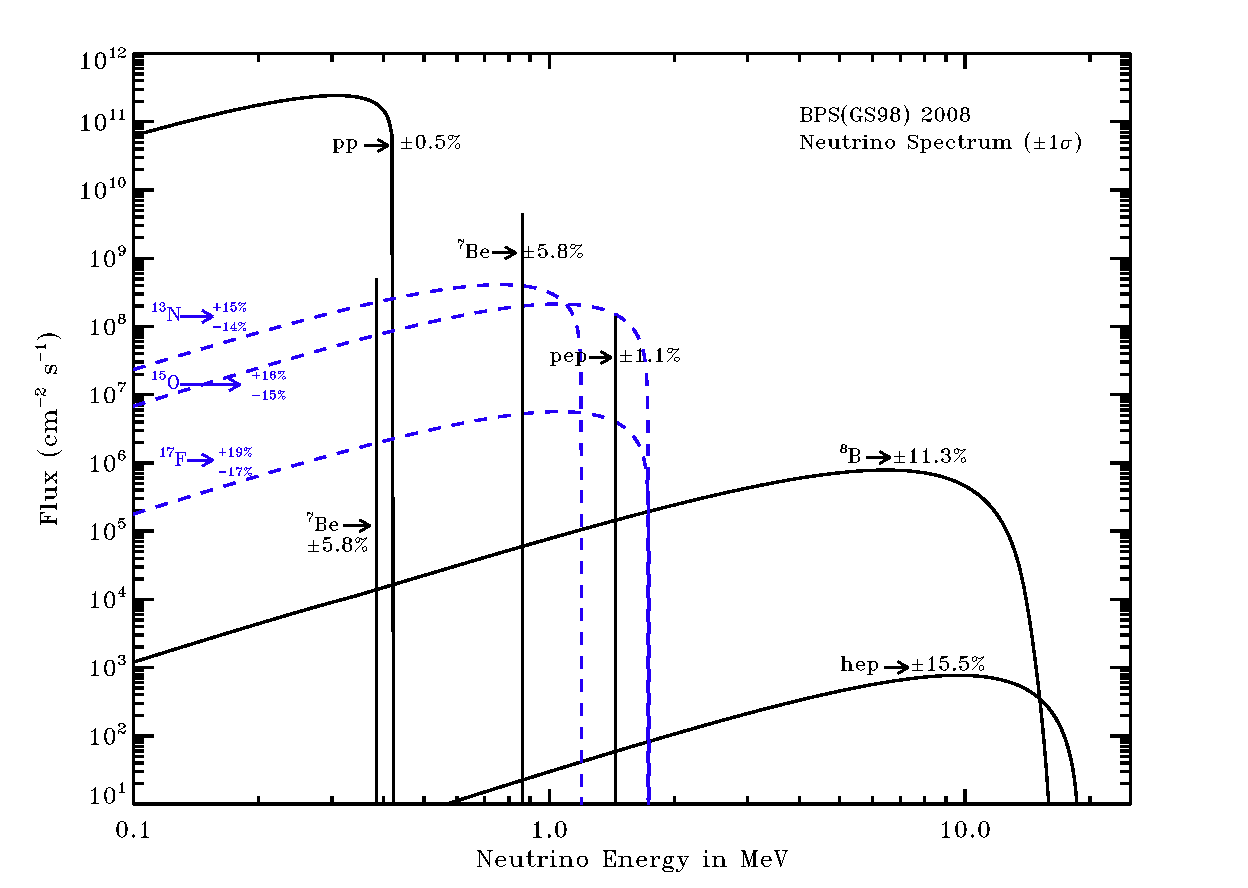
\includegraphics[width=0.6\linewidth]{figures/nu_spectrum1.pdf}
%  \caption{
%Solar neutrino spectra and SSM uncertainties \cite{serenellif}. 
%}
% \label{fig:sol-spectra}
% \end{figure}


\subsection{The early experiments}

The radiochemical detection of neutrinos using the reaction 
$\nu_e~^{37}Cl\rightarrow~^{37}Ar~e^-$ was first suggested by Bruno Pontecorvo in 1946~\cite{pontecorvo46}. This reaction has a threshold of 0.814 MeV and is therefore sensitive mainly to the $^8$B and $^7$Be solar neutrinos.

After previous experiments with this technique on surface, in 1965 Ray  Davis started  to construct a major experiment deep underground at Homestake (South Dakota), with 615~t of perchloroethylene (C$_2$Cl$_4$) that took data between 1968 and 2002.
The argon production rate induced by solar neutrino was 0.48 counts per day over a background of 0.09 counts per day due to the interactions initiated by highly energetic muons with nuclei (so called cosmogenics).
The $^{37}$Ar half-life of 35 days allows to expose the tank for a period of 60-70 days, followed by the efficient extraction of the produced argon by purging the liquid with helium.  
The isotope $^{37}$Ar decays by electron capture: 90 \% of these occur on the K-shell producing an average of 3.5 Auger electrons with 2.82 keV of total energy. Miniature gas proportional counters were developed to detect with high efficiency and purity these decays, achieving single-atom counting.
The efficiency of the whole extraction chain was calibrated injecting known quantities of other argon isotopes ($^{36}$Ar and $^{38}$Ar).  

The result of the Homestake chlorine experiment~\cite{cleveland} for the capture rate  is
\begin{equation}
(\sigma \phi)_{Cl} = 2.56 \pm 0.16 \pm 0.16 \: SNU
\end{equation}
where SNU is Solar Neutrino Units (a SNU equals 10$^{-36}$ captures/nucleus/second) while the prediction from the GS98-SFII solar model is $8.00 \pm 0.97$ SNU, that is the measured rate was about 30 \% of the predicted rate.  
Starting from the first result in 1968 this major deficit triggered a thirty years long debate, where many particle physicists were convinced that the SSM was not correct. Indeed the production rate of $ {^8}$B neutrinos depends critically on the temperature of the Sun core as T$^{22}$ and helioseismological data were not yet available at that time to confirm the validity of the SSM. 

\begin{table}
\caption{Solar neutrino detectors.}
\centering
\begin{tabular}{|c|c|c|c|c|c|}
  \hline
  Detector & Composition & Active mass & Threshold (MeV)  \\ 
  \hline
Homestake & C$_2$Cl$_4$ & 615t &  0.814 \\
Kamiokande & H$_2$O & 2.14kt &  7  \\
SAGE & Ga & 57t &  0.233 \\
GALLEX/GNO & Ga & 30.3t &  0.814  \\
Super-Kamiokande &  H$_2$O & 50kt &  3.5 \\
SNO & D$_2$O & 615 &  6\\
Borexino & C$_9$H$_{12}$ & 278t &  0.2  \\
  \hline
\end{tabular}

\label{tab:snudet}
\end{table}

It took more than twenty years before other radiochemical experiments could probe solar neutrinos~(Table~\ref{tab:snudet}). SAGE (1989-2007)~\cite{abdurashitov} in the Baksan Laboratory (Russia) and Gallex (1991-1997)~\cite{hampel}, followed by GNO (1998-2003)~\cite{altmann}, in the Gran Sasso Laboratory (Italy) used the reaction  $\nu_e  + {}^{71}{\rm Ga} \rightarrow {}^{71}{\rm Ge} + e^-$
that has a lower threshold, 0.233 MeV, and provides sensitivity to the $pp$ neutrinos, constituting the majority of the flux. 

While the details of these experiments, related to the chemical properties of gallium, is different from Homestake, they follow the same overall scheme of that experiment. They provided a confirmation of the solar neutrino deficit~\cite{abdurashitov,hampel,altmann,kaether}, although with a different reduction factor of approximately 50\% with respect the SSM prediction:
\begin{eqnarray}
(\sigma \phi)_{SAGE} & = & 65.4^{+3.1} _{-3.0} \; ^{+2.6} _{-2.8}  SNU \\
(\sigma \phi)_{GALLEX} & = & 73.4  ^{+6.1}_{-6.0} \; ^{+3.7} _{-4.1} SNU \\
(\sigma \phi)_{GNO} & = & 62.9  ^{+5.5} _{-5.3} \; ^{+2.5} _{-2.5} SNU 
\end{eqnarray}
to be compared with a predicted flux of 126.6 $\pm$ 4.2 SNU (GS98) (Fig.~\ref{fig:sol-spectra}).


\subsection{Real time experiments: Kamiokande, Super-Kamiokande, SNO, Borexino}

In 1987-1995 the 2.14 kt water Cherenkov experiment Kamiokande in Japan, in its phases II and III, provided a totally different measurement of the solar neutrinos flux. Neutrinos elastic scattering on electrons, mainly sensitive to electron neutrinos, could be detected with a threshold of 9 MeV, progressively reduced to 7 MeV.  
The water Cherenkov detection technique, also used later by the Super-Kamiokande and the SNO experiments, will be described in section~\ref{subsec:atmevidence}.   
Kamiokande was the first experiment to detect in real-time solar neutrinos. Since the scattered electron is emitted preferentially in the direction of the neutrino, it could verify their solar origin by correlating the electron momentum with the Sun direction. The combined result of Kamiokande~\cite{fukuda} is
\begin{equation}
\phi( ^8 B) = [2.80 \pm 0.19 (stat) \pm 0.33 (sys)] \times 10^6 {\rm cm^{-2} s^{-1}}
\end{equation}
providing another indication of a large suppression of the flux predicted by the solar model.

The 50kt water Cherenkov detector Super-Kamiokande, with a threshold of 7 MeV initially and today 3.5 MeV, started taking data in 1996 and confirmed the Kamiokande result with increased precision until its most recent update~\cite{abesk4}
\begin{equation}
\phi( ^8 B) = [2.308 \pm 0.020 (stat) ^{+0.040}_{-0.040} (sys)] \times 10^6 {\rm cm^{-2} s^{-1}}.
\end{equation} 

Super-Kamiokande is still running at present and it has recently observed for the first time a day-night effect for solar neutrinos~\cite{renshaw}. 
Let $r_D$ ($r_N$) be the day (night) event rate,
the day-night asymmetry $A_{DN}$ is defined as $A_{DN} = \frac{2 (r_D - r_N) }{r_D + r_N}$ and was measured to be
\begin{equation}
A_{DN} = (-3.2 \pm 1.1 (stat) \pm 0.5 (syst)) \%,
\end{equation} 
deviating from zero by 2.7 $\sigma$.
This is similar to $K_S^0$ regeneration for a beam of $K_L^0$ passing through a material. It is the first indication of Earth matter effects on neutrino propagation. 


%\begin{figure}[htbp]
%\centering
%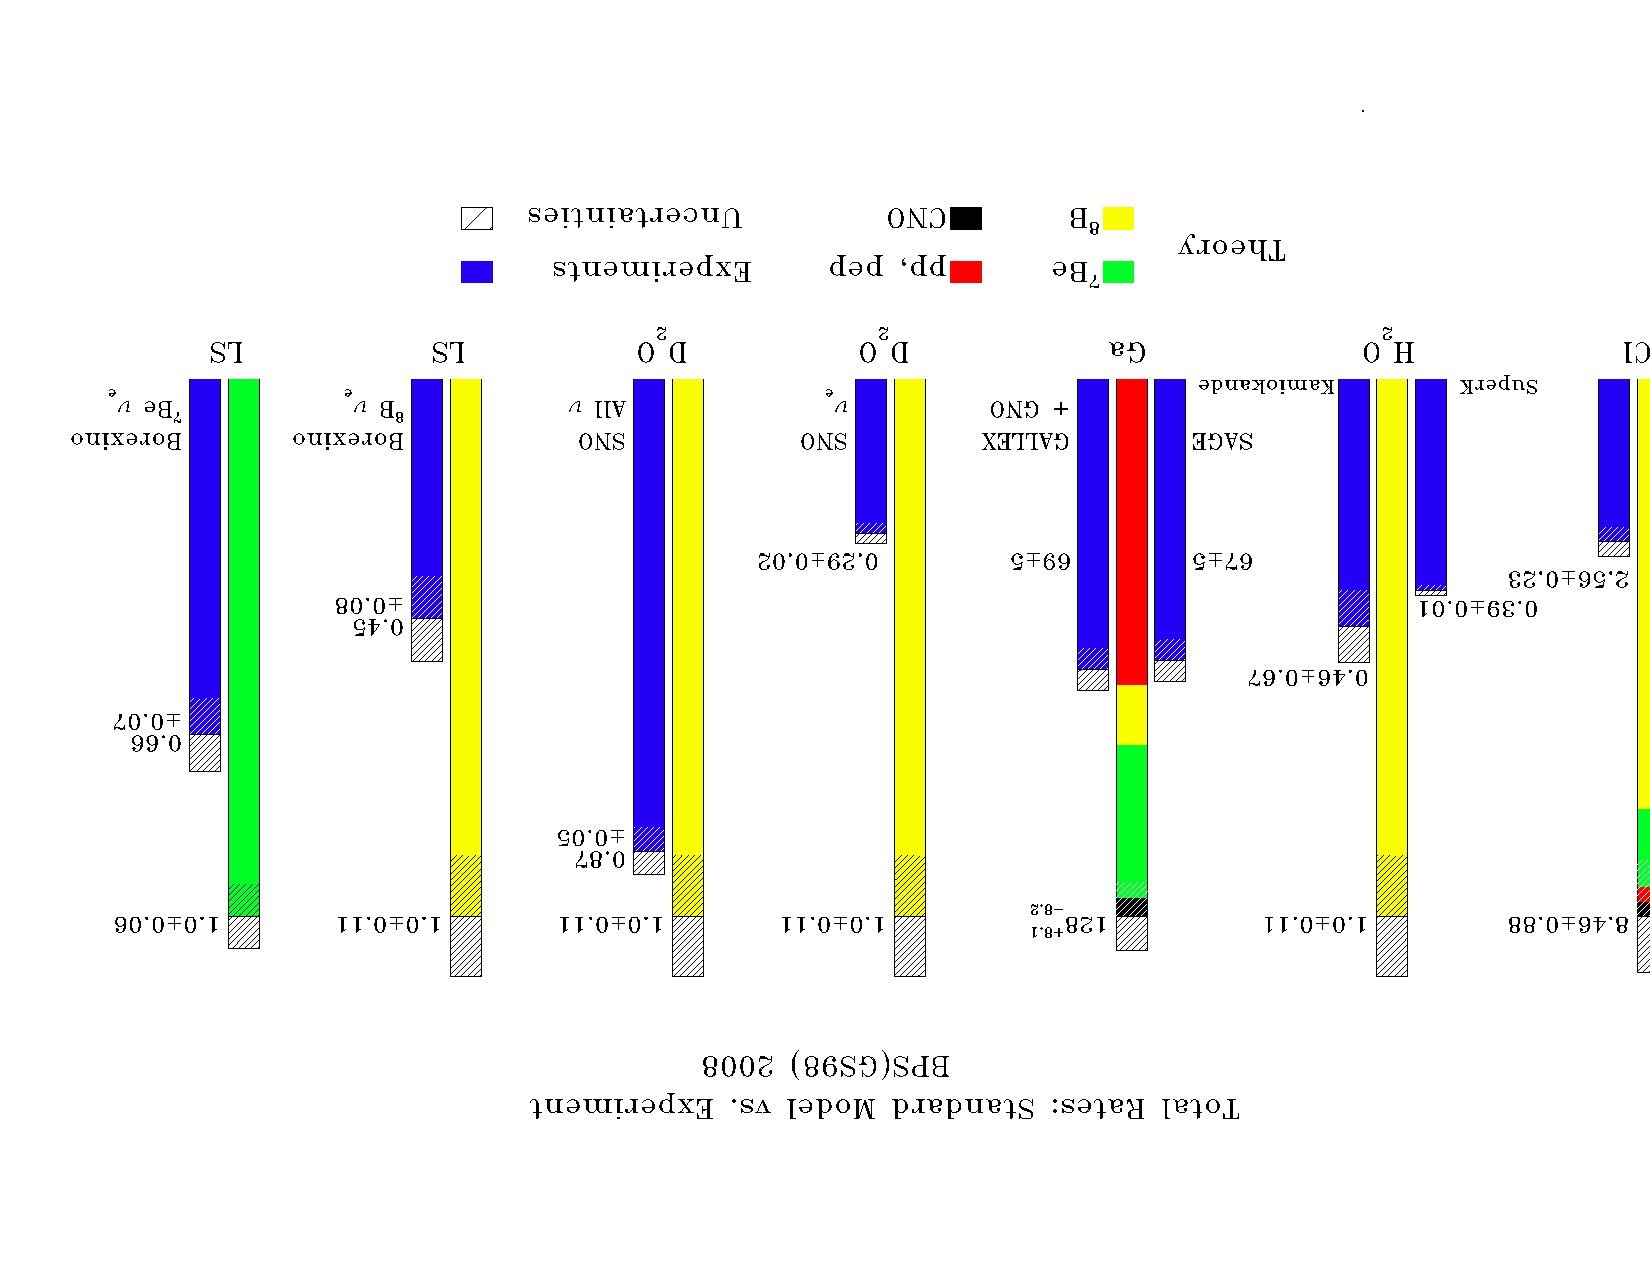
\includegraphics[angle=180,width=0.8\linewidth]{figures/theoryvsexpsnu1.pdf}
%  \caption{
%Measurements of the solar neutrino fluxes by various experiments compared to the SSM prediction~\cite{serenellif}.
%}
% \label{fig:sol-theoryexp}
% \end{figure}

The main limitations of the radiochemical and the water Cherenkov experiments is that they are only sensitive to charged current neutrino interactions with a \nue producing an electron in the final state. In this way it is not possible to distinguish between a deficit in the \nue flux due to a wrong SSM model prediction or a deficit due to neutrino oscillations.

The real breakthrough came from the Sudbury Neutrino Observatory (SNO, Canada), a Cherenkov detector 2 km below ground containing 1~kt of heavy water. 
With heavy water, three channels are available to probe the solar neutrino flux: 
\begin{itemize}
\item The charged current reaction for electron neutrinos $ \nu_e + d \rightarrow p + p + e^-$, where the produced electron carry off most of the neutrino energy allowing to constrain the neutrino spectrum;
\item The neutral current reaction $ \nu_x + d \rightarrow \nu_x +  p + n $ which allows to count all the neutrinos, independently of their flavour, above the threshold of 2.22 MeV; 
\item The electron scattering (ES) reaction $ \nu_x + e^- \rightarrow \nu_x + e^-$ also available in conventional water Cherenkov detectors, which is mainly sensitive to $ \nu_e$, as $\sigma_{ES}(\nu_e)\simeq 6 \; \sigma_{ES}(\nu_{\mu, \tau})$. 
\end{itemize}
SNO took data in three phases, distinguished by the technique used to detect the neutron produced in the neutral current dissociation of deuterium. Indeed, as the neutron is the only detectable particle in this reaction, this measurement is an experimental challenge and places severe requirements on the radiopurity of the whole apparatus. The different neutron detection techniques improved the sensitivity to the NC reactions. In the first phase neutron capture on deuterium was used. In the second phase, NaCl was dissolved in the water and neutrons were detected through the neutron capture on $^{35}$Cl followed by gamma emission. In the third phase neutron detectors containing $^3$He were inserted in the detector.
The electron kinetic energy threshold was 5 MeV, making the experiment sensitive to the ${}^8$B neutrinos. 
The results of all phases of the detector were in agreement and yielded a measurement of the total flux of solar neutrinos~\cite{aharmim}, irrespective of their flavour,
\begin{equation}
\phi_{NC} (\nu \; active ) = [5.25 \pm 0.16 (stat) ^{+0.11}
_{-0.13} (syst)] \times 10^6 {\rm cm^{-2} s^{-1}} 
\end{equation}
in agreement with the prediction of the solar models ($5.05 \times 10^6 {\rm cm^{-2} s^{-1}}$), and the flux of $\nu_e$
\begin{equation}
\phi_{CC} (\nu_e ) =  (0.301 \pm 0.033) \; \phi_{NC} (\nu \; active ).
\end{equation}
As we will discuss in section~\ref{subsec:solarinter} this is clearly an indication of flavour conversion of solar neutrinos. 

Finally another important experiment in the field of solar neutrino physics is the Borexino experiment that is running since 2007. Borexino is a 278~t liquid scintillator detector installed in the Gran Sasso Laboratory (Italy). 
It is capable of measuring low energy neutrinos with a threshold of 200 keV in real time, thanks to the high light yield of 10$^4$ photons per MeV which is much higher than in a Cherenkov detector and to the extreme levels of radiopurity reached inside the scintillator tank. 

Combining these two features Borexino was able to measure the flux of neutrinos from different reactions: the original goal of the experiment was the measurement of the $^7$Be neutrino flux that was measured to be $(3.10 \pm 0.15) \times 10^9 {\rm cm^{-2} s^{-1}}$ corresponding to the 62 \% of the GS98 SSM predicted flux~\cite{bellini}. It also provided the first determination of the pep flux 
$(1.6 \pm 0.3) \times 10^8 { \rm cm^{-2} s^{-1}}$ and a measurement of $^8$B neutrinos with a 3~MeV threshold. 
Finally they recently published the first real time observation of $pp$ neutrinos 
%measuring a flux, assuming LMA-MSW solution, of $(6.6\pm0.7)\times10^{10}{ \rm cm^{-2} s^{-1}}$ 
as well as the most stringent upper limit on the CNO neutrino flux. This is interesting since the flux of CNO neutrinos is sensitive to the assumption on the metallicity for the SSM.


\subsection{Confirmation with reactor neutrinos: KamLAND}

KamLAND is a 1~kt liquid scintillator experiment located in the former site of the Kamiokande detector in Japan. As described in more detail in section~\ref{subsec:reactorflux}, it is capable of detecting $\bar \nu_e$ emitted by nuclear reactors through the inverse beta decay reaction $\bar{\nu}_e \; p \rightarrow n \;  e^+$. KamLAND is surrounded by 55 Japanese nuclear reactors at an average distance of 150 km. In 2002, it reported first evidence for the disappearance  of $\bar \nu_e$. This measurement was very important for the interpretation of solar neutrino data as it showed for the first time an oscillatory behaviour as a function of L/E and it provided an independent and precise measurement of the oscillation parameters of interest.
In an updated report in 2013~\cite{Gando:2013nba}, they observed 2611 
events to be compared to $3564 \pm 145$ expected from reactor neutrinos in the case of no oscillation and  $364.1 \pm 30.5$ from background sources.
The KamLAND results are shown in Fig.~\ref{fig:sol-kam}. 

\begin{figure}[htbp]
\begin{minipage}[c]{.46\linewidth}
%\begin{minipage}[c]
   	      \includegraphics[width=0.9\linewidth]{figures/kamland_LE1.pdf}
   \end{minipage} \hfill
   \begin{minipage}{.46\linewidth}
      \includegraphics[width=0.9\linewidth]{figures/kamland_dmth1.pdf}
   \end{minipage}
    \caption{KamLAND experiment. The left plot shows the ratio of the background and geo-neutrino-subtracted $\bar{\nu}_e$
spectrum to the expectation for no-oscillation as a function of
L/E. The curve and histograms show the expectation for the best fit oscillation hypothesis. The right plot shows the allowed region for neutrino oscillation parameters from
KamLAND and solar neutrino experiments~\cite{Gando:2013nba}. Courtesy of the KamLAND collaboration.} 
 \label{fig:sol-kam}
\end{figure}


\subsection{Interpretation of the measurements and discussion}
\label{subsec:solarinter}

The first measurement of a deficit of the solar neutrino flux left open several interpretations. While early on Pontecorvo made the hypothesis of neutrino oscillations~\cite{Pontecorvo:1967fh}, modest changes to the Sun core temperature could also be invoked to explain the apparent deficit. 
The situation changed with the new measurements by the gallium experiments, as it was clear that the suppression factor depended on the neutrino energy. The SNO results were the first measurement of the total solar neutrino flux and were also the first solid proof of flavour conversion as the explanation of the solar neutrino puzzle. 

Nevertheless, several different solutions were possible in the early days in terms of masses and mixing. The KamLAND result pinpointed one of them, the so-called Large Mixing Angle (LMA) solution which was already favoured by SNO data. Indeed, the results of KamLAND can be understood in terms of a simple two neutrino mixing formula $ P(\bar{\nu}_e \rightarrow \bar{\nu}_e ) = 1 - \sin^2 2 \theta_{12} \sin^2 (\frac{\Delta m^2_{21} L}{4 E}) $, neglecting matter effects and effects related to $\theta_{13}$ (cf. Eq.~(\ref{eq:nuereactor})). 

As we will see later, the value of $\Delta m^2_{31}$ is much larger than $\Delta m^2_{21}$ and induces rapid oscillations that are averaged out given the large $L/E$ and the energy resolution of that experiment. The $L/E$ pattern is prominent in the KamLAND data and beautifully confirms neutrino oscillations as the origin of the observed deficit (Fig.~\ref{fig:sol-kam}). The measurement of KamLAND, when combined with solar neutrino experiments, allows to determine $\Delta m^2_{21} = (7.53 \pm 0.18) \times 10^{-5} eV^2$ and $\tan^2 \theta_{12} = 0.44 \pm 0.03$. The agreement between solar neutrino experiments and KamLAND is good, as shown in Fig.~\ref{fig:sol-kam}.

The explanation of the deficit observed by the solar neutrino experiments involves flavour transitions of a different kind. As explained in section~\ref{subsec:varying}, electron neutrinos are produced in the core of the Sun in a medium of high density. 
In the center of the Sun, the density $n(r=0)$ corresponds to the resonant density $ n_{res}= \frac{\Delta m^2_{21} \cos 2 \theta_{12}}{ 2 \sqrt{2}G_F E}$ for E = 1.9 MeV. For energies much higher than this value
%If the condition $n(r) > n_{res}= \frac{\Delta m^2_{21} \cos 2 \theta_{12}}{ 2 \sqrt{2}G_F E}$ is satisfied, corresponding to energies above 3.3 MeV for pp, 2.2 MeV for $^7$Be and 1.8 MeV for $^8$B neutrinos, 
neutrinos are produced as the $ \nu^m_2$ matter eigenstates of the Hamiltonian and in its adiabatic evolution exits the Sun as $\nu_2$. The probability to observe them as $\nu_e$ is then $\sin^2 \theta_{12} \sim 0.3$. 

For neutrinos produced with energies much below this threshold, matter effect can be neglected and they undergo vacuum oscillations. The suppression factor observed on Earth is then the result of the averaging of many oscillation periods    
$ P({\nu}_e \rightarrow {\nu}_e ) = 1 - \frac{1}{2} \sin^2 2 \theta_{12} \sim 0.58$. 
This leads to a characteristic "bath tub" shape for the neutrino survival probability (Fig.~\ref{fig:sol-bor}). The adiabatic flavour conversion dominates for $^8$B neutrinos, while pp are in the average vacuum oscillation region. 
%The measurement of pep neutrinos would be interesting as they are in the transition region.
This interpretation fits with all the solar neutrino data. 

The future of this field is twofold. The solar neutrino experiments will try to measure the CNO neutrinos as this is both interesting {\it per se} (the original motivation to study the solar neutrinos was in fact to understand how the Sun shines) and it will shed some light on the solar abundance problem. This will be attempted by Borexino and SNO+~\cite{snoplus}, with liquid scintillator instead of the heavy water in the inner vessel. 

The upturn of the solar neutrino survival probability, that is the transition from the MSW to the vacuum oscillation regime, in the few MeV region, is predicted by the MSW model, however it has not yet been observed. 
Experimentally this is very difficult as it requires to lower the threshold and to have a good control of the backgrounds. The failure so far to observe this upturn is also related to the mild tension reported by global fits of neutrino properties between the $\Delta m^2_{21}$ measured by KamLAND and the measurement using solar neutrino data~\cite{nufit}. Precision measurements of the solar neutrino flux are also a powerful probe of new physics scenarios.
 
On the other hand the long baseline reactor experiment JUNO, using the same technique as KamLAND, with 20~kt liquid scintillator will dramatically improve the precision, below the percent level, on the solar oscillation parameters  $\Delta m^2_{21}$ and $\theta_{12}$.

\begin{figure}[htbp]
\centering
\includegraphics[width=0.6\linewidth]{figures/pee.pdf}
  \caption{
  Solar neutrino survival probability as a function of the energy with the Borexino results \cite{derbin2016}. The gray band correspond to the $\pm1\sigma$ prediction of the MSW-LMA solution. Courtesy of the Borexino collaboration.
}
 \label{fig:sol-bor}
 \end{figure}


\clearpage
%% Atmospheric sector
\section{The 2-3 atmospheric sector }

In this subsection we will describe the status of the so called atmospheric neutrino oscillations, i.e. the 2-3 oscillations that were first discovered in the study of atmospheric neutrinos and later were precisely measured with the use of long baseline neutrino beams.   


\subsection{The atmospheric neutrino flux}

The atmosphere is constantly bombarded by primary cosmic rays, composed mainly of protons, with a smaller component, $\simeq$ 5\%, of $\alpha$ particles, and even smaller fraction of heavier nuclei. The interaction of these particles with atomic nuclei in the atmosphere produces hadronic showers composed mainly of pions and kaons. The decay of these mesons according to 
$\pi^+ \rightarrow \mu^+ \nu_\mu$ followed by 
$\mu^+ \rightarrow e^+ \nu_e \bar{\nu}_\mu $,
$K^+ \rightarrow \pi^+ \nu_\mu$ and $K_L \rightarrow \pi^+ e^- \nu_e$
together with their charge conjugated processes produces a flux of $\nu_\mu$ and $\nu_e$ with a steeply falling power-law spectrum (Fig. \ref{fig:nuatmflux}), approximately $E^{-2.7}$ in the region above 1 GeV.   


\begin{figure}[htbp]
\begin{minipage}[c]{.46\linewidth}
%\begin{minipage}[c]
   	      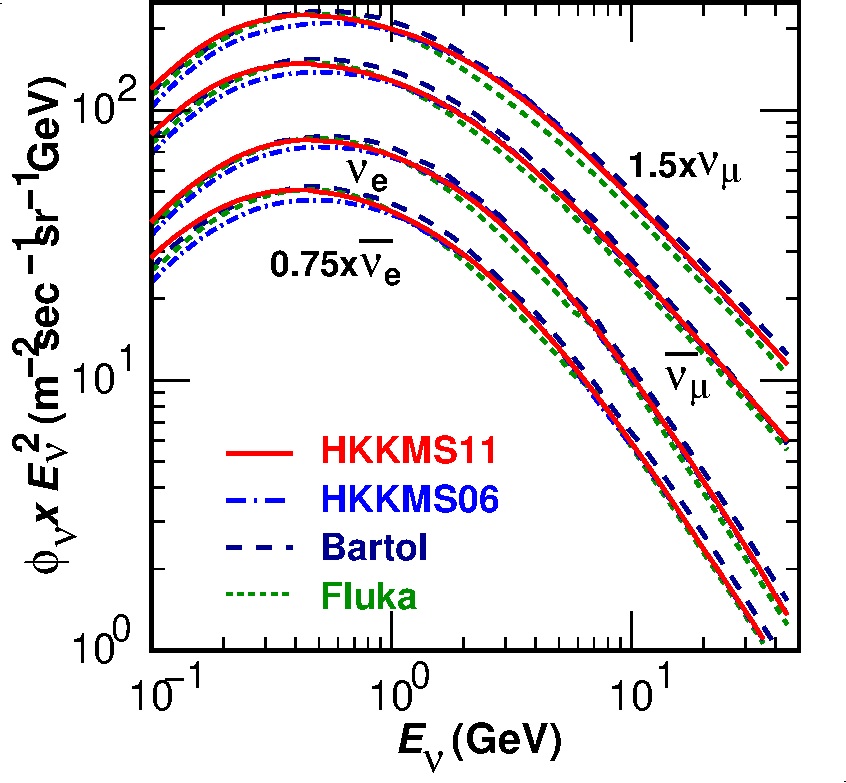
\includegraphics[width=0.9\linewidth]{figures/fig7a-c.pdf}
   \end{minipage} \hfill
   \begin{minipage}{.46\linewidth}
      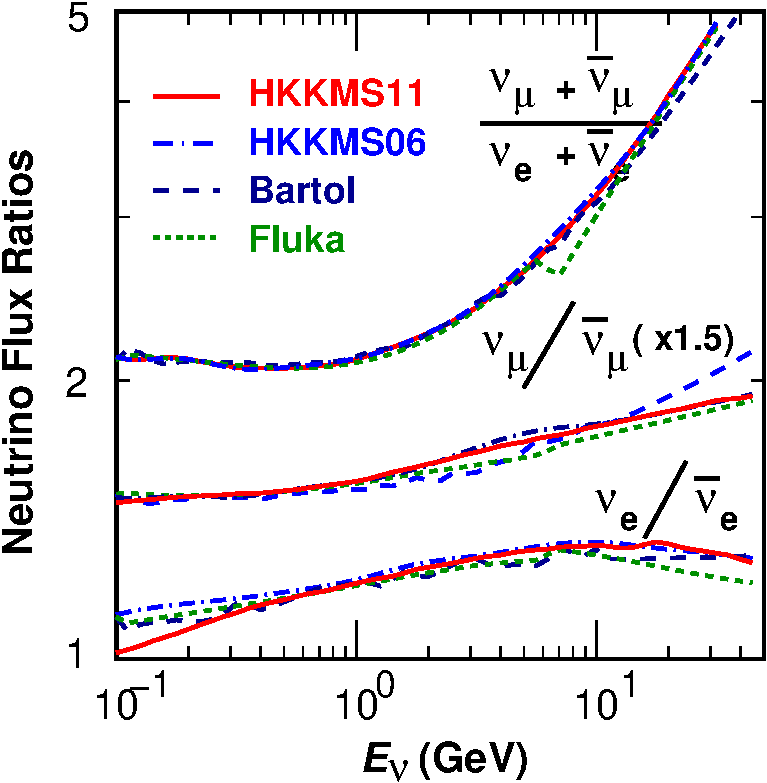
\includegraphics[width=0.9\linewidth]{figures/fig7b-c.pdf}
   \end{minipage}
    \caption{The flux of atmospheric neutrinos (left) and several flux ratios (right) \cite{PhysRevD.83.123001}. }
 \label{fig:nuatmflux}
\end{figure}


The calculation of this neutrino flux \cite{Gaisser:2002jj} relies on the knowledge of the primary flux and composition, of the Earth magnetic field, and of the hadro-production cross-section. Recent studies \cite{PhysRevD.83.123001,Barr:2004br,Battistoni:2002ew} taking into account 3D effects and recent measurements of the hadro-production cross-sections largely improve on previous efforts and reach precisions of 7-8 \% for the flux in the 1-10 GeV range. It should be noticed that the ratio $N(\nu_\mu + \bar{\nu}_\mu)/N(\nu_e + \bar{\nu}_e)$ is predicted with a much better precision of a few \% as several systematic uncertainties cancel in this ratio. In the limiting case where all the muons from pion decays decay themselves in flight, this ratio is close to 2, as can be easily deduced from the decay processes mentioned above.

%\subsection{The early days, the up-down asymmetry and controversy}

\subsection{Interaction of high energy neutrinos with the nucleus}

The interaction of neutrinos with matter takes place through charged current (CC) interactions (exchange of a $W$ boson, production of a charged lepton in the final state) or neutral current (NC) interactions (exchange of a $Z^0$ boson). 
Above a few hundred MeV neutrino energy interactions with the nucleus have a typical $q^2$ which is of the order of one fermi, and the neutrino scatters off individual nucleons inside the nucleus. These interactions (Fig.~\ref{fig:xsec}) can be classified as:
\begin{itemize}
  \item (Quasi-) Elastic interactions, where the finale state nucleon is ejected from the nucleus as a proton or neutron, 
  \item excitation of a nucleon resonance like the $\Delta$,
  \item Deep Inelastic scattering at large energies and for large momentum transfers, where the neutrino interacts with the partons inside the nucleons.
  \end{itemize}  

The Charged Current Quasi elastic process $\nu_l \: n \rightarrow l \: p$ where $l=e,\mu$ plays a special role because it is the dominant process below 1 GeV. Moreover its simple final state is very suitable to the reconstruction of the neutrino energy based on the measurement of the outgoing charged lepton. Neglecting Fermi momentum, the reconstructed neutrino energy is 
\begin{equation}
E_\nu = \frac{m_p^2 - (m_n-E_b)^2 - m^2_l + 2 (m_n-E_b)E_l}{2 (m_n - E_b - E_l + p_l \cos \theta)}
\end{equation}
 where $E_b$ is the effective binding energy necessary to extract the nucleon from the nucleus, $m_p$ $m_n$ and $m_l$  are the proton, neutron and lepton mass, $E_l$, $p_l$ and $\theta$ are the reconstructed lepton energy, momentum and angle with respect to the beam. This process is particularly suited for Cherenkov detectors, because, while the proton and most of the pions in these interactions are below the detection threshold, electrons and muons can be easily detected, reconstructed and identified. 

In the simplest approach to the calculation of the cross-section, the nucleus is simply parametrized by the Fermi momentum and the binding energy $E_b$. The CCQE cross-section is then mainly governed by the axial vector form factor of the nucleon, where usually a dipole form is assumed
$ G_A (q²) = \frac {g_A} {(1+q²/M²_A)}$.
Most parameters are determined from electron scattering for the vector from factors, and from nuclear $\beta$ decays for $g_A$, leaving the axial mass value $M_A$ as the main free parameter. This simple approach failed, as revealed by the fact that the value of $M_A$ 1.2-1.3 GeV/c$^2$ measured by K2K and  MiniBoone for interactions on carbon was very different from the value 1.03 GeV/c$^2$ obtained from the analysis of neutrino interactions on deuterium (Fig.~\ref{fig:xsec}).

\begin{figure}[htbp]
\begin{minipage}[c]{.46\linewidth}
%\begin{minipage}[c]
   	      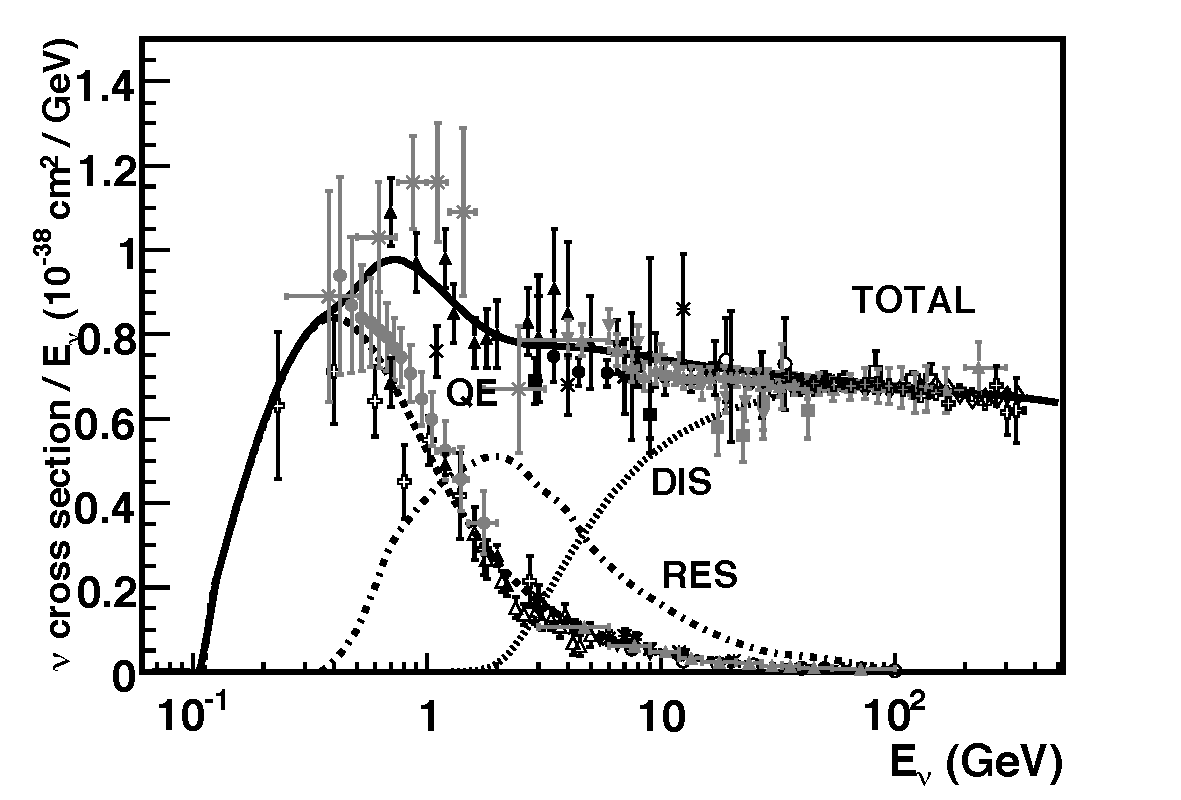
\includegraphics[width=0.9\linewidth]{figures/cc_inclusive_nu.pdf}
   \end{minipage} \hfill
   \begin{minipage}{.46\linewidth}
      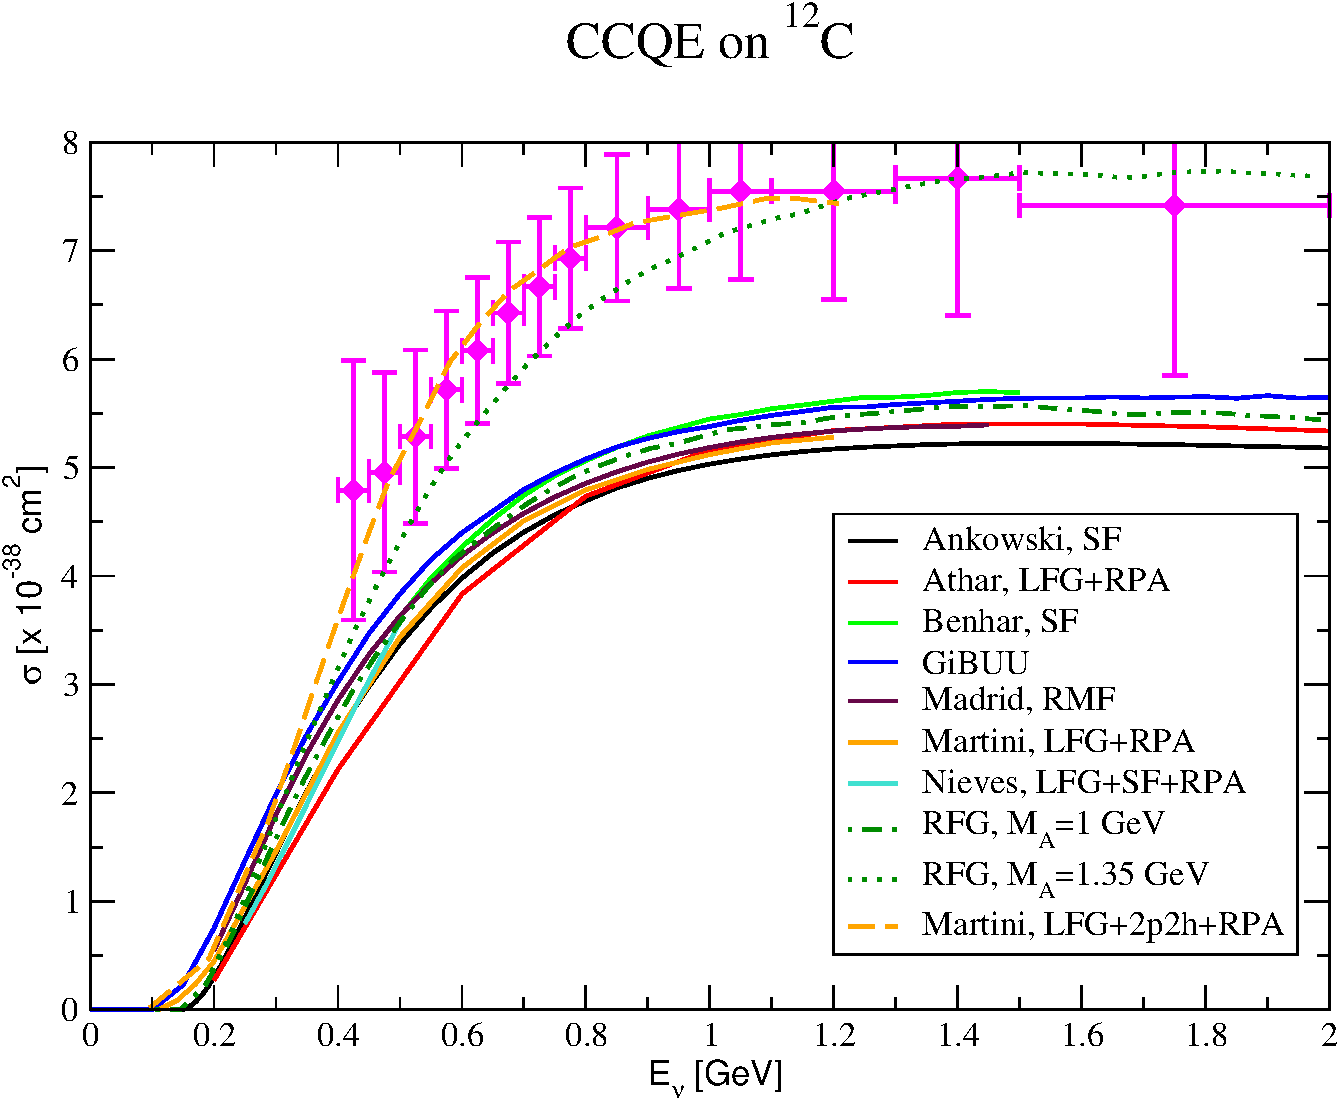
\includegraphics[width=0.9\linewidth]{figures/CCQE_C_2.pdf}
   \end{minipage}
    \caption{ Left plot: Total neutrino per nucleon CC cross sections (for an isoscalar target) divided by neutrino energy and
plotted as a function of energy~\cite{formaggio}.
Right plot: CCQE cross-section on carbon~\cite{alvarez}.
The solid
lines denotes various models.  The dash-dotted and
dotted lines are two models with $m_A=1$ and 1.35 GeV respectively. 
The dashed line takes into account the 2p-2h.  The data points
are from MiniBooNE.}
 \label{fig:xsec}
\end{figure}

A partial solution to this discrepancy came from considering additional processes like interactions of the neutrino with a correlated pair of nucleon inside the nucleus. These processes are known to exist in electron-nucleus scattering. From the experimental point of view, these processes, named two particle-two hole (2p-2h), cannot be distinguished from CCQE interactions, as low momentum protons and neutrons are generally not detected. These processes can represent 10-20 \% of the CCQE cross-section. Despite this progress, the normalization and shape of this additional contribution is still not well-known and model-dependent.

Other nuclear effects, like Final State Interactions (where the ejected nucleon reinteracts within the same nucleus), or Secondary Interactions (where the nucleon interacts with other nuclei in the detector) introduce smearing and corrections which are under evaluation, especially for relatively large nuclei like Carbon, Oxygen, Argon and Iron generally used in these experiments. 
The anti-neutrino cross-sections are even less established with less precise measurements, as it is the case for the $\nu_e$ cross-sections required by the oscillation experiments.  

All these cross-sections are the object of an intense theoretical and phenomenological activity \cite{zeller,martini} given their relevance for oscillation analyses. The knowledge of these cross-sections is still model-dependent and the precision does not exceed the 10-20 \% level. Therefore, most of the experiments include near detectors to study the event rates before oscillations intervene. Clearly a more focused effort, combining phenomenological developments and well controlled experimental data is required for future high precision oscillation experiments.


\subsection{The evidence for atmospheric neutrino disappearance}
\label{subsec:atmevidence}
%from Super-Kamiokande}

The study of atmospheric neutrinos started in the 1960: two experiments in very deep mines, in South Africa \cite{Reines:1965qk} and in India \cite{Achar:1965ova}, observed muons produced by their interactions. 
In the 1980, several massive underground experiments, mainly motivated by the search for the proton decay predicted by Grand Unification theories, started collecting data. These experiments needed to study in detail atmospheric neutrino interactions as they constitute a background for proton decay searches.

In 1988, Kamiokande~\cite{kam88} reported a deficit in the number of $\nu_\mu$ of events (85 $\pm$ 9.2 observed versus 144.5 expected), while the number of $\nu_e$ events agreed with the prediction (93 $\pm$ 9.6 observed versus 88.5 expected). 
This initiated the so-called atmospheric neutrino anomaly. A similar deficit was also observed by the IMB experiment and later by MACRO and SOUDAN-2, while Fr\'ejus and NUSEX observed no deficit. 

The situation evolved rapidly with the advent of Super-Kamiokande~\cite{sknim}, that started data-taking in 1996. Super-Kamiokande is very large water Cherenkov detector located in the Mozumi mine (Gifu prefecture, Japan), under a 1000 m rock overburden, equivalent to 2700 m of water. It is a stainless steel tank (41.4 m high, 39.3 m diameter) containing 50 kt of ultra-pure water. The detection volume is partitioned in an outer detector, composed of 1885 8 inch PMTs, and an inner detector with 11146 20 inches PMTs. The fiducial volume is 22.5 kt. Super-Kamiokande could rapidly accumulate a rather large data set of atmospheric neutrinos, measuring the direction of the produced lepton, its energy for fully contained events and their nature. Above a few hundred MeV/c, the direction of the produced lepton is strongly correlated to the direction of the incoming neutrino.

Super-Kamiokande classifies events as Fully Contained (where the neutrino interaction takes place inside the inner detector and all the particle stop in the same volume), Partially Contained (some particles escape to the outer detector) and Upward Going muons, where the neutrino interacts in the rock below the detector. The events can be further classified according to the number of Cherenkov rings observed, the observed total energy, the number of decay electrons. Electrons and muons can be reliably identified (the misidentification probability is 0.7 \%) on the basis of the ring properties. Cherenkov rings produced by muons have sharp edges while in the case of electrons the photons are produced by the numerous electrons and positrons in the electromagnetic shower, with angular dispersion due to scattering, resulting in a ring with diffuse edges. The momentum resolution for isolated ring produced by a lepton of momentum $p$ is $0.6\% +2.6\%/\sqrt{p ({\rm GeV/c})}$. Sub-threshold muons and charged pions can be tagged by the presence of a delayed electron from muon decay.

In 1998, the Super-Kamiokande collaboration presented their first analysis of atmospheric neutrinos~\cite{Fukuda:1998mi}, in particular the distributions of zenith angle for $ \nu_\mu$ and $\nu_e$ event selections (see Fig.~\ref{fig:sk-atm} for an updated distribution) based on an exposure of 33 kton year. This was the first compelling evidence for neutrino oscillations as the explanation of the previously mentioned anomaly.  

Indeed the neutrino path from the production to the detection varies from 15 km for down-going neutrinos (cosine of the zenith angle equal to 1) to more than 12000 km for up-going neutrinos having traversed the whole Earth (cosine of the zenith angle equal to -1), thereby probing a large span of possible oscillation lengths. 

In a two neutrino scenario, the $\nu_\mu$ disappearance is governed by 
\begin{equation}
P(\nu_\mu \rightarrow \nu_\mu) = 1 - \sin^2 (2 \theta) \sin^2 (4 \Delta m^2_{atm} L /E),
\end{equation}
where $\theta$ is the relevant mixing angle and $\Delta m^2_{atm}$ the effective squared-mass difference of the mass eigenstates. A glance at Fig.\ref{fig:sk-atm} reveals several important overall features: 
\begin{itemize}
\item there is a strong disappearance of $\nu_\mu$, especially visible for up-going neutrinos. As the survival probability for very long baseline approaches $1- 1/2 \sin^2 (2 \theta)$, and the observed survival probability is close to 0.5, the mixing angle is therefore close to the maximal value $\pi/4$. 
\item The disappearance sets in for neutrinos close to horizontal zenith angle, and therefore the oscillation length should be of the order of 400 km for energy around 1 GeV, or $\Delta m^2_{atm} \simeq 10^{-3}$eV$^2$.  
\item There is no sizeable excess or deficit of $\nu_e$. Therefore the oscillations of $\nu_{\mu}$ should mainly involve either $\nu_{\mu} \rightarrow \nu_{\tau}$ or $\nu_{\mu} \rightarrow \nu_s$, where $\nu_s$ is an additional neutrino state.
\end{itemize}


\begin{figure}[htbp]
\centering
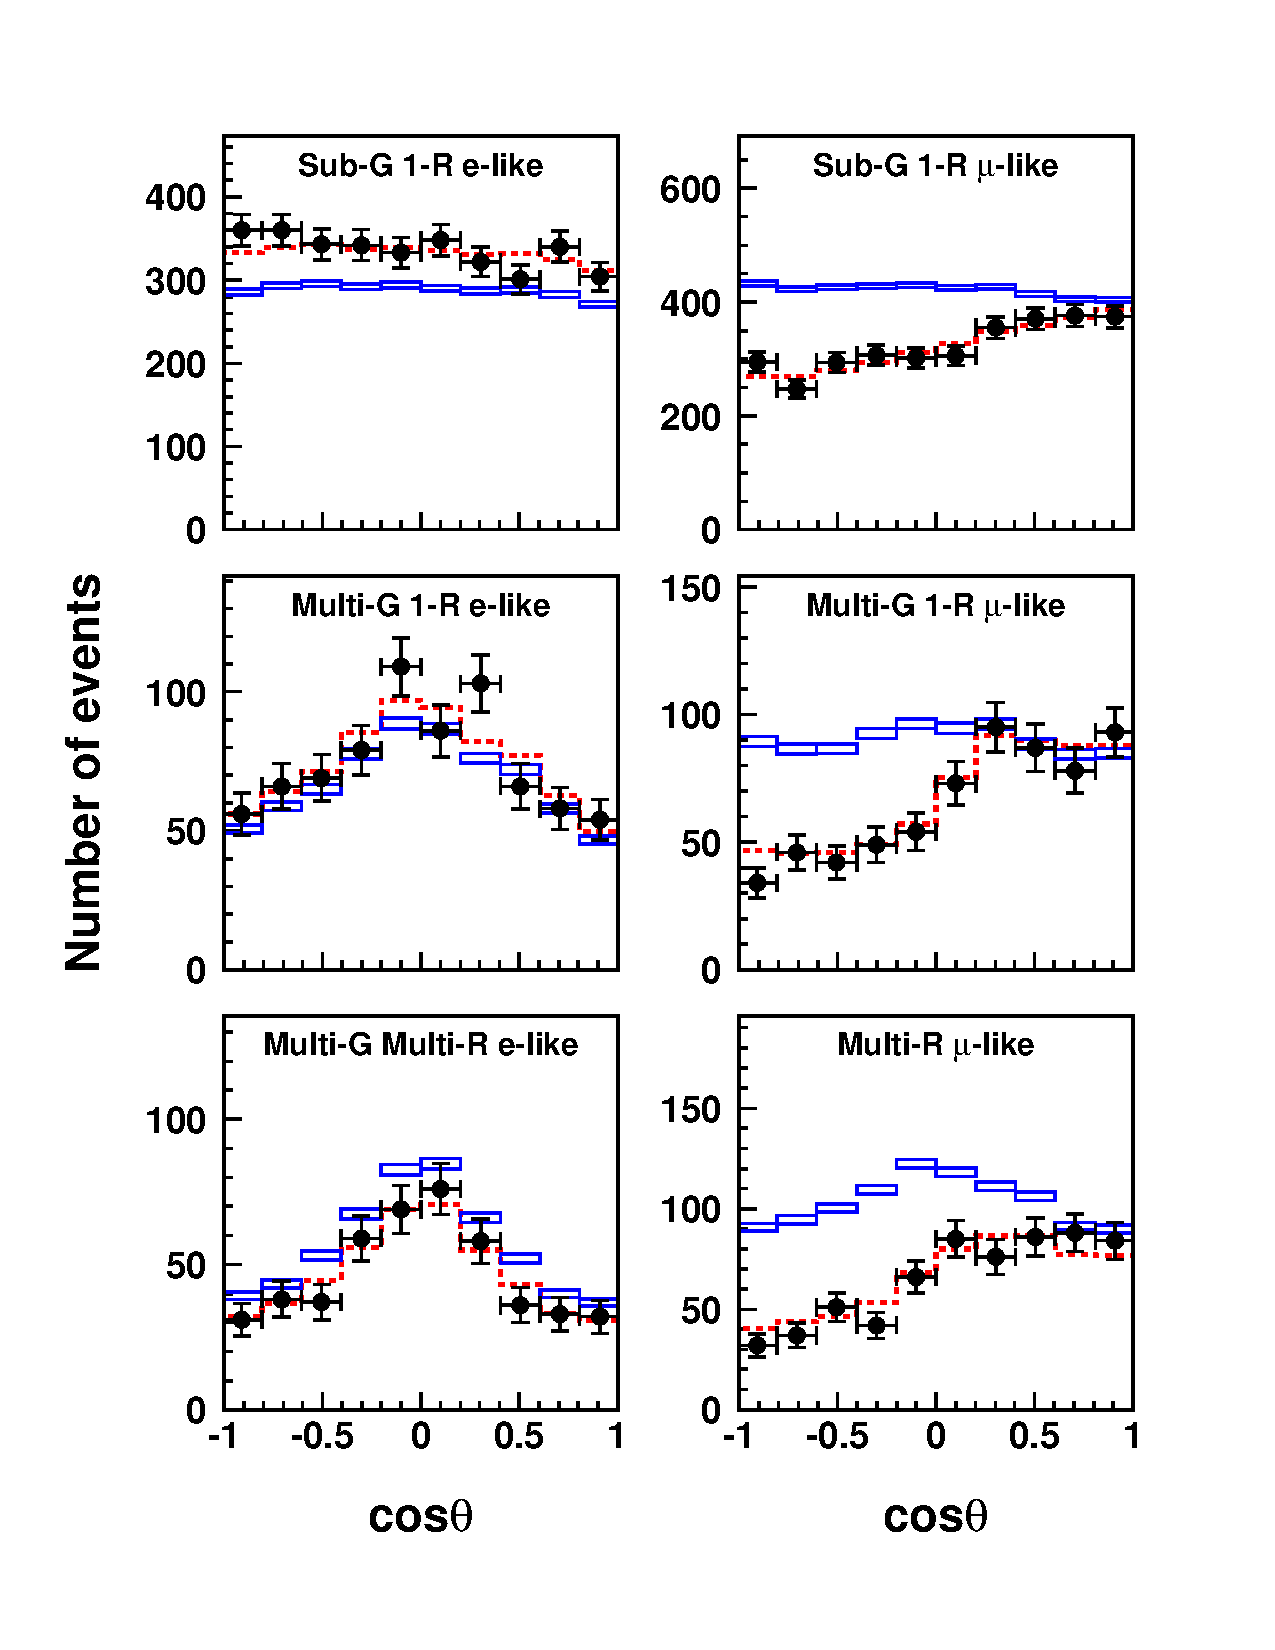
\includegraphics[width=0.8\linewidth]{figures/sk-2006-atm.pdf}
  \caption{Zenith angle distributions of Super-Kamiokande atmospheric neutrino events from \cite{Hosaka:2006zd}. Fully contained
e-like, $\mu$-like events
are shown for data (filled circles with statistical
error bars), MC distributions without oscillation (boxes)
and
best-fit distributions (dashed). The box height shows the
statistical error.}
 \label{fig:sk-atm}
 \end{figure}

Independently of any accurate predictions of the neutrino flux, the experimental observation of the distributions of Fig.\ref{fig:sk-atm} is sufficient to make a strong case for neutrino disappearance. Indeed, above several GeV, the neutrino flux is isotropic, as the primary cosmic rays are not deflected in a significant way by the geomagnetic field. The observation of a zenith angle dependent deficit of the neutrinos is then a sufficient argument to conclude that these neutrinos undergo a non-standard propagation.  

While in 1998 other hypotheses like decay or decoherence were still open, more recent data from long baseline accelerator experiments have ruled out all explanations apart from oscillations because the alternative hypotheses imply a different L/E behaviour. 
    
The IceCube experiment at the South Pole has recently completed the installation of DeepCore, a denser array of optical modules, aimed at significantly lowering the muon threshold. With data recorded between 2011 and 2014, corresponding to 5074 observed events, they have recently published an analysis of the disappearance of atmospheric $\nu_\mu$  \cite{Aartsen2016161} in the range 10-100 GeV, requiring the zenithal angle to satisfy $\cos \theta < 0$,  which has a similar sensitivity to that of Super-Kamiokande (Fig. \ref{fig:icecubeosc}) with the prospects of further improvements. 


\begin{figure}[htbp]
\centering
%\includegraphics[width=0.5\linewidth]{energy_miniboone.eps}
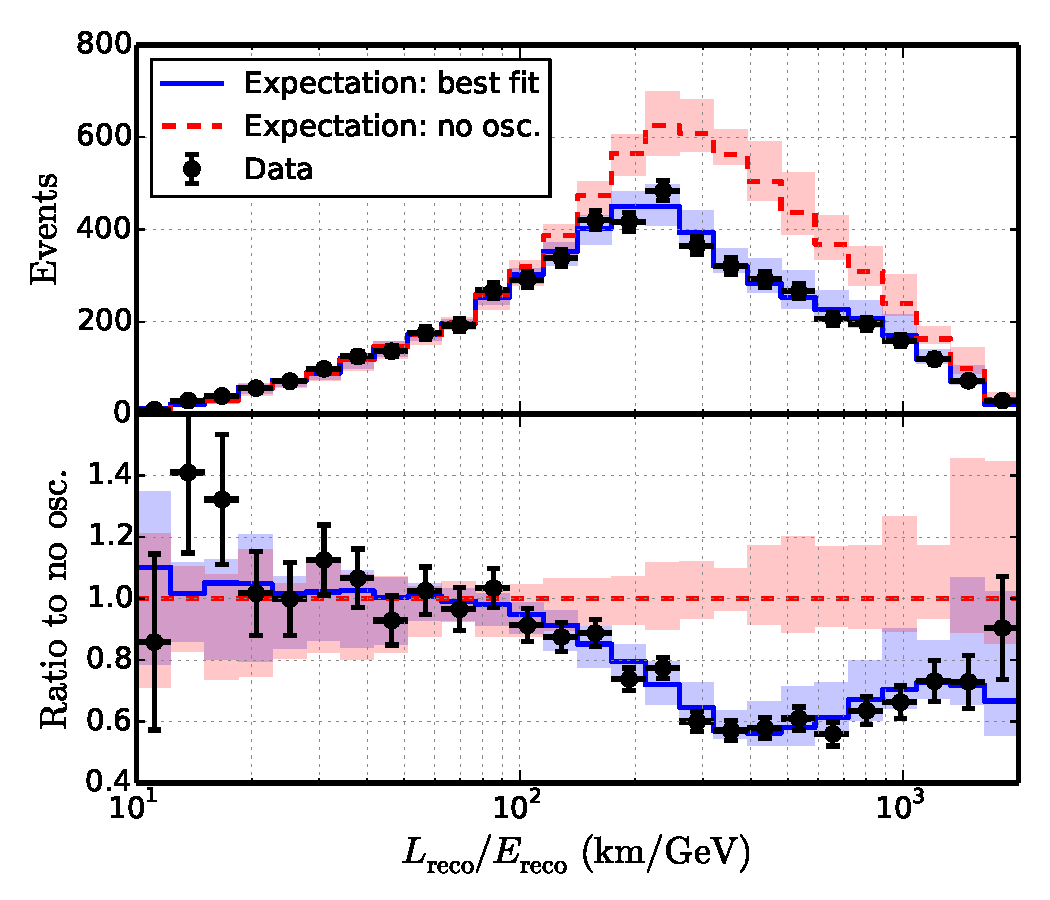
\includegraphics[width=0.6\linewidth]{figures/icecube_osc2014_data_mc_LE.pdf}
  \caption{Distribution of atmospheric neutrino events measured by the IceCube experiment\cite{Aartsen2016161} as a function of
reconstructed L/E. Data are compared to the best fit and
expectation with no oscillations (top), and the ratio of data
and best fit to the expectation without oscillations is also shown
(bottom). Bands indicate estimated systematic uncertainties.}
 \label{fig:icecubeosc}
 \end{figure}

%\newpage
%% Long baseline
\subsection{Long-baseline neutrino beams }

Neutrino beams~\cite{Kopp2007101} based on particle accelerators have been used since the 1960s, when they provided the evidence for the existence of two types of neutrino, $\nu_e$ and $\nu_\mu$. The general design is based on a high intensity proton beam impinging on a target and producing pions and kaons through interactions on the target nuclei. 
These mesons decay in a dedicated volume downstream of the target, creating mainly a $\nu_\mu$ beam.  

The long baseline beams are based on the so called wide band beam concept. Here the secondary charged mesons are focused using a system of magnetic devices, called horns. The horns, usually with a cylindrical symmetry around the beam, are pulsed with a very intense current in coincidence with the arrival of the beam. 
%The ratio between the primary proton energy and the typical neutrino energy is %at least a factor ten, and the neutrino spectrum extends for about a decade %around this typical energy.  

The flux is tuned in such a way that the phase $\Delta m^2_{32} L/ (4 E)$ reaches $\pi/2$ for the design baseline $L$ and the peak energy $E$, in order to probe the atmospheric oscillation sector with the beam $\nu_\mu$. To do so, the proton energy, the target length and width, the focussing system and the decay volume length and width need to be accurately designed and optimized.   

An off-axis neutrino beam \cite{1995bnl} relies on the following idea: as the $\nu_\mu$ are mainly produced by the two-body decays of pions, there is a correlation between pion energy $E_\pi$, the neutrino energy $E_\nu$ and the decay angle $\theta$ 
\begin{equation}
E_\nu = \frac{(1-(m_\mu/m_\pi)^2) E_\pi}{(1+\gamma^2 \theta^2) } 
\end{equation}
valid in the limit of small angles.

Neutrinos emitted at a small angle with respect to the pion direction have a distinct narrow spectrum peaking at a much lower energy with respect to the on axis beam. This feature that has been used by the T2K and \nova experiments, offers several advantages because it avoids the large high energy tail of the on axis beam, thereby reducing some background reactions. 

\begin{figure}[htbp]
\centering
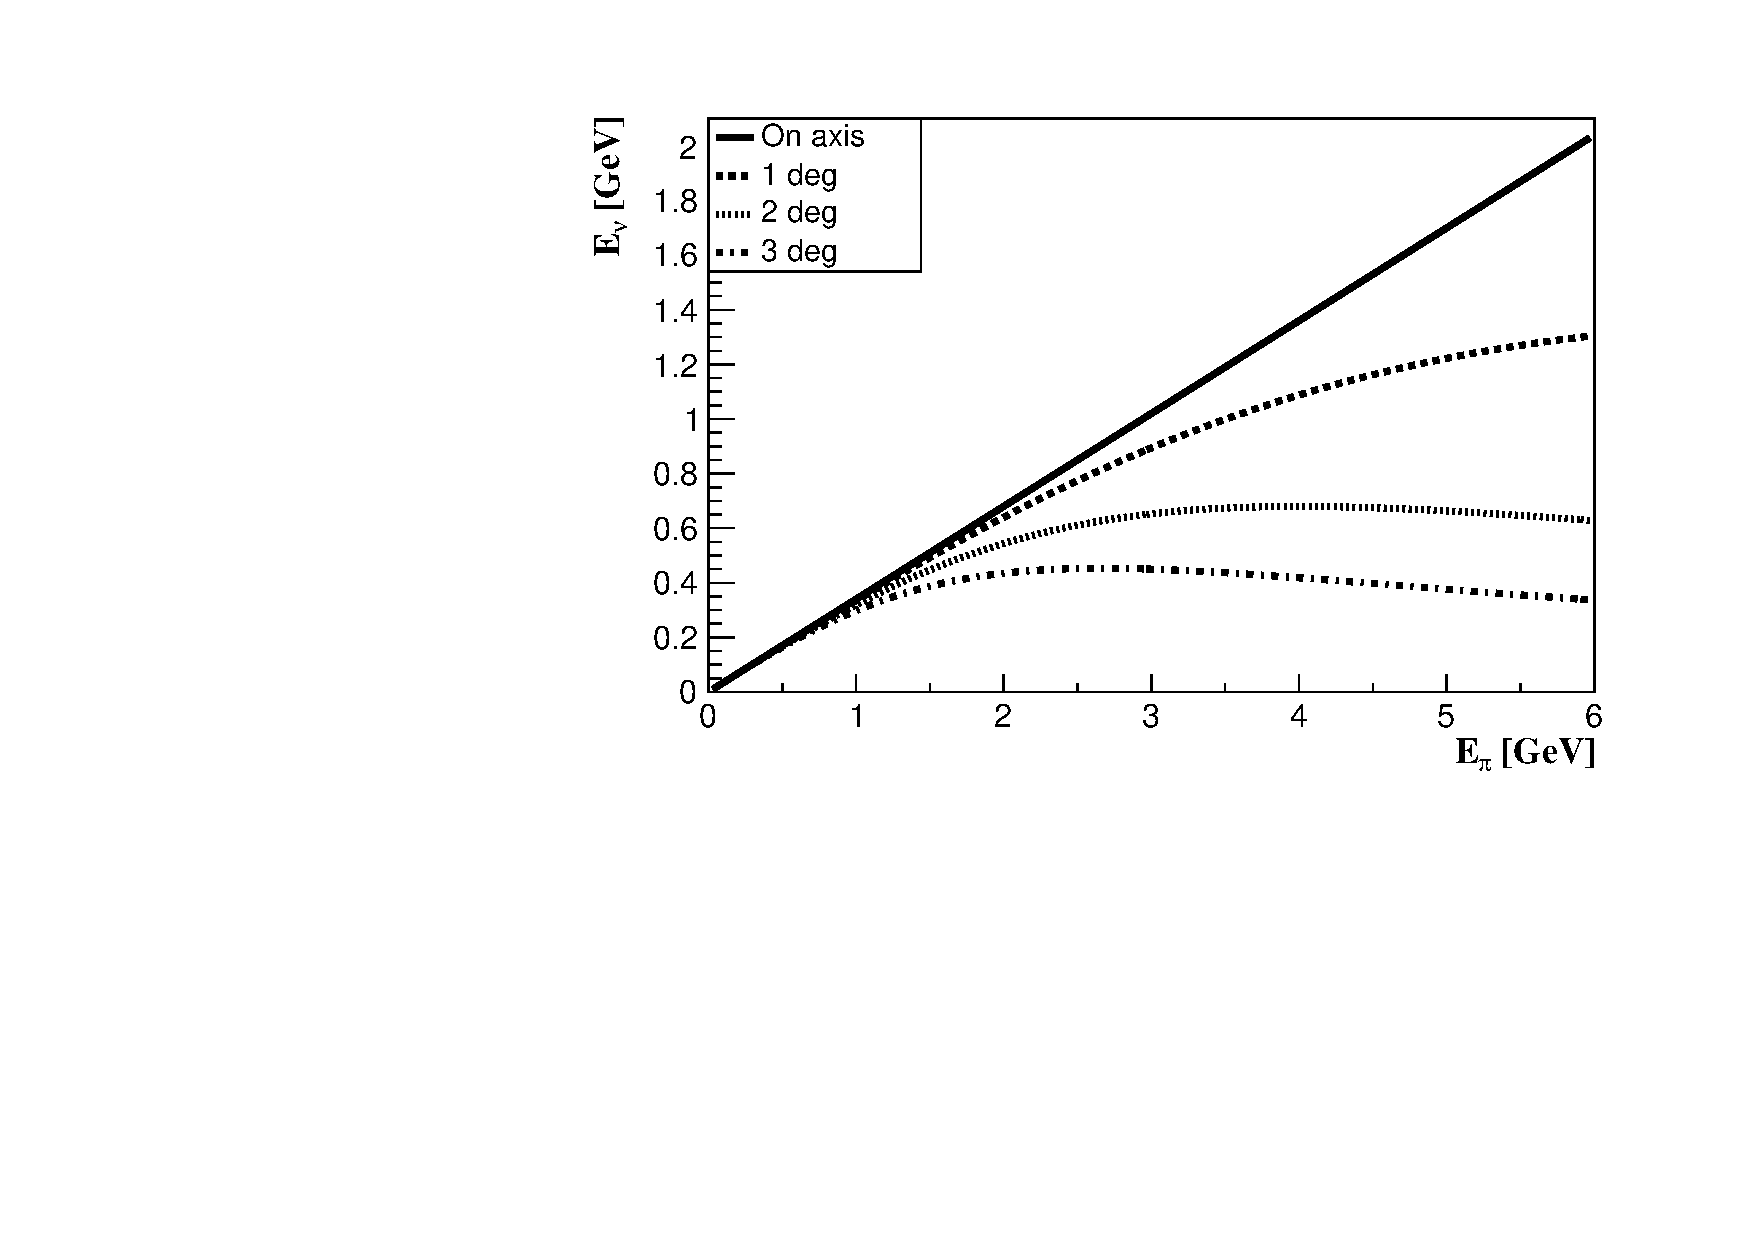
\includegraphics[width=0.6\linewidth]{figures/offaxis.pdf}
  \caption{Neutrino energy as a function of the pion energy for on-axis decays and several off-axis angles. For a non-zero off-axis angle, the neutrino energy reaches a maximum. This feature is currently exploited in the T2K and \nova experiments.}
 \label{fig:offaxis}
 \end{figure}


As the neutrino beam is a tertiary beam, it is necessary to include in the experimental apparatus monitoring devices to ensure that it is stable in intensity and direction. To this effect, muon detectors, sensitive to the muons produced by the pion decays, are placed close to the end of the decay volume. Moreover, as the neutrino flux and cross-sections and the beam composition are not known with sufficient precision, a near detector is located close to the target station (typically within a few hundred meters). The near detector constrains the neutrino interaction rate, proportional to the product of the neutrino flux and the cross-section. Moreover, the near detector allows to measure the beam composition and to perform study of several neutrino cross-section.    

For recent long baseline experiments it is especially important that the beam is very pure in $\nu_\mu$. An irreducible $\nu_e$ component, at the percent level, is always present, due to the decay of muons, produced by the decay of pions. Another source of $\nu_e$ is due to the K$_{e3}$ semileptonic decay of kaons.

In the antineutrino mode, the fraction of neutrinos in the beam is relatively large (for instance xx\% in the T2K antineutrino beam) due to the fact that the $\pi^+$ cross-section is higher than the $\pi^-$ cross-section. These impurities in the beam need to be measured, for instance with a magnetized near detector. 

\begin{table}
\centering
\begin{tabular}{|c|c|c|c|c|c|}
  \hline
  Exp. & Energy (GeV) & Power (kW) & L (km) & FD mass (kt) & POT \\ 
  \hline
K2K & 30 & & 250 & 22.5 & 9.2 10$^{19}$\\
MINOS & 120 & 700 & 790 & 5.4 & 8.2 10$^{20}$\\
OPERA & 450 & 400 (?) & 730 & 1.8 & 1.8 10$^{20}$\\
T2K & 30 & 750 & 295 & 22.5 & 8 10$^{21}$\\
\nova & 120 & 700& 810 & 14 & \\
HK & 30 & 1300 & 295 & 380 & \\
DUNE & 120 & 1200 & 1300 & 40 &\\
  \hline
\end{tabular}
\caption{Parameters of recent and future long baseline experiments. Energy and power refer to the primary proton beam, L is the baseline, FD the mass of the far detector. POT (Proton On Target) represents the integrated dataset as of 2016 for the running experiments, the total foreseen exposure for future projects.}
\end{table}

\subsection{Flux and cross-section systematic uncertainties}
\label{sec:beamsyst}

The measurement of neutrino oscillations has now reached the precision era. Particularly long-baseline neutrino oscillation experiments require a good control of the systematic uncertainties related to neutrino fluxes and neutrino cross-sections to perform measurements of oscillation parameters. 

A common strategy to reduce systematic uncertainties, used in most of the long baseline experiments, is the use of a Near Detector complex, located at few hundreds of meters from the beam target. In this way the neutrino spectrum and the flavor composition of the beam can be precisely measured before the oscillations and this is used to determine the expected spectra at the far detector.

Some long-baseline experiments, as for example MINOS and \nova, uses as near detector a detector that has the same composition as the far detector so that cross-section uncertainties due to the different target nuclei or detector systematic uncertainties are minimized in the extrapolation. Other experiments, as for example K2K and T2K, uses a set of near detector, with different target nuclei, in order to maximize the information on the cross-section models.

In this section, as an example, we will briefly describe how the T2K experiment uses the near detector data to reduce the systematic uncertainties in the oscillation analysis. The T2K near detector, called ND280, is magnetized, with several sub-detectors installed within the ex UA1/NOMAD magnet that provides a 0.2 T magnetic field. For the oscillation analysis the ND280 tracker system is used, comprising two Fine Grained Detectors (FGD) interleaved with three Time Projection Chambers (TPC). The FGDs act as an active target for neutrino interactions (each with a mass of 2~ton). Particles produced in the FGD enter the TPCs where the charge and the momentum of the tracks is reconstructed as well as the particle identification based on the measurement of the energy loss in the gas. One important point to notice is that one of the two FGD is a fully active detector while in the second one scintillator layers are interleaved with inactive water layers, allowing to select neutrino interactions on carbon and on oxygen, the same target as the far detector, SK. 
    
At T2K energies most of the \num charged current neutrino interactions are quasi-eleastic events, producing only one visible track in the final state, the muon. The proton has often a low momentum around 200 MeV/c, its track too short to be reconstructed. The presence of the magnetic field allows to reconstruct the charge of the muon, distinguishing between negative muons produced by \num and positive leptons produced by \numb interactions.
In some cases neutrinos exchange enough energy with the target nuclei producing also pions or protons that can, in some cases, enter the TPC. 
For \num selections, ND280 distinguishes three cases on the basis of the final state topology: only the muon is reconstructed (CC0$\pi$, with a xx \% purity of CCQE events), the muon and one negative pion is also reconstructed (CC1$\pi$) and events with more pions (CCother, essentially deep-inelastic events). For \numb selections interaction with one track are separated from the interactions with more than one track.
  
The same selections are applied to interactions in both the FGD and all the samples are then fit to reduce systematic uncertainties on the flux and cross-section model. 
The main uncertainty on the flux model is due to the hadron production cross-section. Data from the NA61/SHINE experiment at CERN are used. In NA61/SHINE a proton beam is accelerated to 30 GeV/c and strikes a target. Hadrons produced are measured with a system of TPCs and Time Of Flight detectors, and double differential cross-section (in angle and momentum) are extracted. Thanks to NA61/SHINE data the uncertainties on the neutrino fluxes, prior to the ND280 fits, are reduced to the 10-15\% level.

For the cross-section model, the priors are based, as much as possible, on external experiments such as MiniBooNE and MINERvA. An important aspect is that, for the first time, effects related to the multi-nucleon 2p-2h emissions are included in this analysis, based on the Nieves model~\cite{Nieves:2011yp}

To reduce flux and cross-section uncertainties, the ND280 samples are binned in the kinematic variables \ptheta according to the muon momentum and angle with respect to the beam direction. Data and Monte Carlo are fitted using a binned likelihood, where the prediction for each bin depends on the flux, cross-section and detector systematic parameters. 

The result of the fit is a set of point estimates and covariance for the systematic scaling factors for the unoscillated neutrino flux at SK. The impact of the ND280 fit on the total error budget in the T2K oscillation analysis is shown in Tab.~\ref{tab:t2ksyst}: a reduction of the systematic uncertainties from $\sim15\%$ to $\sim5\%$ is obtained thanks to the near detector fit.

In the case of \nova, they profit of the fact that the near and the far detector are identical and use a calorimetric approach in which all the energy observed in the event at the near detector is reconstructed and is then unfolded to obtain the expected true neutrino energy. The far to near ratio and the oscillation probabilities are then applied to obtain the expected true energy spectrum at the far detector. This method allow to reduce the total systematic uncertainty to level similar to the ones obtained by T2K.

\subsection{Results from long-baseline accelerator experiments}

K2K (KEK-to-Kamioka) was the first long baseline neutrino beam, using Super-Kamiokande as its far detector at 290 km from the neutrino production. Operating between 1999 and 2004, it has measured the disappearance of $\nu_\mu$: 112 events were observed, while 158.1$^{+9.2}_{-8.6}$ were expected without oscillation, a 4.3 $\sigma$ effect~\cite{Ahn:2006zza}. This measurement has confirmed neutrino oscillation as the explanation for the atmospheric neutrino disappearance. 

Further precision measurements of the $\nu_\mu \rightarrow \nu_\mu$ were reported by MINOS, T2K and NOvA. In particular, T2K and \nova use a narrow band beam, based on the off-axis design, that is particularly suited for the measurement of \num disappearance once the mass square difference is known. For a given \dmsq and a given baseline distance, in fact, the oscillation probability depends on the neutrino energy that can be tuned by changing the off-axis angle. In the case of T2K (L=295~km) the maximum of the oscillation is at an energy of 600 \mev while in the case of \nova  (L=810~km) the maximum is at 1800 \mev. 

While the most recent analyses published by T2K do a global fit of appearance and disappearance modes to extract the maximum of the information on neutrino oscillations in the PMNS framework, disappearance analyses only have also been done by T2K in order to test the PMNS framework. In the \num disappearance probability in fact there are no CP odd terms so the disappearance probability is expected to be the same for \num and \numb. Previous results from MINOS showed some tensions between neutrinos and antineutrinos. 

For the T2K experiments, fully contained \num events are selected in Super-Kamiokande in time with the beam, with one ring identified as produced by a muon and less than two decay electrons. The resulting sample is composed by 62 \% of CCQE $\nu_\mu$ events, 32 \% of non-CCQE $\nu_\mu$ events and the rest essentially by NC events.
Based on \nupot protons-on-target (POT) collected in neutrino mode and \nubpot POT collected in antineutrino mode, T2K has observed 135 (66) \num (\numb) candidates at SK with 522 (185) events expected in case of no-oscillations and 135.8 (64.2) events expected for maximum disappearance. The reconstructed energy spectrum for both, \num and \numb surviving events are shown in Fig.~\ref{fig:t2kdis}. Thanks to the use of the Near Detector data described in Sect.~\ref{sec:beamsyst}, the systematic uncertainties on these measurements are smaller than 5\% and a precise measurement of \thatm and \dmsq is obtained as shown in Fig.~\ref{fig:atm-contour}. The oscillation parameters measured are in excellent agreement between neutrinos and antineutrinos and both are compatible with maximal mixing for \thatm.

\begin{figure}[htbp]
\centering
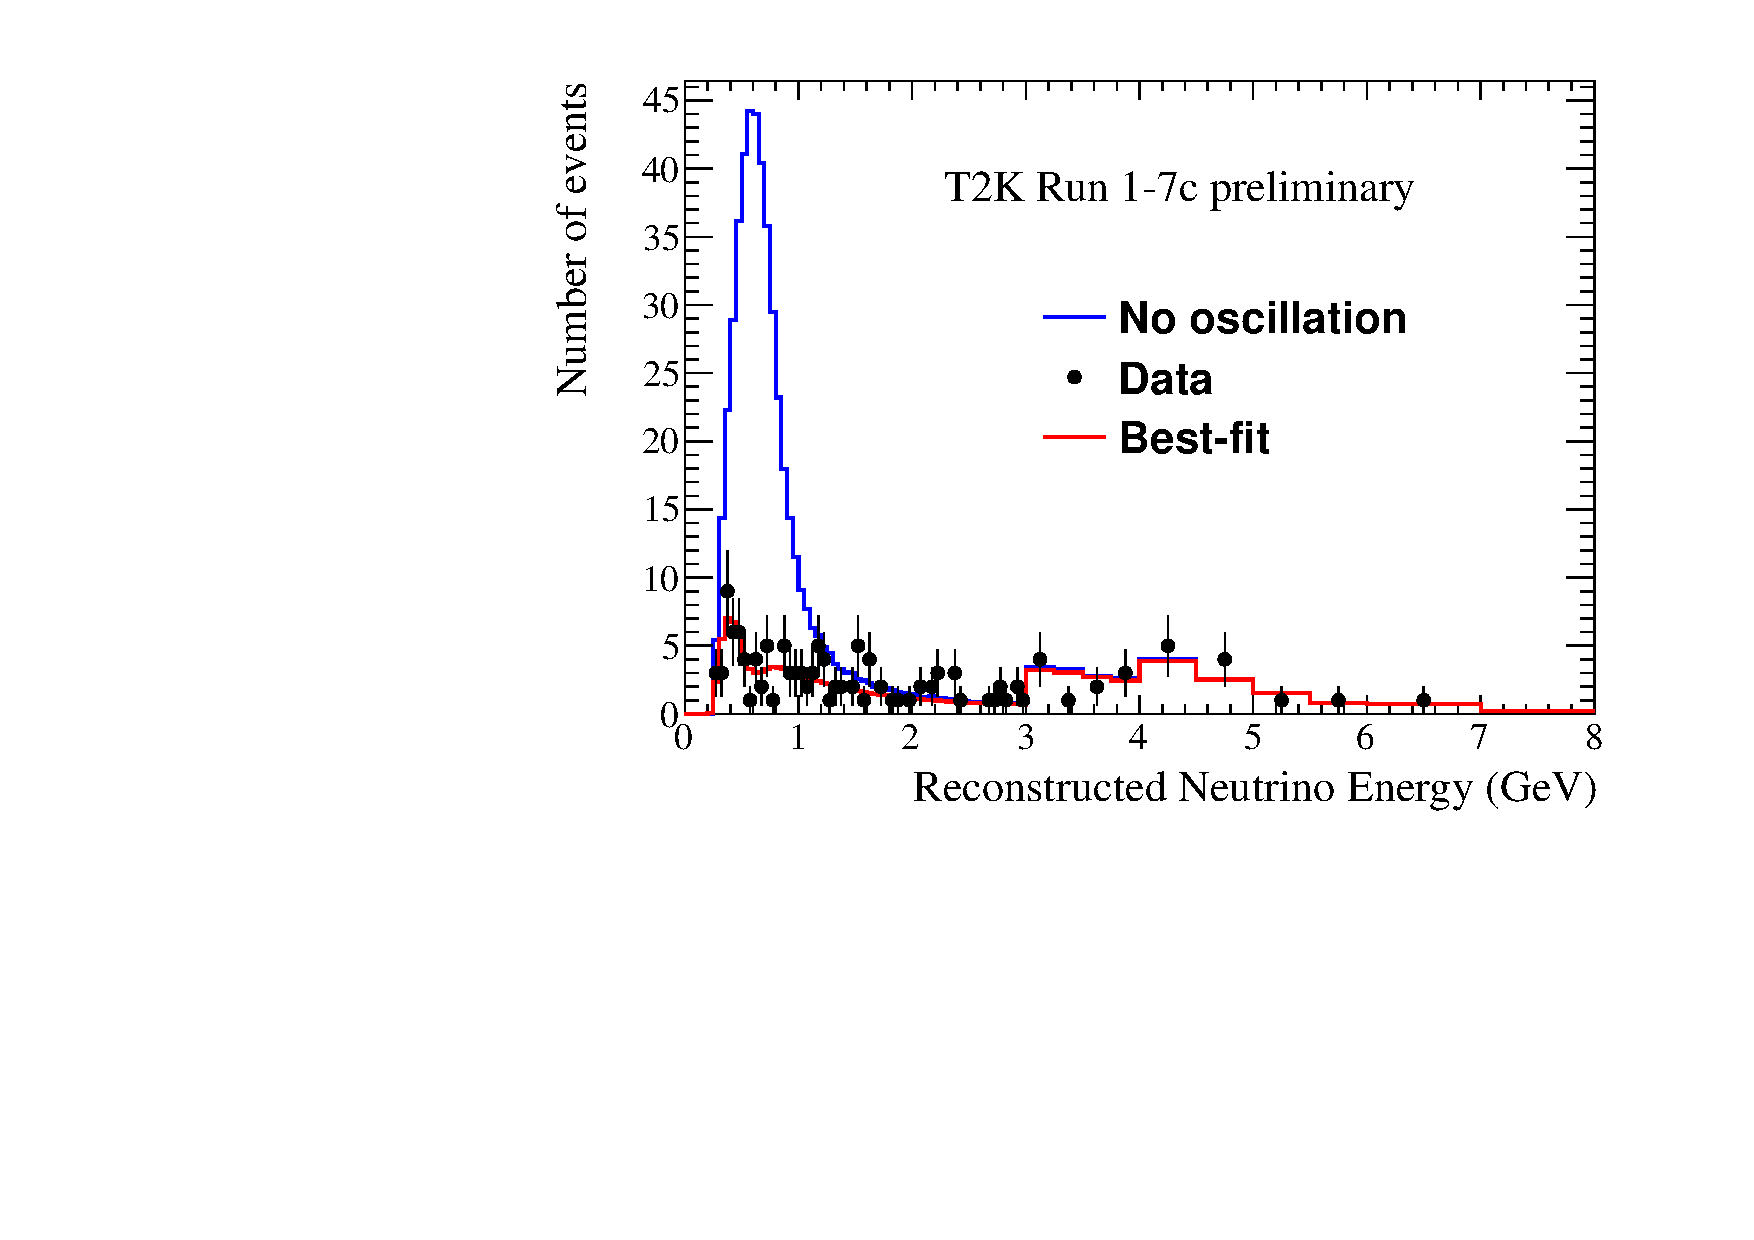
\includegraphics[width=0.4\linewidth]{figures/bestfit_sinsqth23vsdcpvsmh_1rmu_run17.pdf}
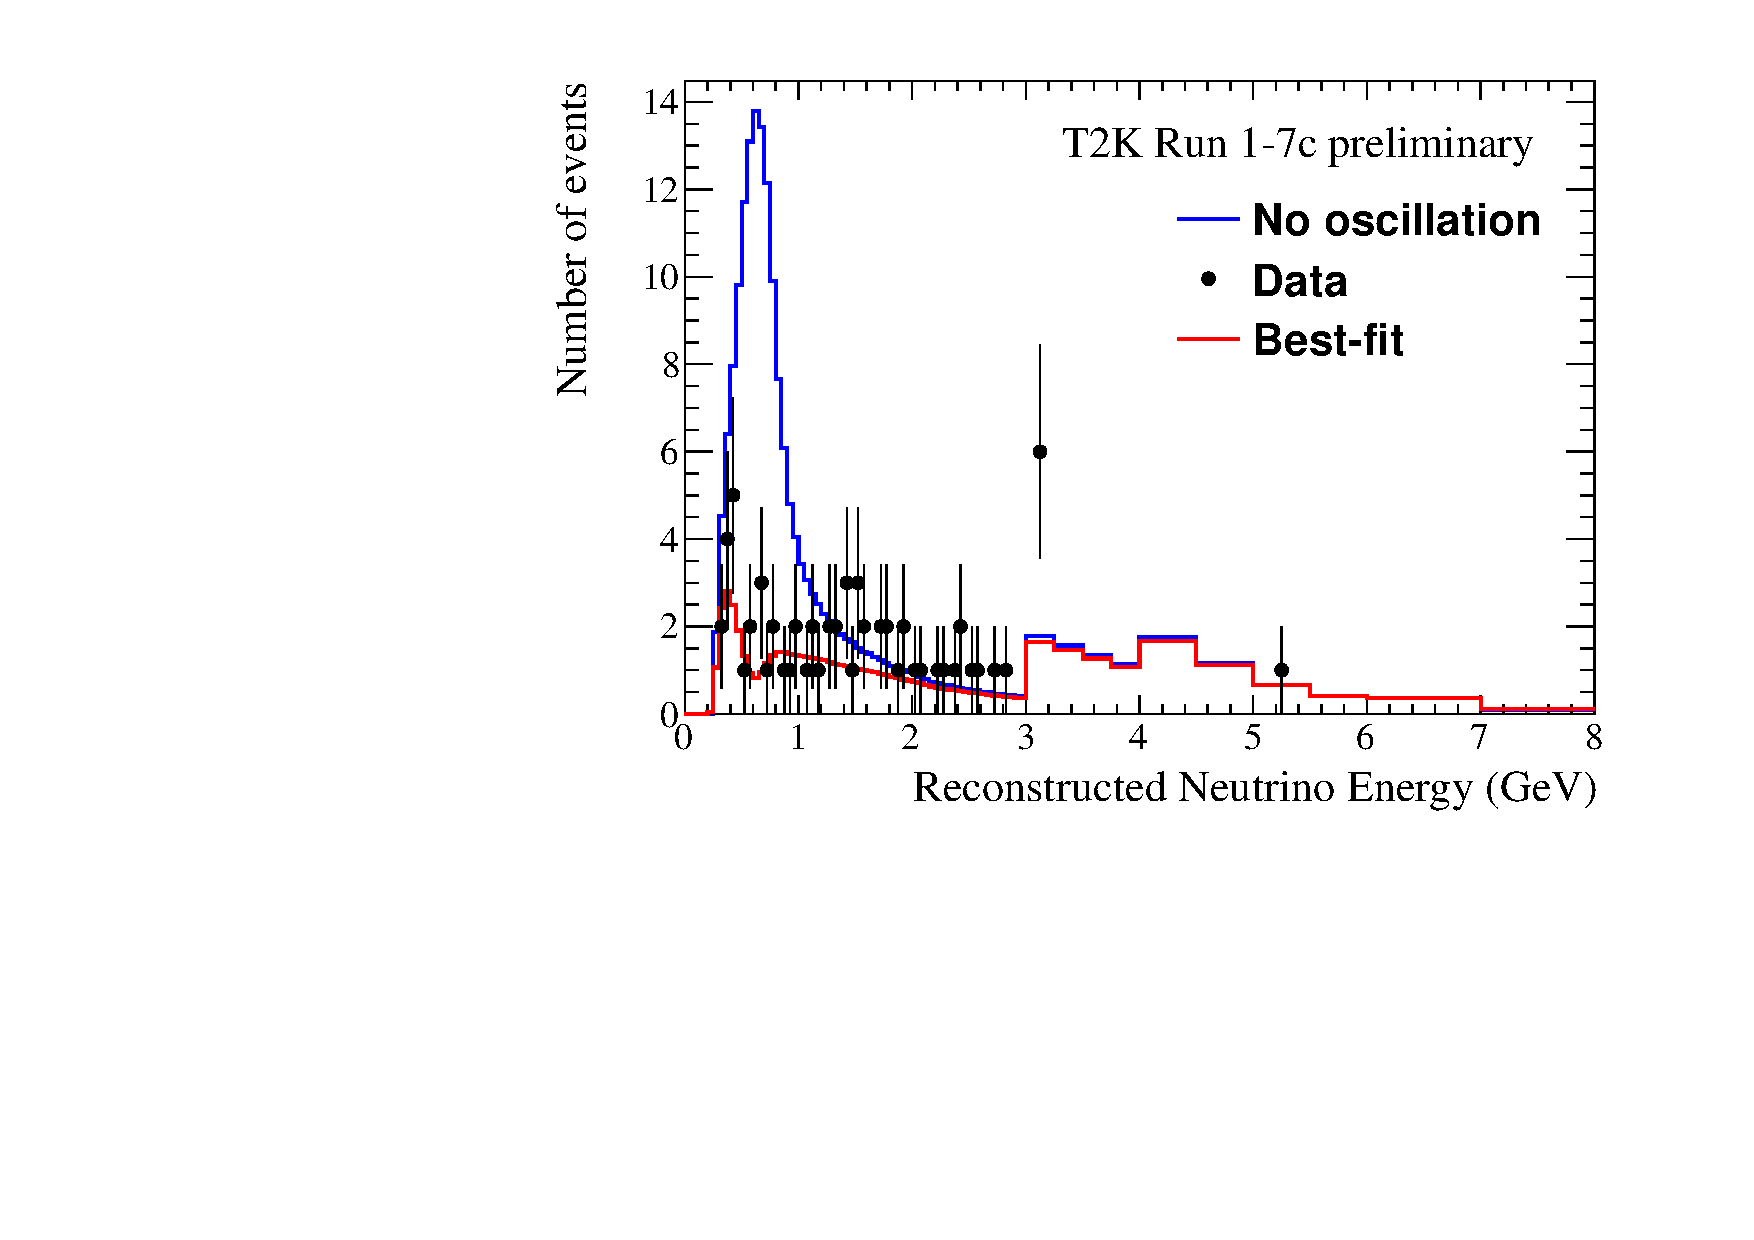
\includegraphics[width=0.4\linewidth]{figures/bestfit_sinsqth23vsdcpvsmh_rhc1rmu_run17.pdf}
  \caption{
Reconstructed \num and \numb energy spectrum by the T2K collaboration for data, best-fit prediction, and
unoscillated prediction. %Bottom: Ratio of oscillated to unoscillated events as a function of
%neutrino energy for the data and the best-fit spectrum.
}
 \label{fig:t2kdis}
 \end{figure}

\begin{figure}[htbp]
\centering
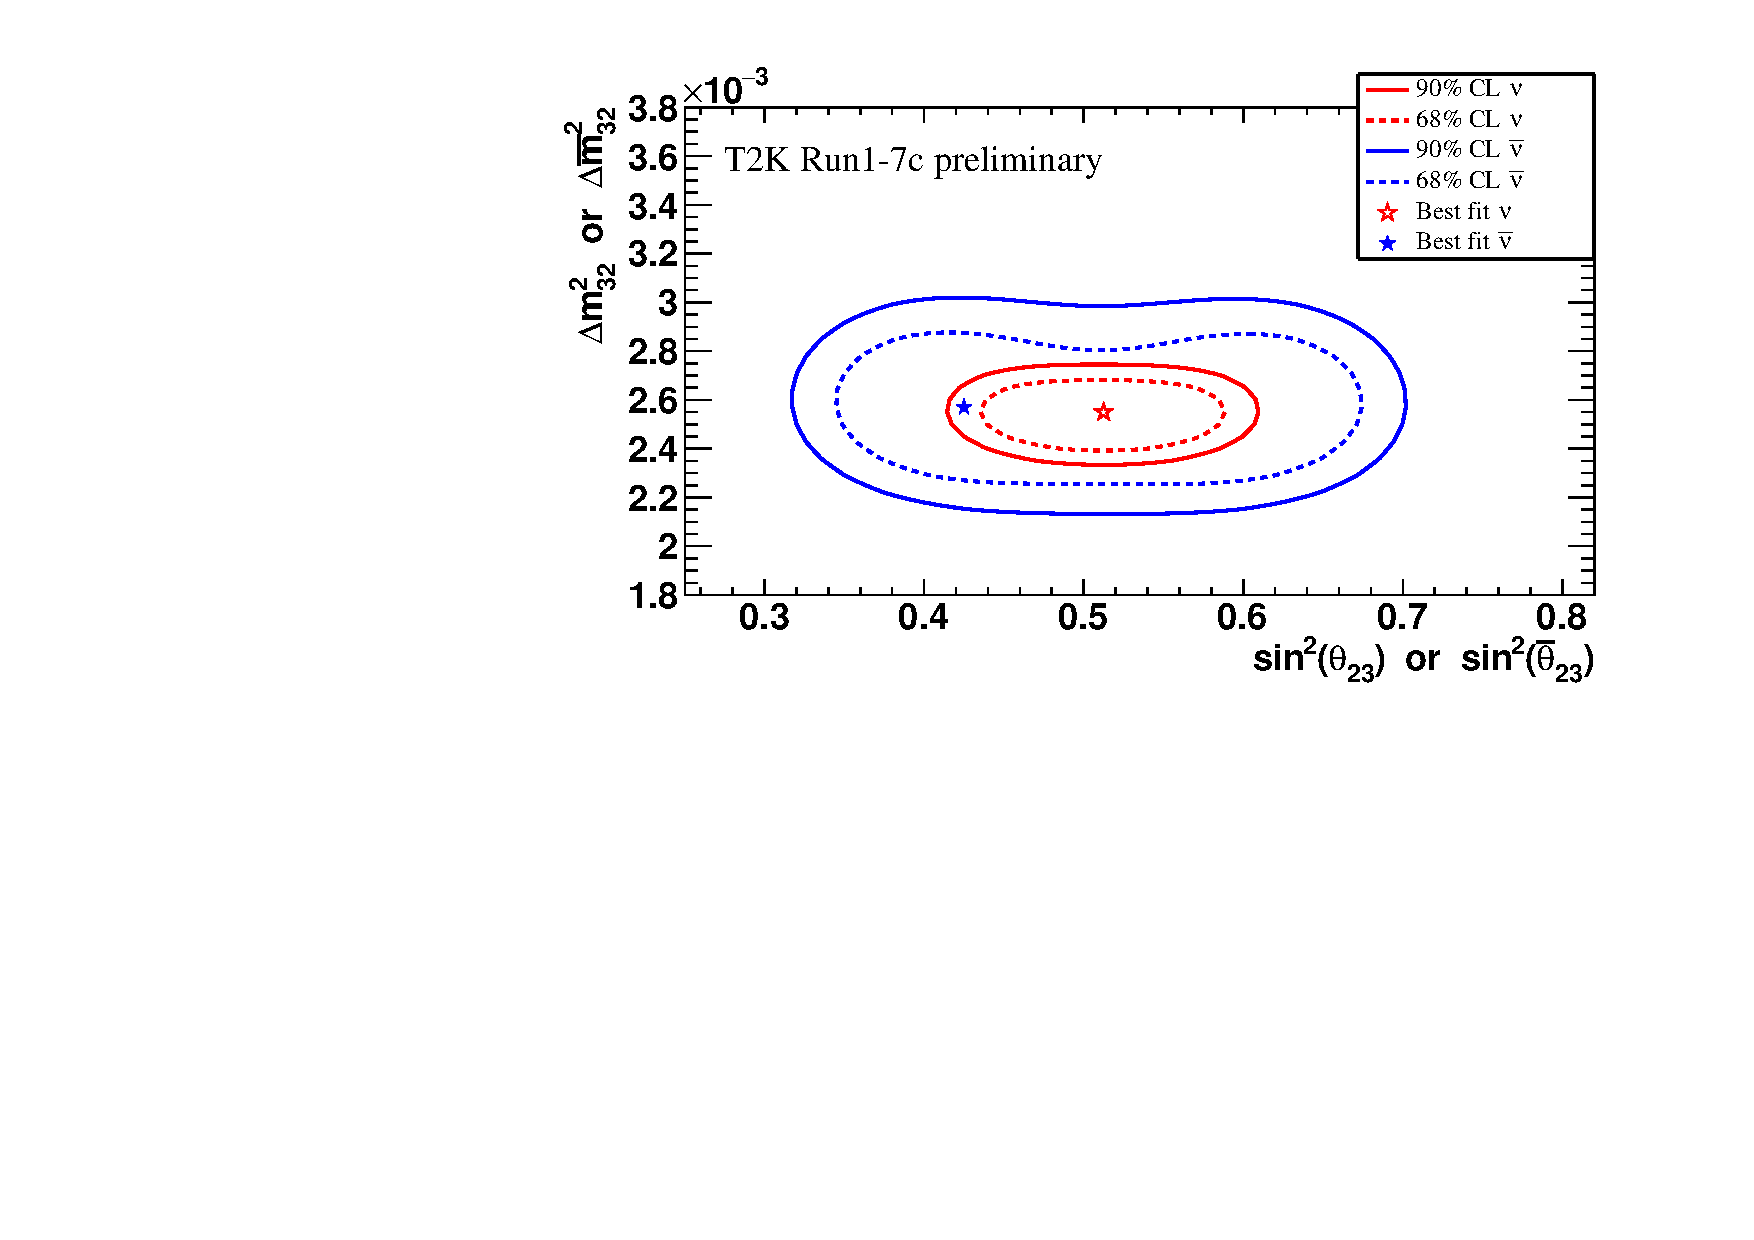
\includegraphics[width=0.6\linewidth]{figures/nu_vs_nubar_datafit_17c_nh.pdf}
  \caption{$\Delta m^2 $ versus \stt for neutrinos and antineutrinos parameters. The constant $\Delta \chi^2$ critical values in the gaussian approximation are shown.}
 \label{fig:atm-nunubar}
 \end{figure}

\nova has also reported a measurement of \num disappearance using \novapot POT and by selecting \mmu-like candidates at the far detector. They observed 78 events in the far detector, while $473\pm30$ were expected without oscillations. This result lead to some tensions, especially with the T2K experiment, since maximal mixing is excluded by NOvA at $2.5\sigma$ as shown in Fig.~\ref{fig:atm-contour}. 

\begin{figure}[htbp]
\centering
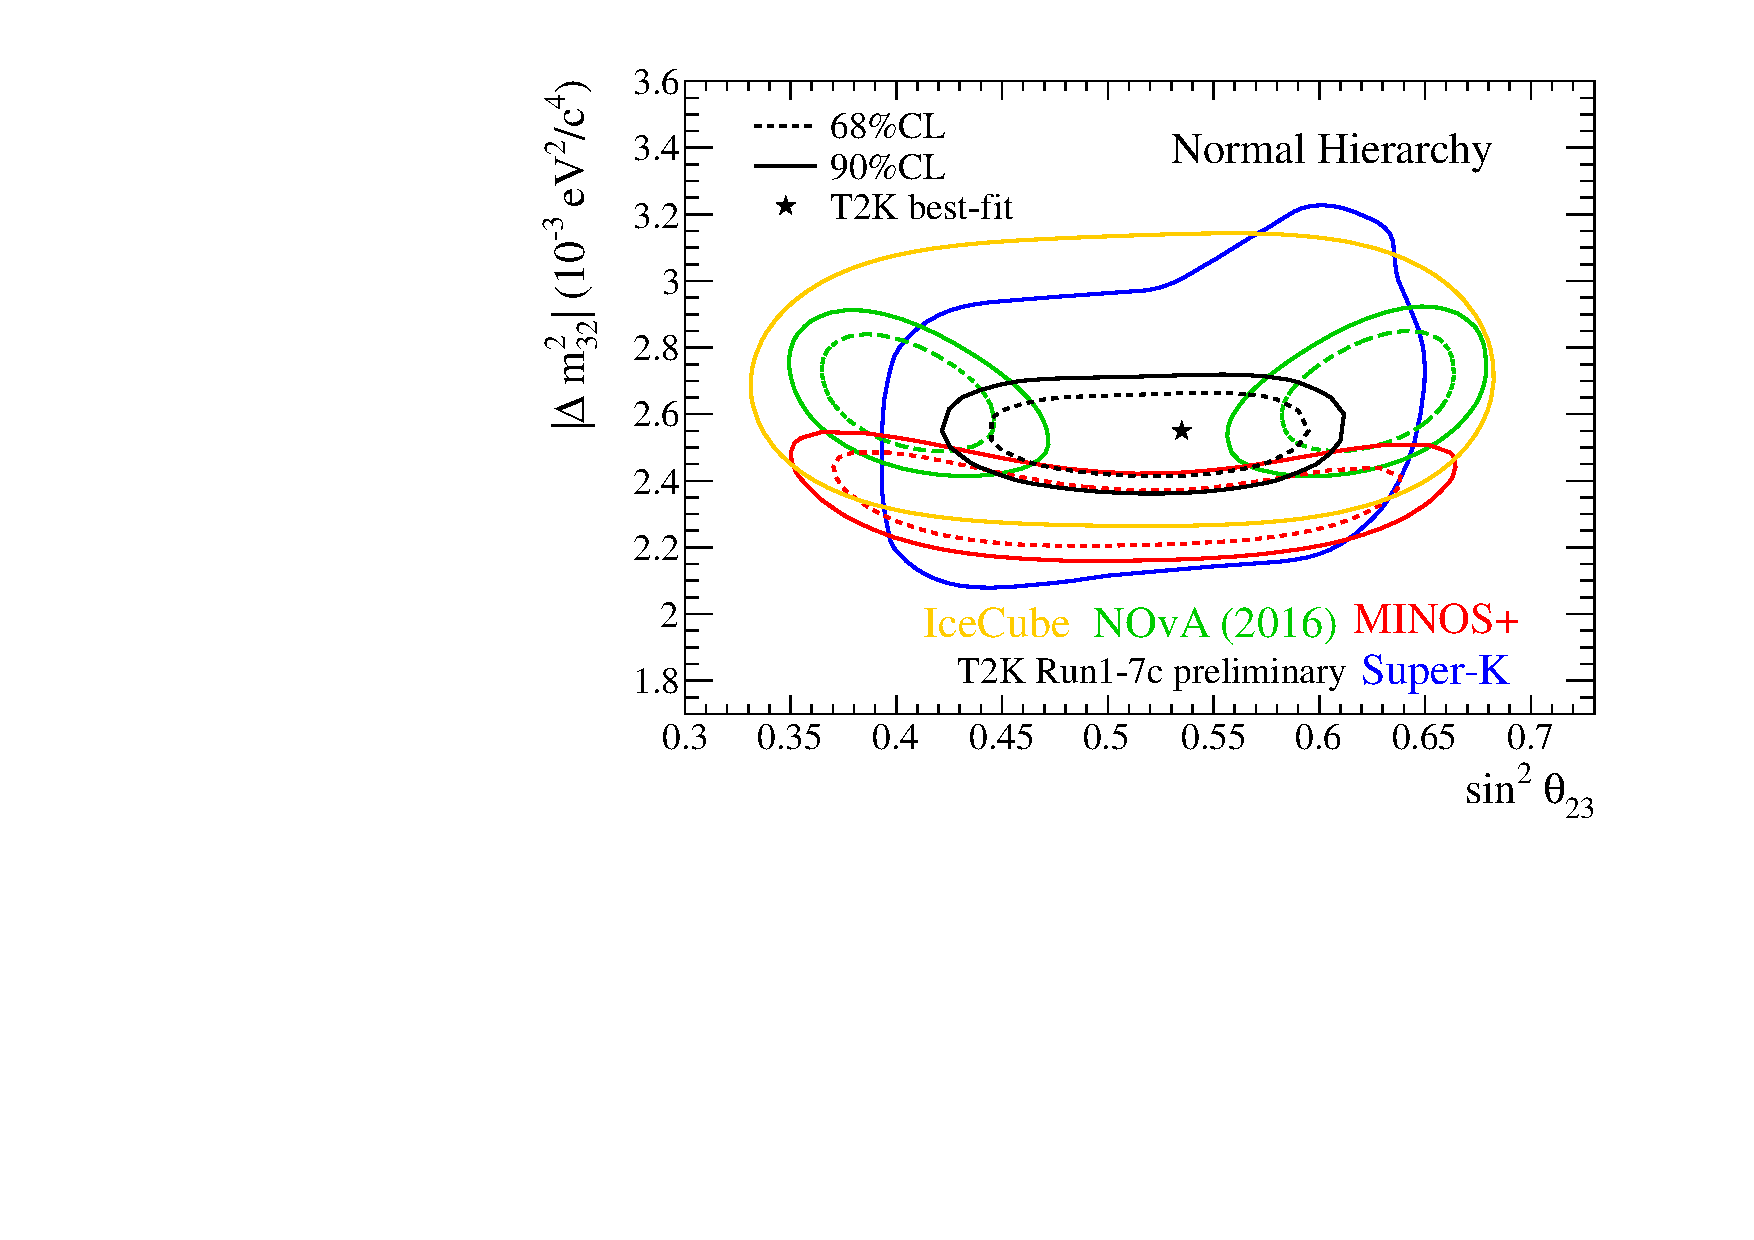
\includegraphics[width=0.5\linewidth]{figures/sinsqth23vsdmsq_react_othexp_nh.pdf}
%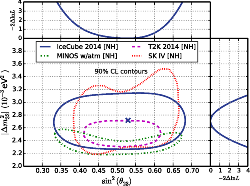
\includegraphics[width=0.6\linewidth]{figures/atm-contour.pdf}
  \caption{
Measured $\Delta \chi^2$ distributions as a function of $\sin^2 \theta_{23}$, $\Delta m^2_{32} (\Delta m^2_{13})$ for T2K, Super-K (PoS ICRC2015 (2015) 1062), Minos+ (Neutrino 2014 conference), \nova (Phys.Rev. D93 (2016) 051104, arXiv 1601.05037) and IceCube DeepCore (Phys.Rev. D91 (2015) 072004, arXiv 1410.7227).}
 \label{fig:atm-contour}
 \end{figure}
 
The two collaborations are working to understand this difference that could still be simply due to statistical fluctuations. A comparison between reconstructed energy spectrum for the best-fit and the one obtained by imposing maximal mixing in \nova is shown in Fig.~\ref{fig:novadiscomparison}. Something similar is done by T2K comparing their data, the T2K best fit and the spectrum obtained by imposing the NOvA best-fit oscillation parameters as shown in Fig.~\ref{fig:t2kdiscomparison}. Additional data from both, T2K and NOvA will help to clarify the situation. 
 
 \begin{figure}[htbp]
\centering
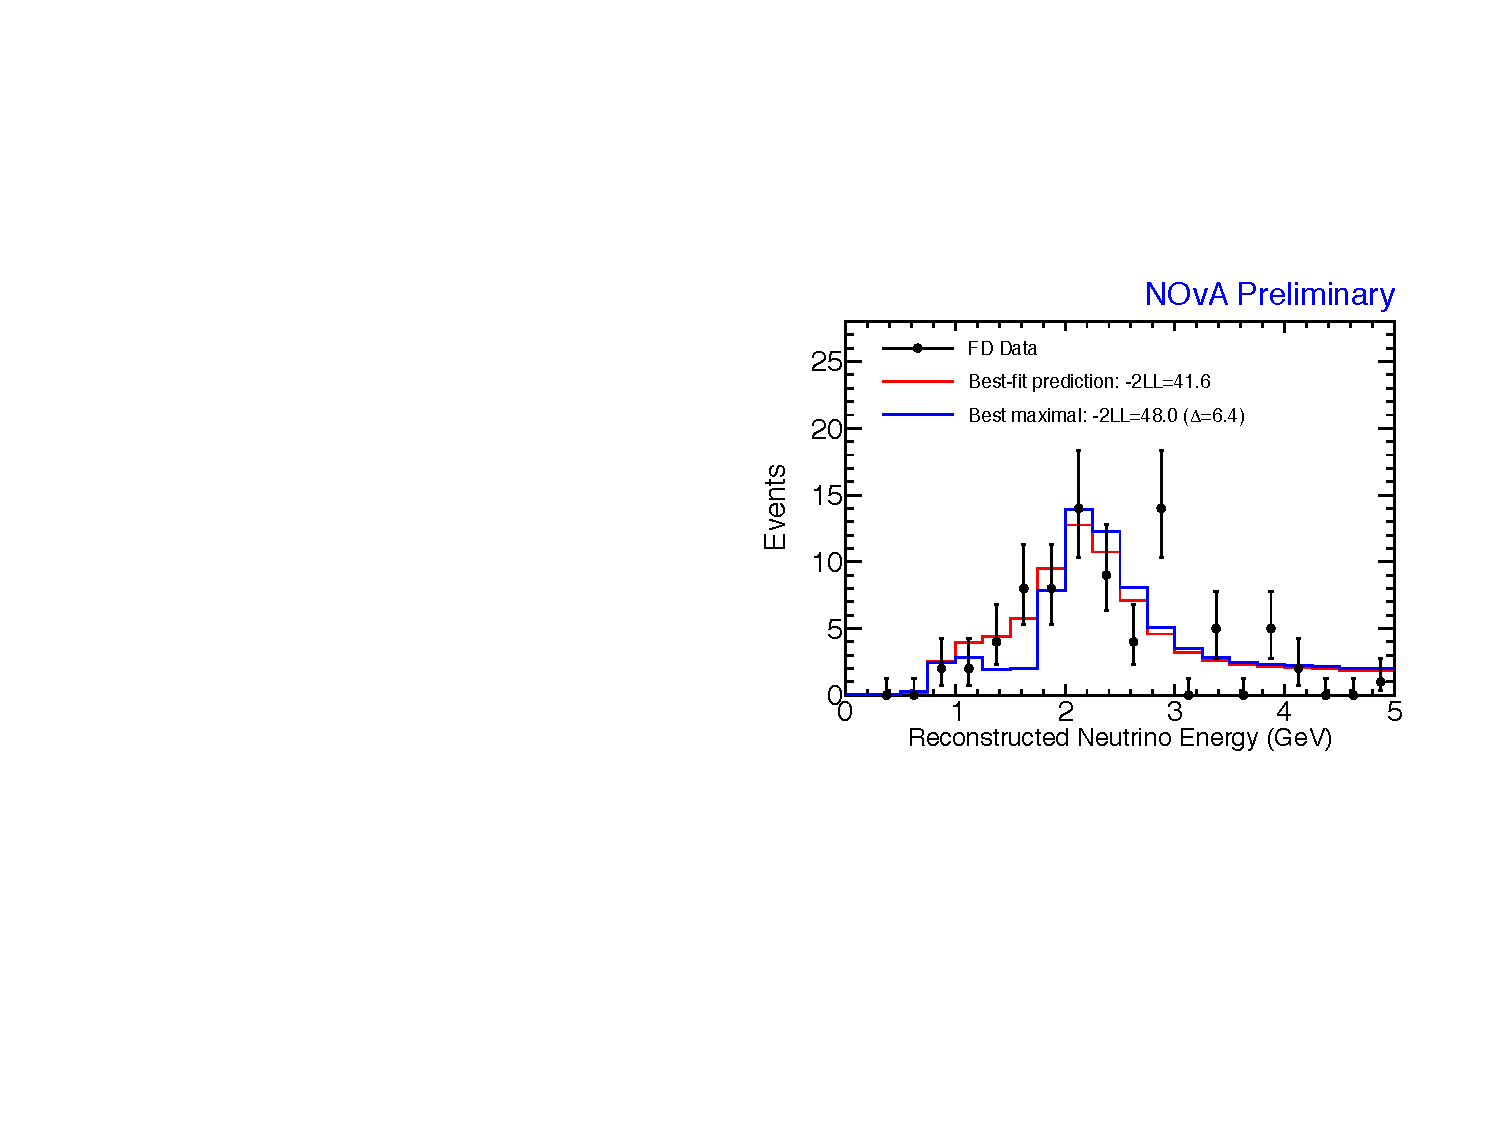
\includegraphics[width=0.6\linewidth]{figures/nova_comparison.pdf}
  \caption{Reconstructed energy spectrum in \nova for data, best fit and best fit assuming maximum mixing} \label{fig:atm-nova}
 \end{figure}
  
 
 \subsection{Evidence for $\nu_\tau$ appearance}

The OPERA experiment on the CERN to Gran Sasso neutrino beam, taking data between 2008 and 2012, was designed to test the $\nu_\mu \rightarrow \nu_\tau$ appearance hypothesis. The detector is based on the Emulsion Cloud Chamber technique, with 1800 ton of nuclear emulsion detectors in the forms of bricks, each brick being composed of a stack of nuclear emulsion film and lead plates. This target, capable of sub-micrometric track resolution, is devoted to the study of the neutrino interaction vertex and the particles associated to it. The identification of the $\tau$ leptons relies mainly on their characteristic kink (Fig.~\ref{fig:opera}) due to the decay $\tau \rightarrow h \nu_\tau$, or $\tau \rightarrow l \nu_\tau \bar \nu_l$, where $h$ is a charged meson, and $l$ is an electron or a muon. Another signature is related to the decay $\tau \rightarrow 3 h \nu_\tau$ where the short $\tau$ track ends in a three-pronged vertex. The target detectors are complemented by scintillator trackers and muon spectrometers. 

OPERA has observed 5 $\nu_\tau$ candidate events \cite{Agafonova:2015jxn} with a total background of 
$0.25 \pm 0.05$ events, mainly coming from decays of charmed particles. This corresponds to a 5.1 $\sigma$ observation of $\nu_\tau$ production in an oscillated $\nu_\mu$ beam. 

The Super-Kamiokande collaboration has also searched for $\nu_\tau$ appearance in multi-ring events to test the hypothesis of $\nu_\mu \rightarrow \nu_\tau$ oscillations~\cite{Abe:2012jj}. While the selected sample is affected by large backgrounds, there is an excess of tau-like events in the upward-going direction with a significance of 3.8 $\sigma$, offering a complementary confirmation of the OPERA result.  
 
\begin{figure}[htbp]
\centering
%\includegraphics[width=0.5\linewidth]{energy_miniboone.eps}
%\includegraphics[width=0.6\linewidth]{figures/topology_modified.pdf}
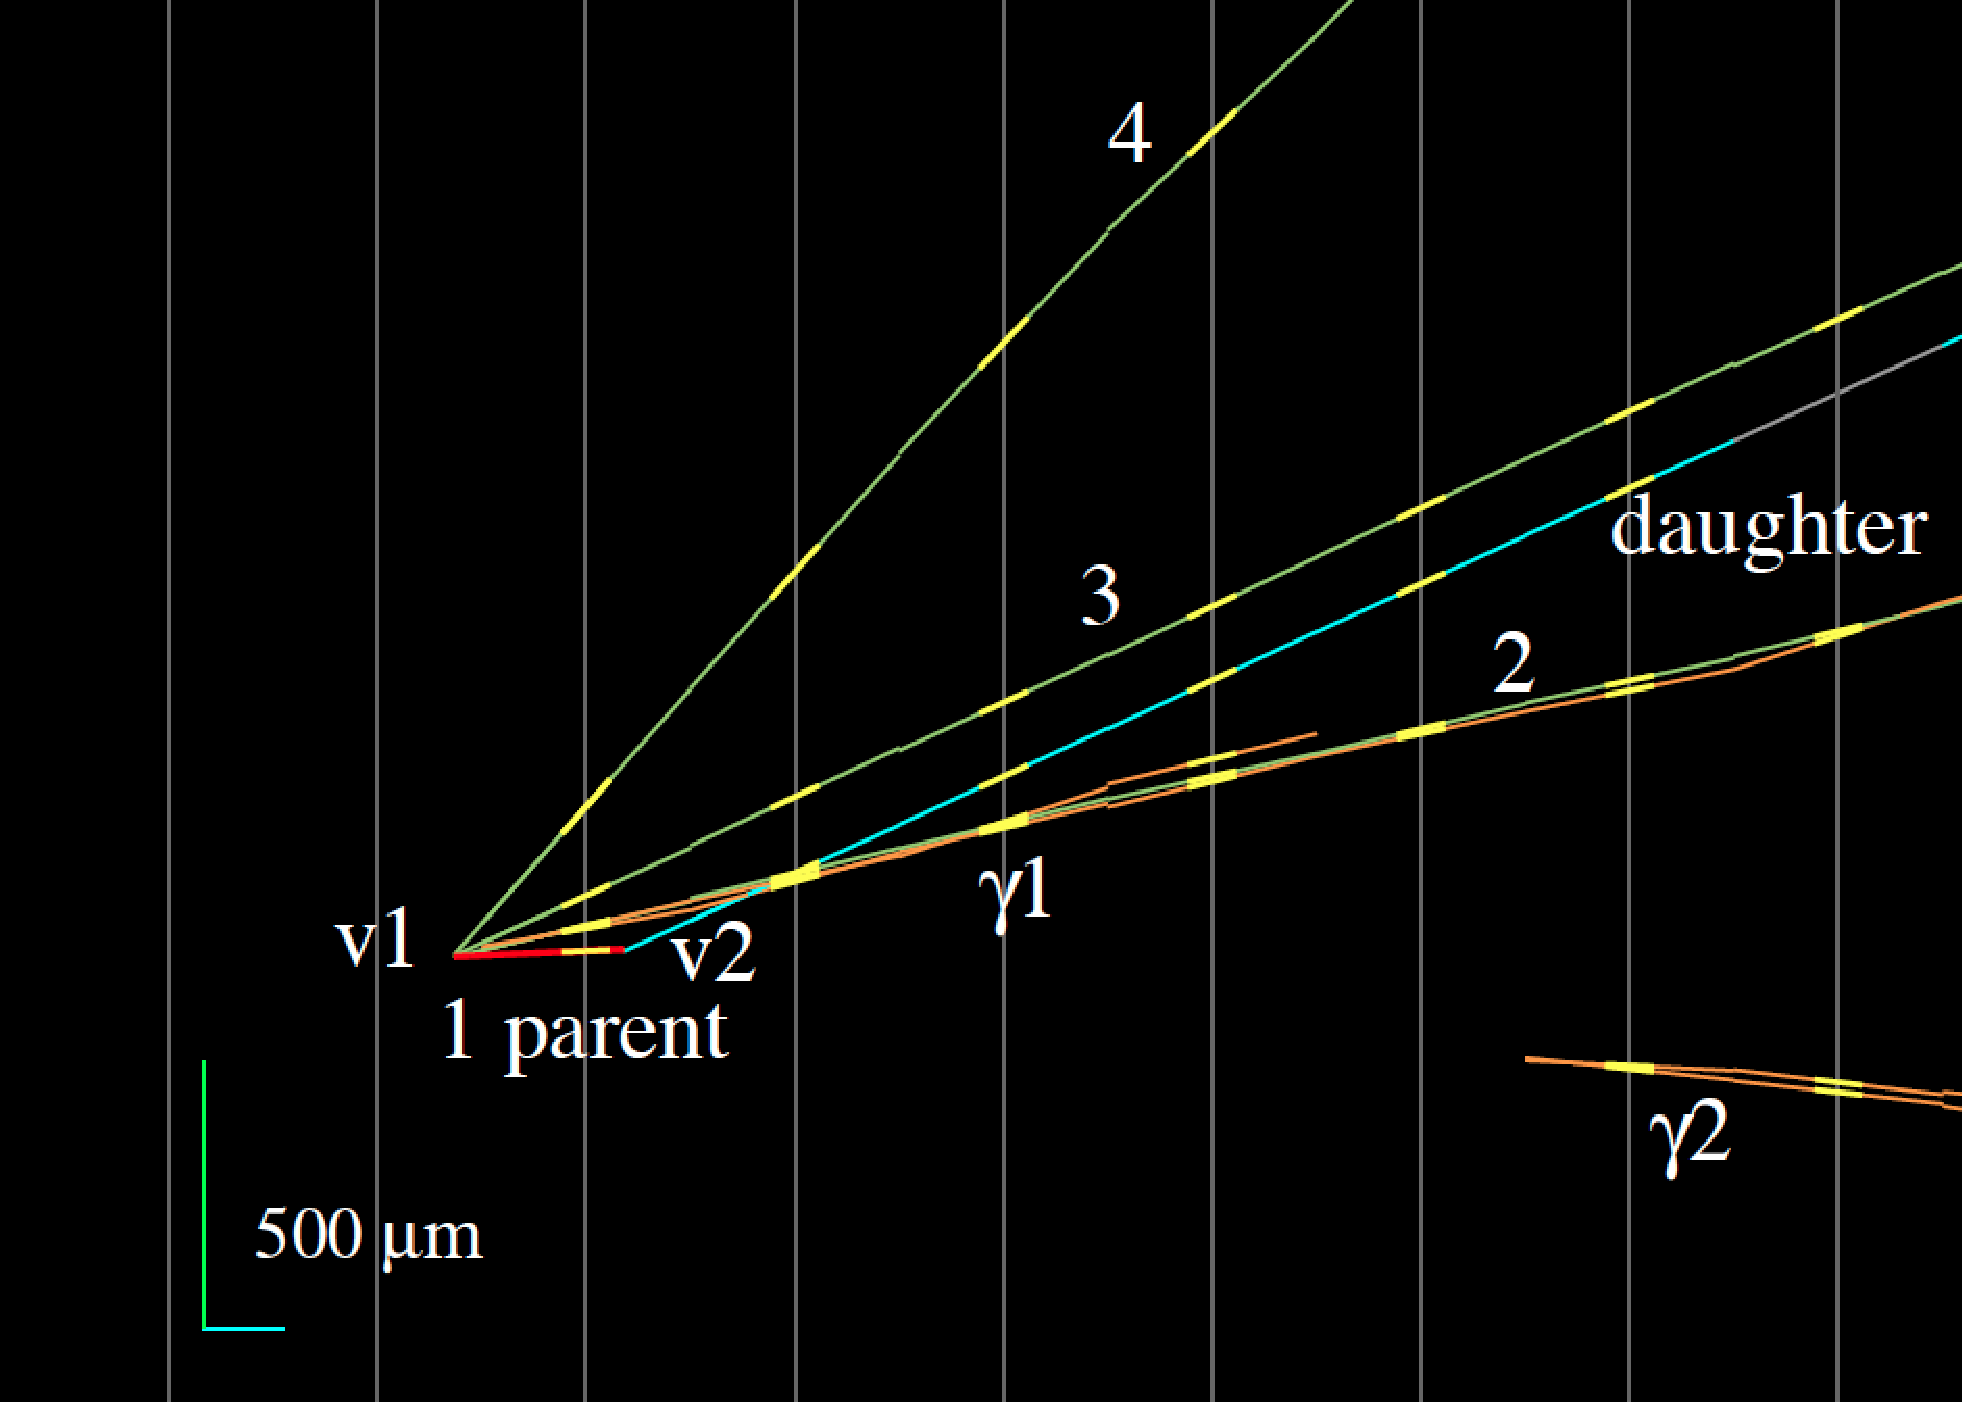
\includegraphics[width=0.6\linewidth]{figures/tau4.pdf}
  \caption{
Event display of the fourth $\nu_\tau$ candidate event from the OPERA 
experiment~\cite{DICRESCENZO2015186} in the
horizontal projection longitudinal to the neutrino direction.
The primary and secondary vertices are indicated as V$_0$ and
V$_1$ , respectively. The kink between the parent and daughter track, a feature of $\tau$ lepton decays, is clearly visible. The yellow stubs represent the track segments as measured in the emulsion films.  
}
 \label{fig:opera}
 \end{figure}



\clearpage
%% Strategy to measure th13
%\subsection{The 1-3 sector (MZ)}


Solar and atmospheric results are well described by two-flavour mixing models, but we know that there are at least three neutrino flavours and therefore at least three mass eigenstates. The experiments described so-far, while giving robust evidence for neutrino oscillation, do not provide a full picture of 3x3 mixing models. 

In order to fully establish the PMNS matrix it is necessary to measure the last mixing angle, \thint. A non-zero value of \thint is required to have CP violation in the lepton sector. The parameter \thint can be measured by reactor neutrino experiments through the measurement of \nueb disappearance at short baselines ($\sim1~km$) or by long-baseline accelerator experiments by looking for electron neutrino appearance in the \num beam.
Reactor experiments directly measure \thint by observing \nueb disappearance according to the simple equation:

\begin{equation}
P(\nueb \rightarrow \nueb) = 1 - \sin^2 2\thint \sin^2(1.267 \dmsqtwo  L/E)
\end{equation}

This is not the case in long-baseline accelerator experiments for which the \nue appearance probability is a sub-leading effect of the oscillation involving \dmsq in which \num mainly oscillate into \nut. The general expression for \papp is a complicated formula that can be derived considering the formalism for the three neutrino families and depends on a combination of \thint, \dcp and matter effects due to the large amount of matter crossed by neutrinos before reaching the detector. An approximated expression of this probability is:

\begin{eqnarray*}
\papp & = & 4C^2_{13}S^2_{13}S^2_{23}\sin^2\phi_{31} \\
& + & 8 C^2_{13}S_{12}S_{13}S_{23}(C_{12}C_{23} \cos \dcp - S_{12}S_{13}S_{23}) \cos\phi_{32}\sin\phi_{31}\sin\phi_{21} \\
& - & 8C^2_{13}C_{12}C_{23}S_{12}S_{13}S_{23} \sin \dcp \sin \phi_{32} \sin \phi_{31} \sin \phi_{21} \\
& + & 4S^2_{12}C^2_{13} (C^2_{12}C^2_{23} + S^2_{12}S^2_{23}S^2_{13} - 2C_{12}C_{23}S_{12}S_{23}S_{13} \cos \dcp ) sin^2\phi_{21}\\
& - & 8C^2_{13} S^2_{13} S^2_{23} \frac{aL}{4E_{\nu}} (1 - 2S^2_{13} ) \cos\phi_{32} \sin \phi_{31} \\
& + & 8C^2_{13}S^2_{13}S^2_{23}\frac{a}{\dmsqtwo}(1-2S^2_{13})\sin^2\phi_{31} \\
\end{eqnarray*}
\begin{equation}
\label{eq:theta13app}
\end{equation}

where $C_{ij} = \cos \theta_{ij}$, $S_{ij} = \sin \theta_{ij}$ and $\phi_{ji}~= \Delta m^2_{ji} L / 4 E_{\nu}$. The terms that include $a$ are a consequence of the matter effects with $a=2\sqrt 2 G_F n_e E_{\nu}~=~7.56\times10^{-5} [eV^2](\rho/(g/cm^3)(E_{\nu}/GeV)$. The term proportional to cos\dcp is invariant for $\nu$ and \nub whilst the term proportional to sin\dcp change if CP is violated. 
The equivalent term for \pappb can be obtained by reversing the signs of the terms proportional to sin\dcp and to $a$. 

These formulas clearly show the complementarity between reactor and long-baseline experiments. The combination of \nueb disappearance from reactors with the measurement of \nue (and eventually \nueb) appearance in long baseline experiments allows to break the degeneracies and access independentely to \thint, \dcp and the sign of $a$.

In this section we will describe the measurements of \nueb disappearance from Daya Bay, RENO and Double Chooz. In addition the combination with measurement of \nueb disappearance provided by The difference between the two channels clearly show the complementarity between reactor and accelerator experiments that can be combined together to measure \dcp and mass hierarchy.


%% Measurements of th13 with reactors
\section{The 1-3 sector}

\subsection{Early limits and first indications}

The search for neutrino oscillation was performed using short baseline experiment at nuclear reactors: Gosgen (1986), Krasnoyarsk, Bugey, CHOOZ and Palo Verde searched for $\bar{\nu}_e$ disappearance and did not find any evidence for oscillations.

\begin{table}
\centering
\begin{tabular}{|c|c|c|c|c|c|}
  \hline
  Exp. & N (cores) & Power (GW) & L (m) & Mass (t) & Overburden \\ 
  \hline
  Gösgen & & 2.8 & 37.9, 45.9, 64.7 & & \\
  Krasnoyarsk & 3 & 2.8 & 37.9, 45.9, 64.7 & & \\
  Bugey 1 & & 2.8 & 13.6-18.3 & & \\
    Bugey & & 2.8 & 37.9, 45.9, 64.7 & & \\
      Bugey 3 & & 2.8 & 15-40 & & \\
        Bugey & & 2.8 & 37.9, 45.9, 64.7 & & \\
  Chooz & 2 & 8.5 & 1050  & & \\
  Palo Verde & 3 & 11.6 & 750-890 & & \\
  \hline
\end{tabular}
\caption{Parameters of the first generation short baseline nuclear reactor experiments.
}
\end{table}


After the discovery of atmospheric and solar neutrino oscillation, it became clear that the relevant oscillation length was governed by $\Delta m²_{atm} L/(4E)$ and that the  optimal baseline for a reactor neutrino experiment to see important spectral distortions due to this effect was around 1 km.  Therefore, among the previous experiment, only Chooz, with a baseline of 1 km, could set relevant limits in the context of three neutrino oscillations. The best limit on $\theta_{13}$ $\sin^2 (2 \theta_{13})>0.17 $ at 90\% CL for $\Delta m^2_{31}=2.4 10^{-3}$ eV$^2$ was held by the Chooz experiment\cite{apollonio2003} for several years. 

Long baseline experiments also searched for $\theta_{13}$ in the appearance mode. At leading order, as we will describe in xx, the appearance probability $P(\nu_\mu \rightarrow \nu_e) = \sin^2 (2 \theta_13) \sin² \frac {\Delta m^2_{31} L}{4E}$. After the negative results by K2K and MINOS, T2K was the first experiment to report an indication of non zero $\theta_{13}$ in 2011. The $\theta_{13}$ was subsequently measured with excellent precision by the reactor experiments Daya Bay, Reno and Double Chooz.


\subsection{Reactor neutrinos: flux and detection}
\label{subsec:reactorflux}
Nuclear reactors are intense sources of electron antineutrinos. Indeed the fission processes, starting from uranium enriched in the $^{235}U$ isotope, generate unstable neutron-rich nuclei that undergo $\beta -$ decays. The typical antineutrino energy is of the order of a few MeV. (Add flux estimate)

At these energies, an antineutrino interacting on a proton can initiate an Inverse Beta Decay (IBD) process $\bar{\nu} p \rightarrow n e^+$ which has a threshold of 1.8 MeV. The cross-section of this process can be reliably calculated from the related neutron decay process. The visible energy $E_v$ produced by the positron, neglecting the small nuclear recoil, is related to the antineutrino energy $E_\nu$ by $E_v =  E_{\nu} -(m_n - m_p) + m_e$ where $m_e$ is the electron mass. The convolution of the $\beta$ decay spectrum of antineutrinos, rapidly falling off with the energy, with the IBD cross section rising with energy results in a detected antineutrino spectrum peaking at approximately 4 MeV. 

The production of the positron can be easily detected in a scintillating medium by its ionization followed by annihilation. After thermalization, the neutron can be captured either on hydrogen or on nuclei providing larger neutron capture cross-sections like cadmium or gadolinium. The capture is followed by the emission of several gamma rays. Depending on the capture nucleus and its concentration, the typical capture time can be of the order of a few tens of microseconds up to 200 $\mu $s.

The IBD and following neutron capture, taking place for instance in a liquid scintillator doped with gadolinium, is then a very clean experimental method to detect antineutrinos. The positron signal followed by the signal related to the neutron capture in a delayed coincidence offers a clear and clean signature to distinguish it from other background reactions. This experimental technique has been used since the discovery of neutrino in the historic Savannah River experiment \cite{reines56}. Since then, this technique has been used by numerous experiments located close to nuclear reactors and searching for neutrino oscillation.

The precise calculation of the antineutrino flux from a reactor is a difficult task since it involves more than thousand beta decay branches involving unstable nuclei. For some of these little or no data is available. A series of experiments took place in the 1980 at the ILL facility (ref) measuring the electron spectrum emitted by the $beta$ decays taking place in foils containing the various uranium and plutonium isotopes present in a reactor core, under a thermal neutron flux. The antineutrino spectrum can then be computed from the electron spectrum under some assumptions with the so-called inversion method (ref), with a precision ranging from 2\% at 2 MeV to 10\% at 8 MeV. Ab-initio calculations were performed recently (add discussion).   

\subsection{Results from reactor experiments}

Several experiments at different distances from the reactor core and using the IBD technique for the antineutrino detection have set limits on the electron antineutrino disappearance (add figure) with precisions on the total antineutrino rate measurement at the few \% level.

The discovery of neutrino oscillations in the solar and atmospheric sector has given a new focus to these experimental studies. Indeed, in the framework of the PMNS matrix, the disappearance probability $\bar \nu_e \rightarrow \bar \nu_e$
can be written
\begin{equation}
P (\bar \nu_e \rightarrow \bar \nu_e) = 1 -\sin^2 (2 \theta_{13}) (\cos² (\theta_{12} \sin^2 (\Delta m^2_{31} L/(4 E))  +  \sin² (\theta_{12} \sin^2 (\Delta m^2_{32} L/(4 E)) ) - \cos^4 \theta_{13} \sin^2 2 \theta_{12} \sin² \Delta m^2_{21} L /4 E.
\end{equation}
For an antineutrino energy of 4 MeV, the solar term can be safely neglected if the distance L is of the order of a few km or less (NB where do we describe Kamland?) and the expression can be further simplified to 
\begin{equation}
P (\bar \nu_e \rightarrow \bar \nu_e) \simeq 1 -\sin^2 (2 \theta_{13}) \sin^2 \Delta m^2_{ee} L/(4E)
\end{equation}
where $\Delta m^2_{ee} = \cos² (\theta_{12} \Delta m^2_{31} + \sin² (\theta_{12} \Delta m^2_{32}$. The disappearance due to the atmospheric oscillation reaches a maximum at 2 km for $E_\nu=4$ MeV. A reactor neutrino experiment with a baseline of the order of 1-2 km is therefore a clean probe of the $\theta_{13}$ mixing angle.



In the last decade, a new generation of reactor experiments has been built to push the sensitivity even further: Double Chooz in France, RENO in South Corea and Daya Bay in China. The experimental features of these experiments are similar and here we will describe the Daya Bay experiment.

The Daya Bay nuclear complex comprises six nuclear reactors with a total thermal power of 17.4 GW, grouped in two areas. Three underground experimental halls, two near sites close to the reactors and one far site, host eight identical antineutrino detectors (AD).
The flux-averaged baselines
for the three experimental halls are 520, 570, and 1590 m,
respectively.

Each AD consists of three concentric cylindrical volumes separated by acrylic vessels. The innermost volume contains 20 tons of gadolinium loaded liquid scintillator, providing the target for the neutrino interactions. Most of the neutrons are captured inside this volume. The next volume is filled with liquid scintillator to detect the gammas and thereby reduce the energy leakage. The outermost volume is filled with mineral oil and provides a shield against radioactivity produced by the PMT and the walls of the tank, on which a total of 192 PMT are mounted. The tank itself is immersed in ultra-pure water providing a shield against external radiation and cosmic rays that can be tagged by additional PMT. 

After the selection for IBD events, more than 1 million candidate events have been detected. The largest background is due to accidental coincidences, followed by cosmogenic backgrounds and fast neutrons. In total the background represents 2\% (3\%) of the selected samples at the near (far) sites.

Comparing the rate obtained in the near detectors to the rate in the far detectors Daya Bay measured 
\begin{eqnarray}
\sin^2 2 \theta_{13} = 0.084 \pm 0.005 \\
\Delta m²_{ee} = (2.42 \pm 0.11) 10^{-3} {\rm eV^2}.
\end{eqnarray}

The results from Double Chooz and RENO are in agreement with this result but with larger uncertainties. The mixing angle $\theta_{13}$ has then recently gone from the last unknown angle in the PMNS matrix to the best known.

Precise measurements of the positron spectrum of IBD events have been compared to the model and found to disagree. The most notable feature is a bump around an energy of 5 MeV. Background has been disfavoured as a source of this discrepancy. A reevaluation and discussion of the systematic uncertainties of the models is currently under way (see Dwyer).
As the $\theta_{13}$ measurement is obtained by comparing the rate and shape measured at the far detector with those measured at the near detectors with minimal model dependence, it is practically not affected by this discrepancy (ref).



(a mettre dans la partie anomalies)
Recently (ref Mueller, Huber) the total IBD rate of reactor neutrino experiments has been recomputed and found to predict xx \% more events than observed. This has initiated the so-called "reactor neutrino anomaly". 
If this anomaly is interpreted as due to neutrino oscillations, it would imply the mixing of $\bar{\nu}_e$ with a new sterile neutrino state with a mass around 1 eV, as the deficit is already apparent at a distance of 10 m from the reactor core. 
A new generation of experiment is currently being constructed or in data-taking to probe this anomaly. It includes reactor experiments very close to the reactor core (STEREO, SOLID, DANSS, NEUTRINO-4) or with an intense antineutrino source (SOX). These experiments aim to observe a deformation of the spectrum if the hypothesis of oscillation is correct. They will release results with a very short timescale, starting in 2017 (to be checked).  




\clearpage
%% deltaCP with accelerators
\subsection{\nue appearance in long baseline experiments and the quest for \dcp}
As mentioned in~\ref{sec:theta13}, the main goal of long baseline experiments is nowadays the search for \nue and \nueb appearance. The \nue appearance is in fact a sub-leading effect of the disappearance of muon neutrinos depending on a combination of \thint, \thatm, \dcp, and mass hierarchy as shown in Eq.~\ref{eq:theta13app}.

The \nue appearance phenomenon has been observed for the first time by T2K in 2012~\cite{Abe:2013hdq}. A total of 28 electron neutrino candidates were detected in Super-Kamiokande while $4.92\pm0.55$ background events were expected for $\thint=0$. The \ptheta distribution for these events is shown in Fig~\ref{fig:t2kapp} and the significance of this measurement correspond to 7.3\sigma. In 2016 also the NOVA experiment has reported the observation of \nue appearance.

By combining the observation of \nue apperance in long-baseline experiments with the precise measurement of \nueb disappearance with reactors it is possible to extract information on the sub-leading terms entering the appearance probability, particularly the CP violation term \dcp and the mass hierarchy sign. 
The relative size of the effect on the apperance probability due to \dcp and to the mass ordering depends on the baseline. The effect of the hierarchy is in fact proportional to the amount of matter crossed by neutrinos before reaching the detector. 

In the case of T2K the baseline is relatively short (295 km) and the matter effects contribute to $\sim\pm10\%$ of the oscillation probability while the effect due to \dcp can be as large as $\pm30\%$ for the extreme values of \dcp as shown in Fig.~\ref{fig:t2kappprob}. In the case of NOVA the baseline is 810 km and the effect of the mass ordering and of \dcp on \papp is roughly equal and it corresponds to $\sim20\%$ for each source.

\begin{figure} [h!]
\begin{center}
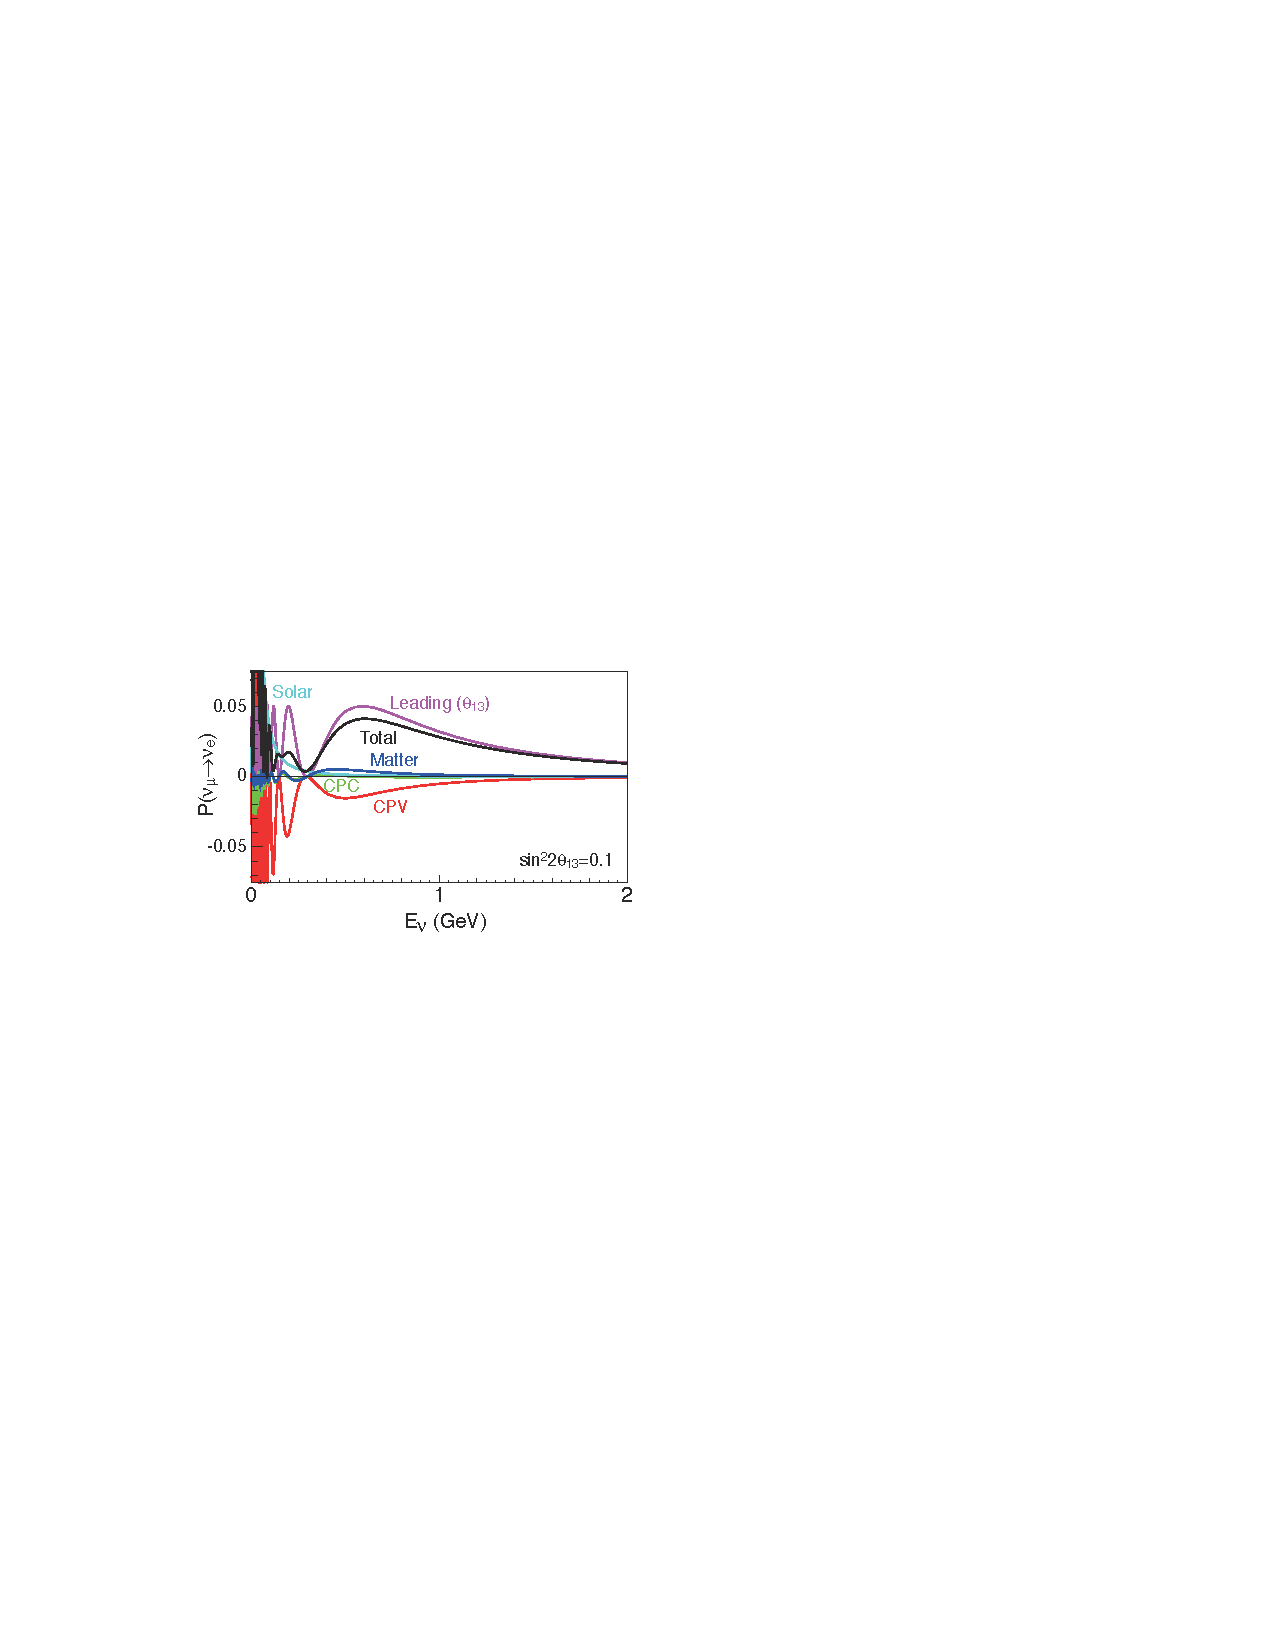
\includegraphics[width=8cm]{plotPhysics/papp_prob_2.pdf}
\caption{\label{fig:t2kappprob} Oscillation probabilities as a function of neutrino energy with L=295 km, \stot = 0.1, \dcp=$\pi/2$ and normal hierarchy. The contribution of the different terms of the oscillation probability is shown separately.}
\end{center}
\end{figure}

It is important to notice that for \nueb appearance the signs are reverted. In neutrino mode the appearance probability is maximized for normal hierarchy and $\dcp=-\pi/2$ while in anti-neutrino mode the appearance probability is maximized for inverted hierarchy and $\dcp=\pi/2$ as it is shown in Fig.~\ref{fig:t2kappnub} for the case of T2K. This figure clearly show the complementarity between \papp and \pappb and illustrates the importance of taking data also focusing anti-neutrino to fully exploit the asymmetry between \nue and \nueb apperance to measure \dcp.

\begin{figure} [h!]
\begin{center}
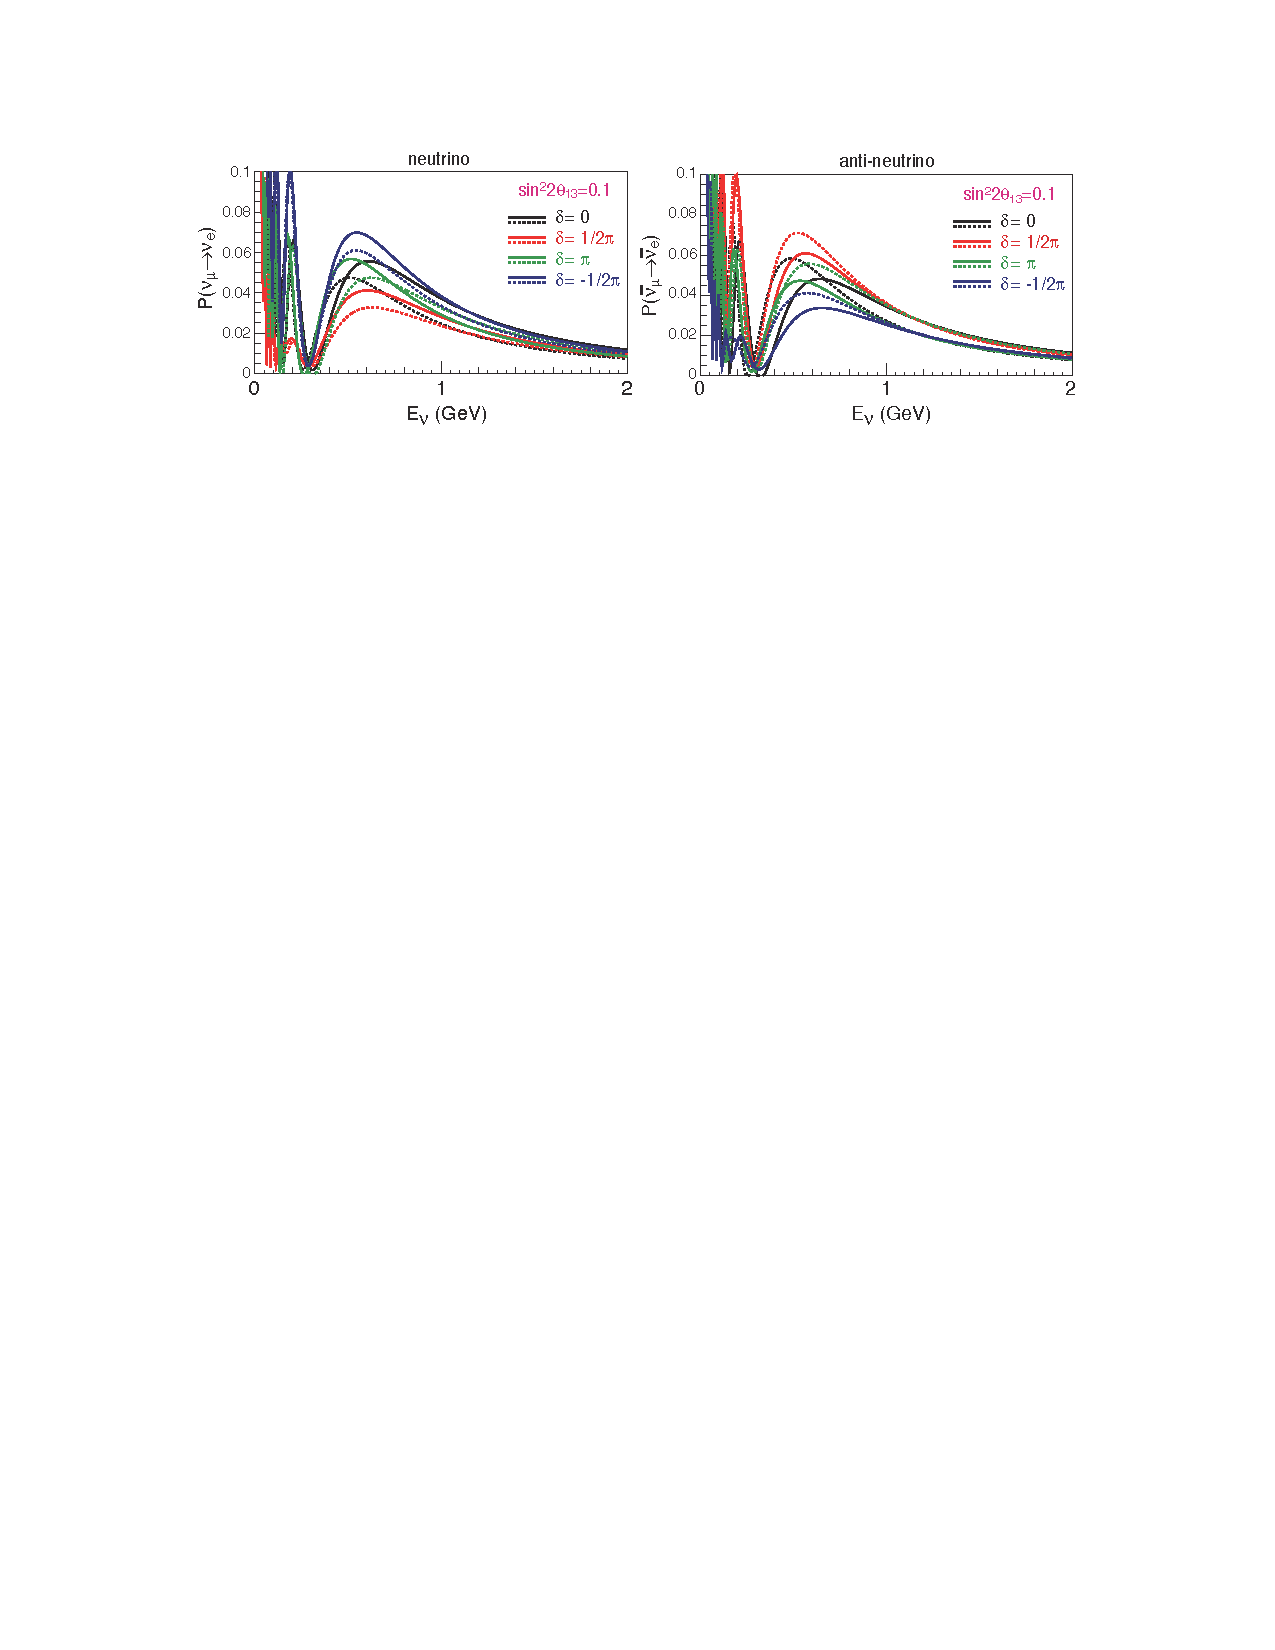
\includegraphics[width=14cm]{plotPhysics/papp_prob.pdf}
\caption{\label{fig:t2kappnub} Oscillation probabilities as a function of neutrino energy for \papp (left) and \pappb (right) with L=295 km and \stot = 0.1. The different line colors correspond to different values of \dcp while the solid (dashed) lines represent the normal (inverted) hierarchy.   }
\end{center}
\end{figure}

Finally Eq.~\ref{eq:theta13app} shows that the appearance probability also depends on the value of \thatm. Long-baseline accelerator experiments searching for \nue appearance are also sensitive to \thatm through \num disappearance.To fully take into account the correlations between oscillation parameters it is preferable to perform a joint analysis of appearance and disappearance as illustrated in~\cite{ 
 

\subsubsection{ \nue appearance in long baseline experiments}


T2K and NOVA (effect coupled to MH, NOVA if they publish)

nue appearance senstivity to delta CP (plot)


\subsubsection{ Search for \dcp in Super-Kamiokande}
SK effect in atm due to delta
\clearpage
%% global fits and summary of PMNS
\section{ PMNS model: summary}
\label{sec:summary}


The large set of experimental results on neutrino oscillations, with the exception of the anomalies that will be presented in a later section, supports the global picture of three active neutrino mixing parametrized by the PMNS mixing matrix.

Global fits have been performed on the neutrino oscillation data by two groups~\cite{nufit,fogli}.
The results of the most recent fit~\cite{nufit} are reported in Table~\ref{tab:globalfit}.


\begin{table}
\centering
\begin{tabular}{|c|c|c|}
  \hline
  Parameter & Normal Ordering & Inverted Ordering  \\ 
  \hline
$\theta_{12}$ (deg)& $33.56^{+0.77}_{-0.75}$ &  $33.56^{+0.77}_{-0.75}$\\  
  $\theta_{23}$ (deg)& $41.6^{+1.5}_{-1.2}$ &  $50.0^{+1.1}_{-1.4}$\\  
  $\theta_{13}$ (deg)& $8.46^{+0.15}_{-0.15}$ & $8.49^{+0.15}_{-0.15}$ \\  
  $\delta_{CP}$ (deg)&  $261^{+51}_{-59}$& $277^{+40}_{-46}$ \\  
  $\Delta m²_{21}$ ($10^{-5}$eV$²$)& $7.50^{+0.19}_{-0.17}$ & $7.50^{+0.19}_{-0.17}$ \\  
  $\Delta m²_{3l}$ ($10^{-3}$eV$²$)&  $2.524^{+0.039}_{-0.040}$&  -$2.514^{+0.038}_{-0.041}$\\  
  \hline
\end{tabular}
\caption{
PMNS parameters determined by a recent global fit to the world neutrino data \cite{nufit} in the hypothesis of normal ordering (second column) and inverted ordering (third column). The parameter $\Delta m²_{3l}$ is equal to $\Delta m²_{31}$ for NO and to -$\Delta m²_{32}$ for IO. }
\label{tab:globalfit}
\end{table}


At the moment, there is no significant preference for the normal or inverted ordering of the neutrino mass eigenstates. The measurement of the angles $\theta_{12}$ and 
$\theta_{13}$ and the mass squared differences $\Delta m² $ has already reached the percent precision level. This is not the case for the angle $\theta_{23}$ where the three $\sigma$ range spans the interval (38,52) degrees (see also Fig.xx) because of a mirror solution in the higher octant. Indeed, even the non-maximality of $\theta_{23}$ is not firmly established. It must be noticed that the fit reported in Table~\ref{globalfit} does not use the most recent Super-Kamiokande atmospheric results. 

The precise determination of $\theta_{23}$, of the CP-violating phase $\delta$ and of the mass ordering remains a task for future experiments.

Another long standing feature of the underlying data revealed by these fits is the 2 $\sigma$ tension between the determination of $\Delta m²_{21}$ by KamLAND on one side, and using the solar neutrino results by Super-Kamiokande, SNO and Borexino on the other side.
This tension is related to the non observation of the turn up on the lower part of the energy spectrum as predicted by the MSW effect. The observation of the day-night effect for solar neutrinos by Super-Kamiokande is also contributing to this tension. (expliquer)  


\clearpage
%% sterile neutrinos
\section{Experimental anomalies beyond the PMNS framework}
\label{sec:anomalies}

The vast majority of experimental measurement related to neutrino oscillations can be described in the framework of the PMNS matrix as reported in the previous sections. There are however some unresolved anomalies: 
\begin{itemize}
\item The LSND experiment~\cite{lsnd} reported an excess of $87.9 \pm 22.4 \pm 6.0$ events consistent with $\bar{\nu}_e p \rightarrow e^+ n$ scattering while studying $\bar{\nu}_\mu$ (endpoint energy 52 MeV) from $\mu^+$ decaying at rest, with a distance from the source to the liquid scintillator detector (167 tons) of 30~m. This might be interpreted as evidence for $\bar{\nu}_\mu \rightarrow  \bar{\nu}_e$ neutrino oscillations with $\Delta m²$ in the 0.2-10 eV$²$/c$²$ range.
\item The MiniBooNE~\cite{miniboone1,miniboone2} experiment was built to confirm the LSND claim with a muon neutrino beam at FNAL, whose peak energy is 600 MeV for neutrinos and 400 MeV for antineutrinos. It consists of a tank containing 806 tons of mineral oil equipped with 1520 PMTs at 540~m from the beam target. It reported unexplained excesses in the low-energy region of electron neutrinos and antineutrinos at the 2.8 and 3.4 $\sigma$ levels. The energy distribution of the excess in the neutrino channel is only marginally compatible within a simple two-neutrinos effective framework. 
\item The GALLEX and SAGE Gallium solar neutrino experiments have been calibrated using intense radioactive sources ($^{51}$Cr and $^{37}$Ar) placed inside the detectors~\cite{gallium}. The measured event rate is lower than expected, with the ratio of observed over expected rate deviating from 1 at the 2.8 $ \sigma$ level. This constitutes the Gallium anomaly. 
\item A recent re-evaluation~\cite{mueller} of the reactor neutrino flux combining an ab initio calculation of the spectrum related to $^{238} U$ and a revised $\beta$ inversion method for the other actinides resulted in an upward shift of the normalization by 3\% on average. A comparison of the expected with the observed antineutrino rate in short-baseline reactor experiments (L $< 100 m$ and down to 9 m for the ILL experiment and 15 m for the Bugey-4 experiment) results in a ratio of $ 0.943 \pm 0.023$~\cite{mention}. This constitutes the so-called "reactor anomaly". 
\end{itemize}

All these anomalies can be interpreted as hinting to the existence of oscillation of active neutrinos towards a sterile state with a $\Delta m²$ around 1 eV$²$/c$²$. 
It must be stressed that, while all the measurements related to the various sectors of the PMNS matrix have been confirmed by several experiments with very different techniques (for instance the $ \theta_{23}$ oscillations have been observed by experiments using atmospheric neutrinos and by long baseline experiments), each of this anomaly is rather isolated. Moreover, the statistical significance is far from being compelling and does not exceed 3 $\sigma$. 
Repeated and numerous attempts have been made to interpret these anomalies in models where the three known active neutrinos mix with a fourth sterile state (3+1) or with two new sterile states (3+2).
 In the 3+1 model, in the limit where the phases relative to $\Delta m^2_{21}$ and $\Delta m^2_{31}$ can be neglected  the survival probability reads
\begin{equation}
P(\nu_e \rightarrow \nu_e) = 1 - 4 |U_{e4}|^2 (1 - 4 |U_{e4}|^2) \sin^2 \frac{\Delta m^2_{41}L}{4E} = 1 - \sin^2 \theta_{ee} \sin^2 \frac{\Delta m^2_{41}L}{4E}
\end{equation}
where the effective mixing angle $\theta_{ee}$ is defined as $\sin^2 \theta_{ee} = 4 |U_{e4}|^2 (1 - 4 |U_{e4}|^2)$. 

To interpret the results of the LSND and MiniBooNE experiments both the $U_{e4}$ and the $U_{\mu 4}$ matrix elements should be different from zero and the appearance probability reads
\begin{equation}
P(\nu_\mu \rightarrow \nu_e) = |U_{e4} U_{\mu 4}|^2  \sin^2 \frac{\Delta m^2_{41}L}{4E} = \sin^2 2 \theta_{\mu e} \sin^2 \frac{\Delta m^2_{41}L}{4E}
\end{equation}
with $\sin^2 \theta_{\mu e} = 4 |U_{e4} U_{\mu 4}|^2$.
The formulae are more complex in 3+2 models, where the number of free parameters of the models is larger.

Global fits to the world dataset corresponding to these anomalies and all other experimental results on neutrino oscillations measurements and searches have been attempted \cite{giuntirev,kopp}. The result is that there is a strong tension between appearance experiments like LSND and MiniBooNE and the negative results from disappearance experiments like CDHS. Oscillations in the $\bar{\nu}_\mu \rightarrow  \bar{\nu}_e$ channels inevitably entail disappearance in the 
$\bar{\nu}_\mu \rightarrow  \bar{\nu}_\mu$ channel with the same L/E range. This disappearance has not been observed. The compatibility of appearance and disappearance data is at the level of $10^{-4}$. More complex models like 3+2 do not alleviate this tension. 

\begin{figure}[htbp]
\begin{minipage}[c]{.46\linewidth}
%\begin{minipage}[c]
   	      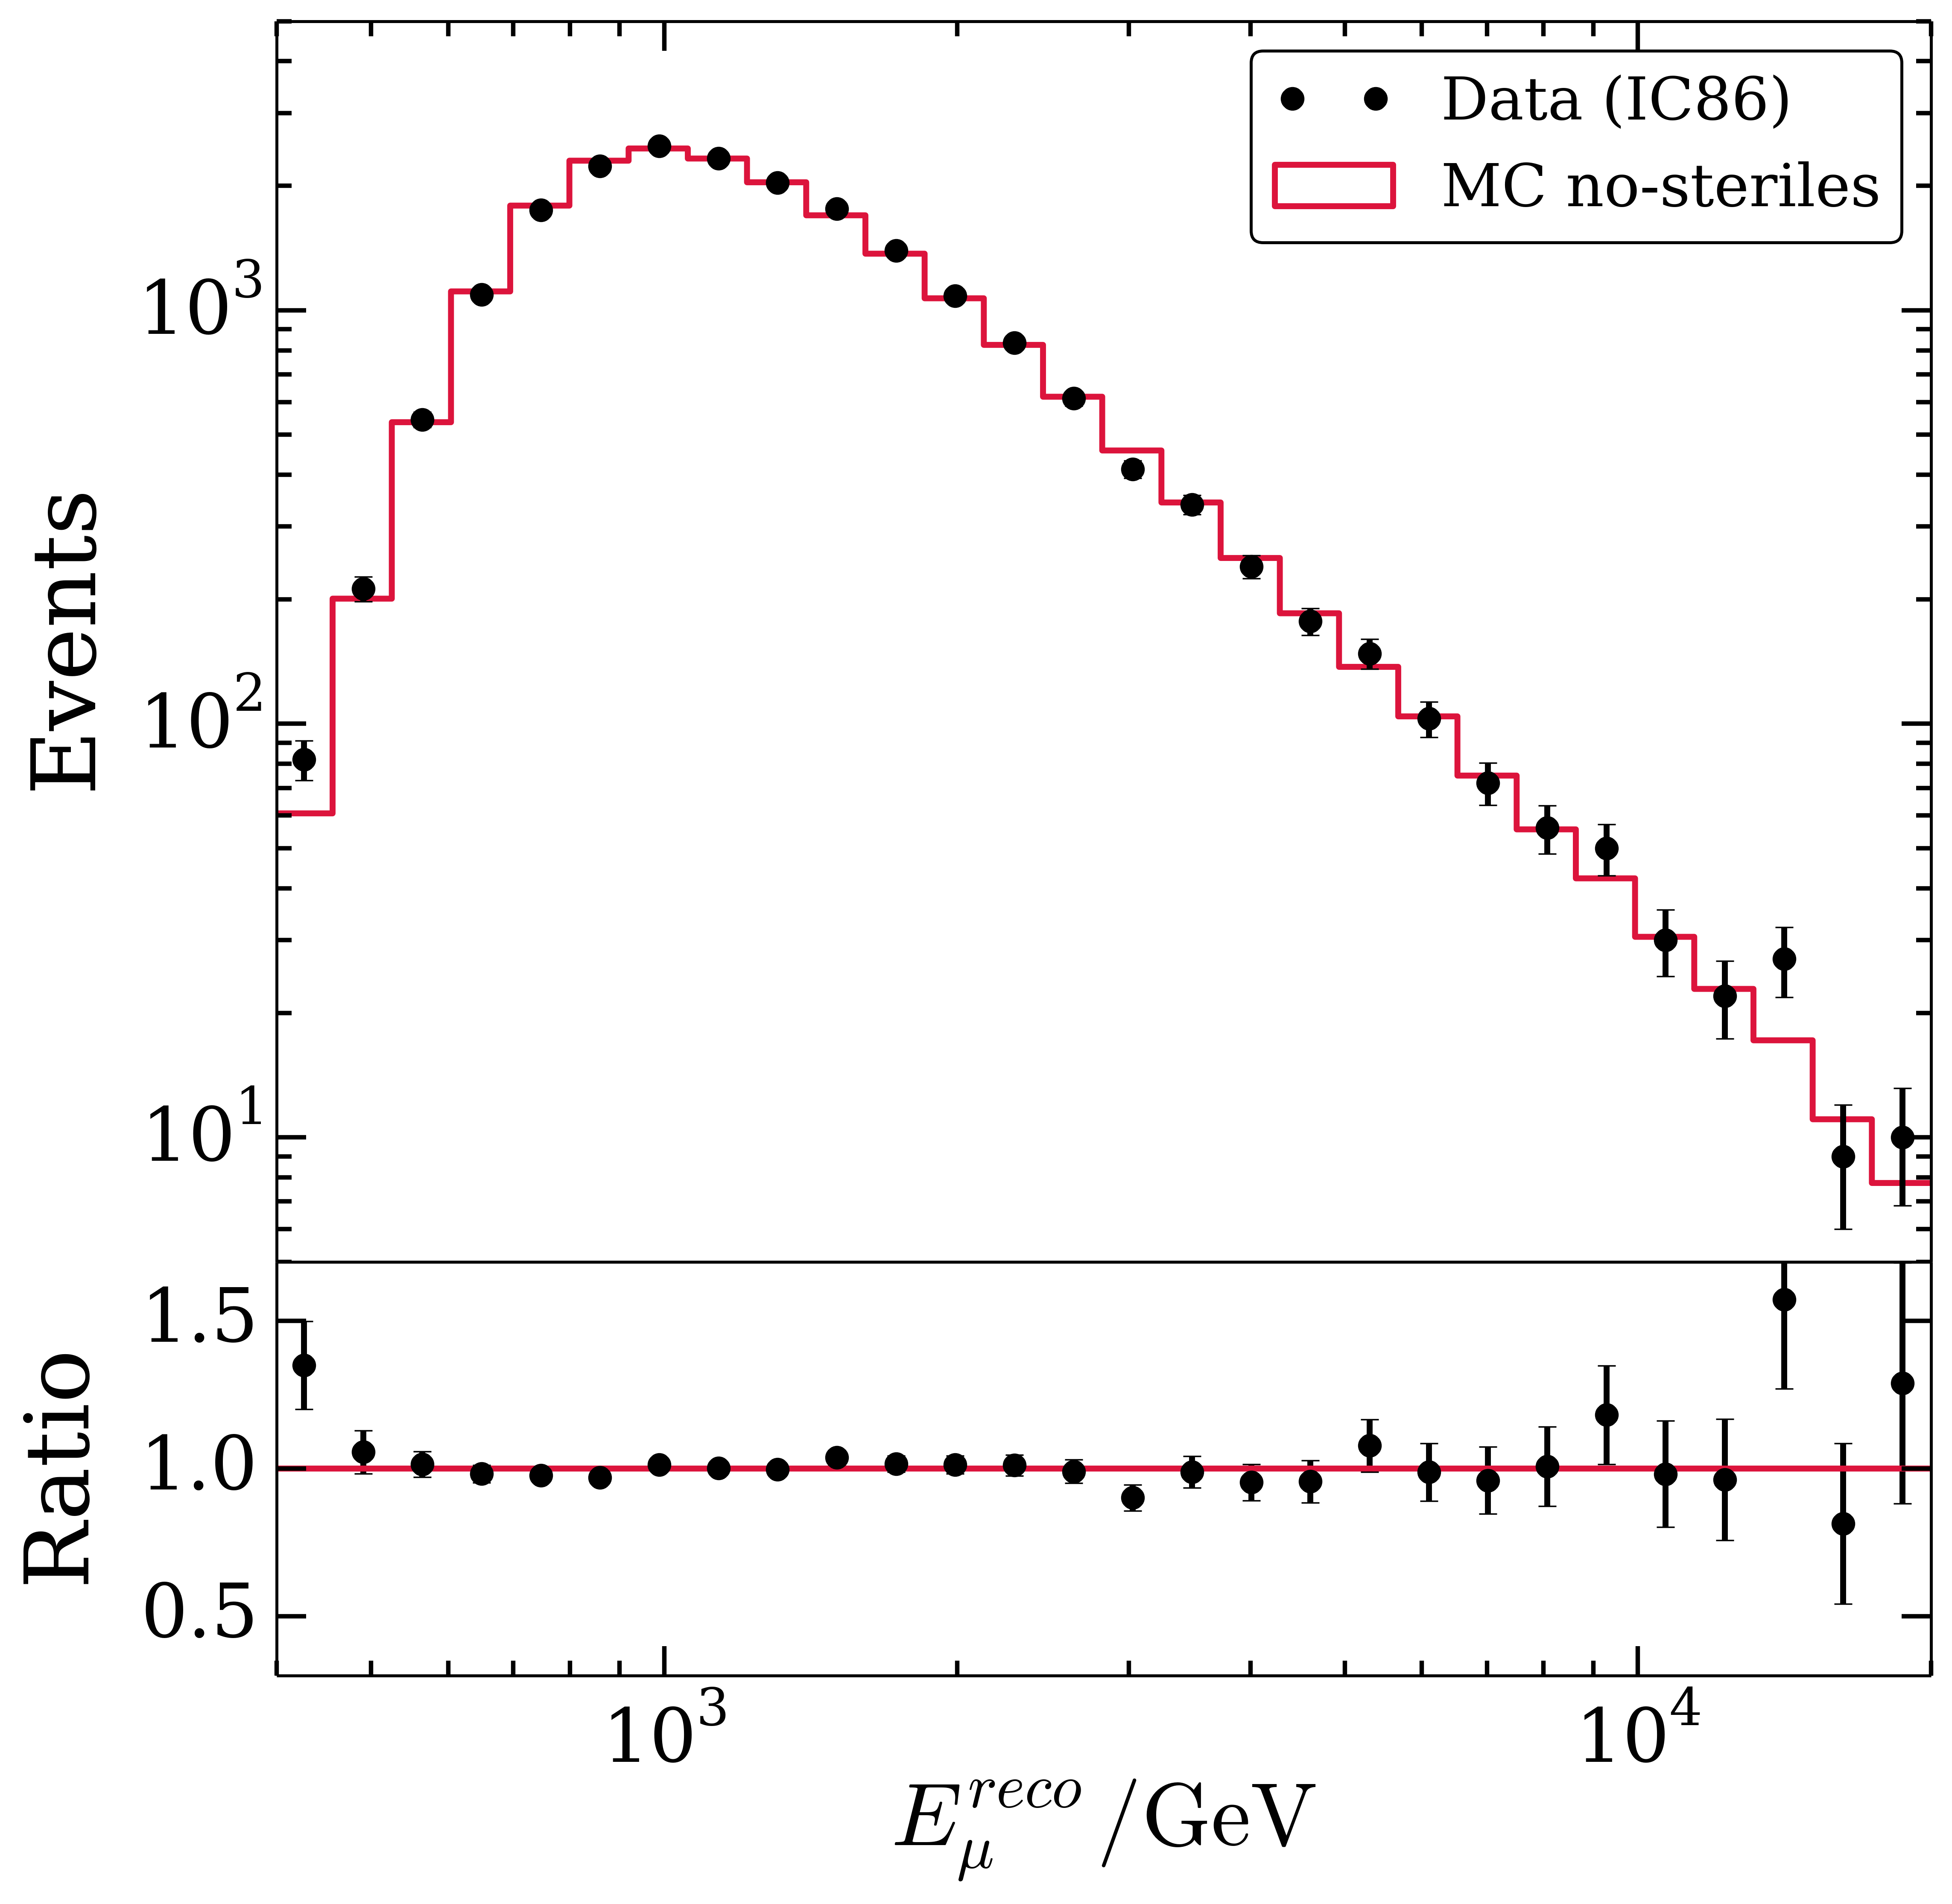
\includegraphics[width=0.9\linewidth]{figures/EnergyDist-2.png}
   \end{minipage} \hfill
   \begin{minipage}{.46\linewidth}
      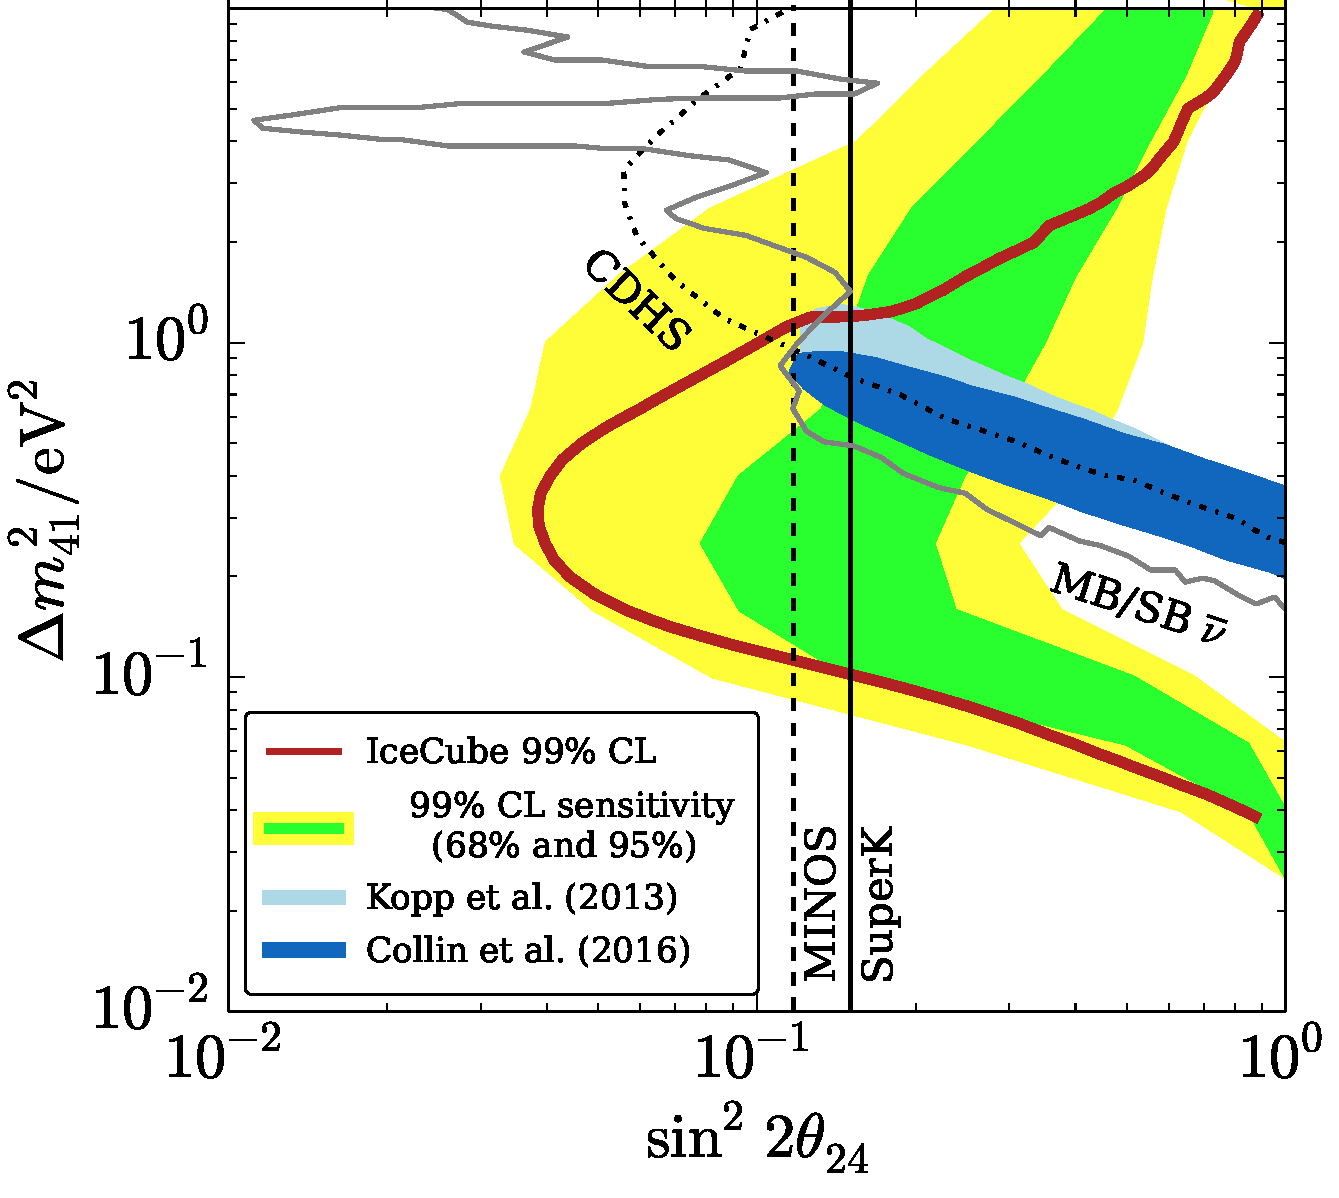
\includegraphics[width=0.9\linewidth]{figures/icecube-sterile-crop.pdf}
   \end{minipage}
    \caption{The reconstructed energy distribution of atmospheric $\nu_\mu$ events observed by the IceCube experiment compared to the prediction without sterile neutrinos (left). 
The 99%
(red solid line) CL contour in the $\Delta m^2_{41}$ versus $\sin² (2 \theta_{24}$ obtained by the IceCube experiment is shown with bands containing
68\% (green) and 95\% (yellow) of the 99\% contours in sim-
ulated pseudo-experiments, respectively. The contours and
bands are overlaid on 90\% CL exclusions from previous experiments [7–10], and the MiniBooNE / LSND 90\% CL allowed
region from [12, 13, 21] assuming $|U_{e4}|^2 = 0.023$.  }
 \label{fig:icecube-sterile}
\end{figure}

Very recent data confirm this picture and actually bring more experimental evidence against the LSND and MiniBooNE anomalies.
The IceCube has studies the atmospheric muon neutrino spectrum in the range 320 GeV to 20 TeV~\cite{icecubeste}. Muon neutrino mixing with a sterile state with $\Delta m²_{41}$ in the 1 eV$^2$ range would strongly deplete the observed antineutrino spectrum for 3+1 models mainly due to MSW resonance effects during neutrino propagation in the Earth. The deficit can reach 11\% for the bin with the largest effect in the distribution of reconstructed energy and zenith angle. Similar effects would deplete the neutrino spectrum for 1+3 models. No depletion is observed in a sample of 20145 well reconstructed muons registered with an 86 strings configuration in 2011 and 2012. They set strong limits in the 
$\Delta m^2_{41}$ versus $\sin² (2 \theta_{24}$ plane. The allowed region from the appearance experiments LSND and MiniBooNE is excluded at the 99\% CL (Fig.~\ref{fig:icecube-sterile}).  

An interesting limit has been set by a combined analysis of the MINOS, Daya Bay and Bugey-3 data. MINOS is sensitive to a sterile neutrino as active (mainly $\nu_\mu$ in this case)-sterile mixing would modify the shape and normalization of charged current and neutral current events in the near and far detectors.
It can therefore set limits on $|U_{\mu 4}|$. Bugey-3 and Daya Bay data can be used to constrain electron antineutrino disappearance and place limits on $|U_{e 4}|$. The combination of these three experiments excludes the phase space allowed by the LSND and MiniBooNE experiments below 0.8 eV$^2$ at 95 \% CL~\cite{dayabaycomb}. 

The reactor and Gallium anomalies are not in such a conflict with other measurements. In this sector, recent developments have focussed on the reliability of systematic uncertainty related to the understanding of the reactor antineutrino flux. The observation of the 5 MeV bump has indeed brought under close scrutiny the method to compute the reactor antineutrino flux. The conclusions of recent studies \cite{hayes,vogel} are that several uncertainties might have been underestimated. For instance, 30\% of the flux comes from forbidden transitions. The effect of various shape corrections applied to forbidden transitions has been investigated and it leads to a 4-5\% uncertainty on the reactor antineutrino flux. Taking into account this uncertainty would considerably release the tension at the origin of the reactor anomaly.

A new generation of reactor neutrino experiments (STEREO, SOLID, NEUTRINO-4, DANSS, see \cite{othervsbl} for a review) has been built to investigate in detail the possible mixing of $\nu_e$ with a sterile state with $\Delta m²_{41}$ in the 1 eV$^2$ range.
Indeed this mixing would induce a deformation of the spectrum if the detector is placed close enough (L$\simeq$ 10m) to the reactor core. These experiments will take data starting in 2017 or earlier and so new results on this hot topic are expected soon.
The SOX experiment \cite{cribier} will deploy an intense $^{144}$Ce antineutrino source very close to the Borexino detector with data taking in 2018.

The three Liquid Argon detector set-up SBN \cite{sbnfnal} is in construction at FNAL The MicroBooNE (170 t, L=470m) Liquid Argon detector has been built on the Booster Neutrino beam, the same beam used by MiniBooNE. It will be completed by the refurbished ICARUS detector (760 t) placed at 600~m and by the LAr1-ND near detector (220 t)  at 110~m from the production target, for the investigation of these anomalies both in the appearance and in the disappearance channels. This set of detectors will be able to probe the LSND appearance excess with a sensitivity of 5 $\sigma$. The installation will be completed in 2018.    


\clearpage
%% future experiments
\section{Perspectives for future experiments 20pg MZ}
\label{sec:future}


\subsection{Existing projects: T2K NOVA}

T2K statx10 + antinu data no MH

NOVA MH sensitivity (depends on delta)

(where do we add  SK ?)

increased sensitivity to theta23


\subsection{middle term}

JUNO prec measurement of theta12 and Dm21

method NH/IH, critics Parke

depends on E exp resolution, not demonstrated

PINGU/ORCA discussion sensitivity MH (numu->numu vs showers)

INO distinguishes btw numu and numubar status ? 


\subsection{Long term: HyperKamiokande, DUNE}

DUNE new technology LAr 40 kt new beam

decouples CP violation from MH with nu/nubar beam

HyperK 500 kt fiducial (finance ?) upgraded T2K beam

complementarity DUNE/HK

\section{Conclusions}
\label{sec:conc}

The field of neutrino oscillations has recently shown a rapid progress and is now entering the precision period. Indeed, after the establishment of neutrino oscillations as the mechanism behind the anomalies observed in the study of solar and atmospheric neutrinos, the measurement of the last mixing angle \thint, several confirmations and more accurate measurements have established the PMNS three active neutrino paradigm as the framework capable of interpreting a vast array of experimental results. 

A few anomalies, most notably the LSND anomaly, can not be interpreted in the PMNS framework. Recent experimental results have not confirmed these anomalies, that have been the object of an intense scrutiny and debate. An experimental program is underway that will provide new more sensitive tests of these anomalies, with reactor neutrinos, a radioactive source and with short baseline accelerator based experiments. These experiments will provide their results in the next few years, before 2020. Therefore in a few years we should be able to either remove these anomalies from the list of open questions, or on the contrary face a major exciting discovery.  

For most of the parameters of the PMNS matrix and for the squared mass differences the measurements have attained the \% precision and certainly great attention needs to be devoted to the experimental systematic uncertainty to make further progress. A robust and precise control of the neutrino flux is needed for future experiments devoted to the improvement of the experimental accuracy. This calls for a full fledged program of auxiliary experiments and measurements, for instance in the field of hadro-production experiments like NA61/SHINE. It calls also for a renewed program to establish a reliable model for the neutrino nucleus cross-section, where new phenomenological investigations and new high precision data will be major ingredients. The goal is to reach a control at the \% level, as opposed to 10\% or worse uncertainty level of the current uncertainties.

A rich experimental program is today under preparation to answer the remaining open questions, like the precise measurement of the $\theta_{23}$ mixing angle, its deviation from the maximal value $\pi/4$ and its octant, the question of the mass ordering and the determination of the CP violating phase \dcp. These are fundamental questions and measurements in this field are likely to dominate the scene of experimental particle physics in the next years. Partial answers to these questions will come from the running long baseline experiments T2K and \nova.
The question of mass ordering will be addressed to a certain extent by non-accelerator program using either atmospheric neutrinos or nuclear reactors. 
In the next decade two major projects, DUNE and Hyper-Kamiokande, are in preparation to provide high precision measurements. 









\section*{Acknowledgements}

We thank Davide Franco, Marco Martini, and Boris Popov for reading the manuscript and providing useful comments.

%% The Appendices part is started with the command \appendix;
%% appendix sections are then done as normal sections
%% \appendix

%% \section{}
%% \label{}

%% If you have bibdatabase file and want bibtex to generate the
%% bibitems, please use
%%
%\begin{thebibliography}

%\bibliography{biblio}

%\end{thebibliography}


%% else use the following coding to input the bibitems directly in the
%% TeX file.

%\bibliographystyle{unsrt}
\bibliography{biblio}% Produces the bibliography via BibTeX.                                                                          

%\addcontentsline{toc}{chapter}{\numberline{}Bibliography}%\bibliography{t2kpub}
%\bibliography{biblio.bib}

%% \bibitem[Author(year)]{label}
%% Text of bibliographic item

%\bibitem{ref:Ga2002}
%T. Gaisser and M. Honda, Flux of Atmospheric Neutrinos, Ann. Rev. Nucl. Part. Sci. 52 (2002) 153.
%
%\bibitem{ref:midori}
%M. Honda, T. Kajita, K. Kasahara, S. Midorikawa  Phys. Rev. D 83 (2011) 123001. 
%
%\bibitem{ref:barr}
%G. Barr, et al. Phys. Rev. D 70 (2004) 023006.
%
%\bibitem{ref:fluka}
%G. Battistoni et al. Astropart. Phys. 19 (2003) 269.
%%\bibitem{ref:}
%
%\bibitem{ref:achar}
%C. Achar, et al. Phys. Lett. 18 (1965) 196.
%
%\bibitem{ref:reinesAtm}
%F. Reines, et al. Phys. Rev. Lett. 15 (1965) 429.
%
%\bibitem{ref:skatm98}
%Y. Fukuda, et al. (Super-Kamiokande Collab.) Phys. Rev. Lett. 81 (1998) 1562.
%
%\bibitem{ref:sk-atm-2006}
%J. Hosaka et al., (Super-Kamiokande Collab.) Phys. Rev. D 74, 032002 (2006),
%
%
%\bibitem{ref:icecubedis}
%%M. Aartsen, et al. (IceCube Collab.) Phys. Rev. Lett. 111 (2013) 081801.
%M.G. Aartsen et al., Nuclear Physics B 908  161 (2016).
%
%\bibitem{ref:kopp}
%S. Kopp, Phys. Rep. 439 (2007) 101
%
%\bibitem{ref:beavis}
%D. Beavis et al. 
%%“P889: Long Baseline Neutrino Oscillation Experiment at the AGS,”
%Report No. BNL-52459, 1995.
%
%\bibitem{ref:k2k}
%M. H. Ahn et al, (K2K Collab.), Phys. Rev. D 74 (2006) 072003. 
%
%\bibitem{ref:skatauapp}
%Abe K, et al. (Super-Kamiokande Collab.) Phys. Rev. Lett. 110 (2013) 181802.
%
%\bibitem{ref:opera}
%N. Agafonova et al. (OPERA Collaboration)
%Phys. Rev. Lett. 115 (2015) 121802.
%
%\bibitem{ref:opera2}
%A. Di Crescenzo, Nuclear and Particle Physics Proceedings 265–266 (2015) 186–188.
%
\end{document}

%\endinput
%%
%% End of file `elsarticle-template-harv.tex'.
